\begin{frame}
    \frametitle{Положения, выносимые на защиту}
    \begin{itemize}
  		\item Модификация метода Вилена по выявлению звезд-кандидатов в $\Delta\mu$-двойные;
  		\item Адаптация шейплет-формализма для детектирования скрытых двойных звездных изображений;
  		\item Выявление 259 звезд--кандидатов в маломассивные двойные системы;
  		\item Подтверждение двойственности пяти систем методами высокого разрешения.
    \end{itemize}
\end{frame}

\begin{frame}
\frametitle{Ближайшее население}
\begin{figure}[pt]
  \centering
   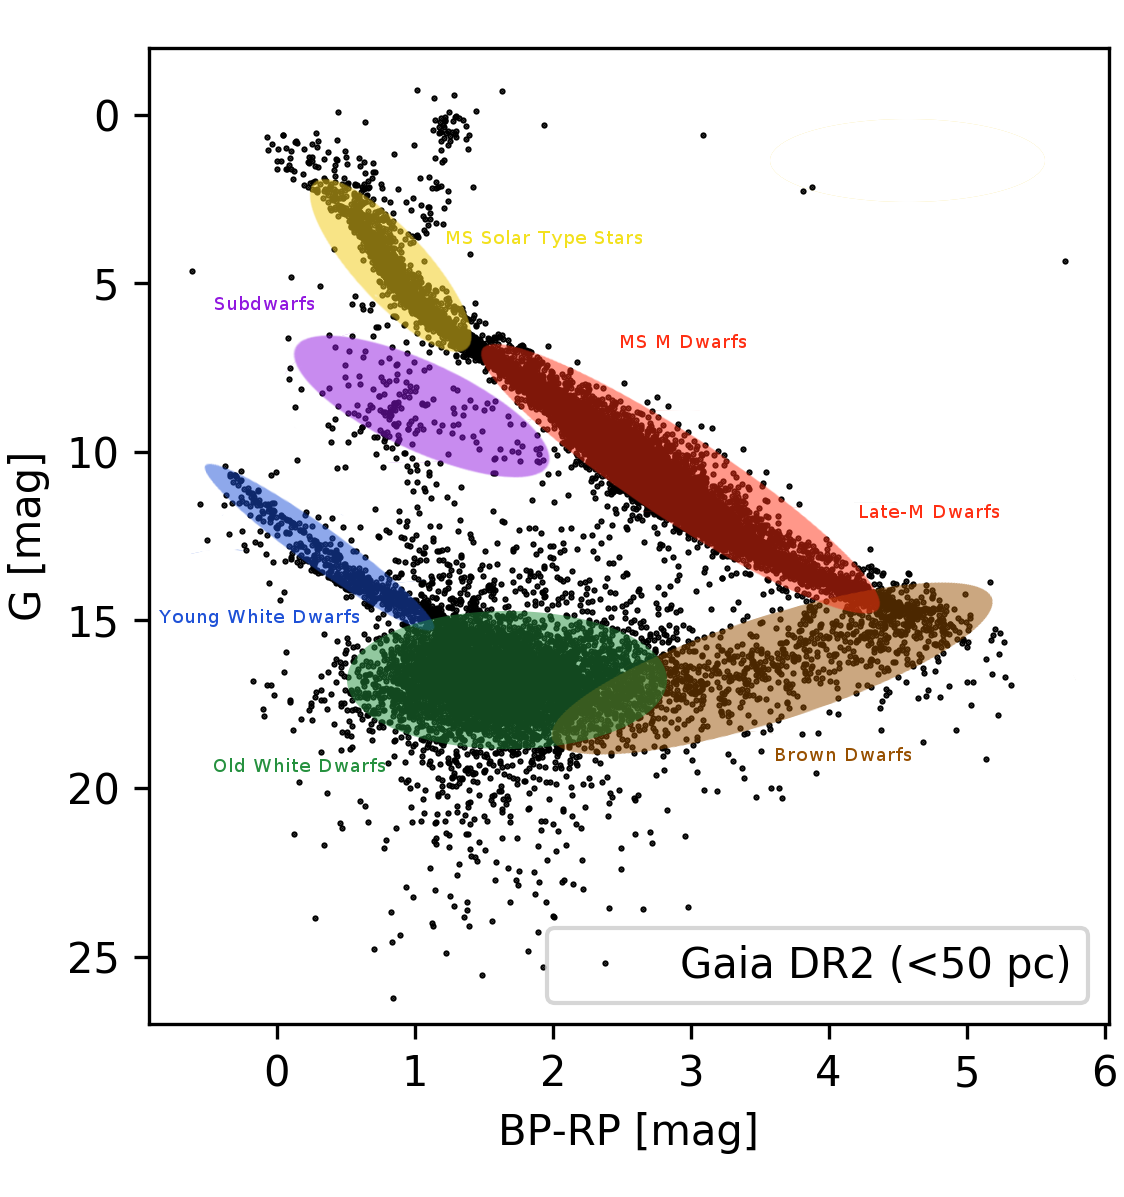
\includegraphics[width=0.7\linewidth]{gaia50types}
\end{figure}
\end{frame}

\begin{frame}
\frametitle{Задачи карликов}
\begin{itemize}
  \item Наблюдения и сбор статистических данных
  \item Уточнение зависимостей <<масса -- радиус>> и <<масса -- светимость>>
  \item Построение и тестирование физических моделей маломассивных звезд
\end{itemize}
\end{frame}

\begin{frame}
\frametitle{Изохроны}
\begin{columns}
 \column{0.6\textwidth}
	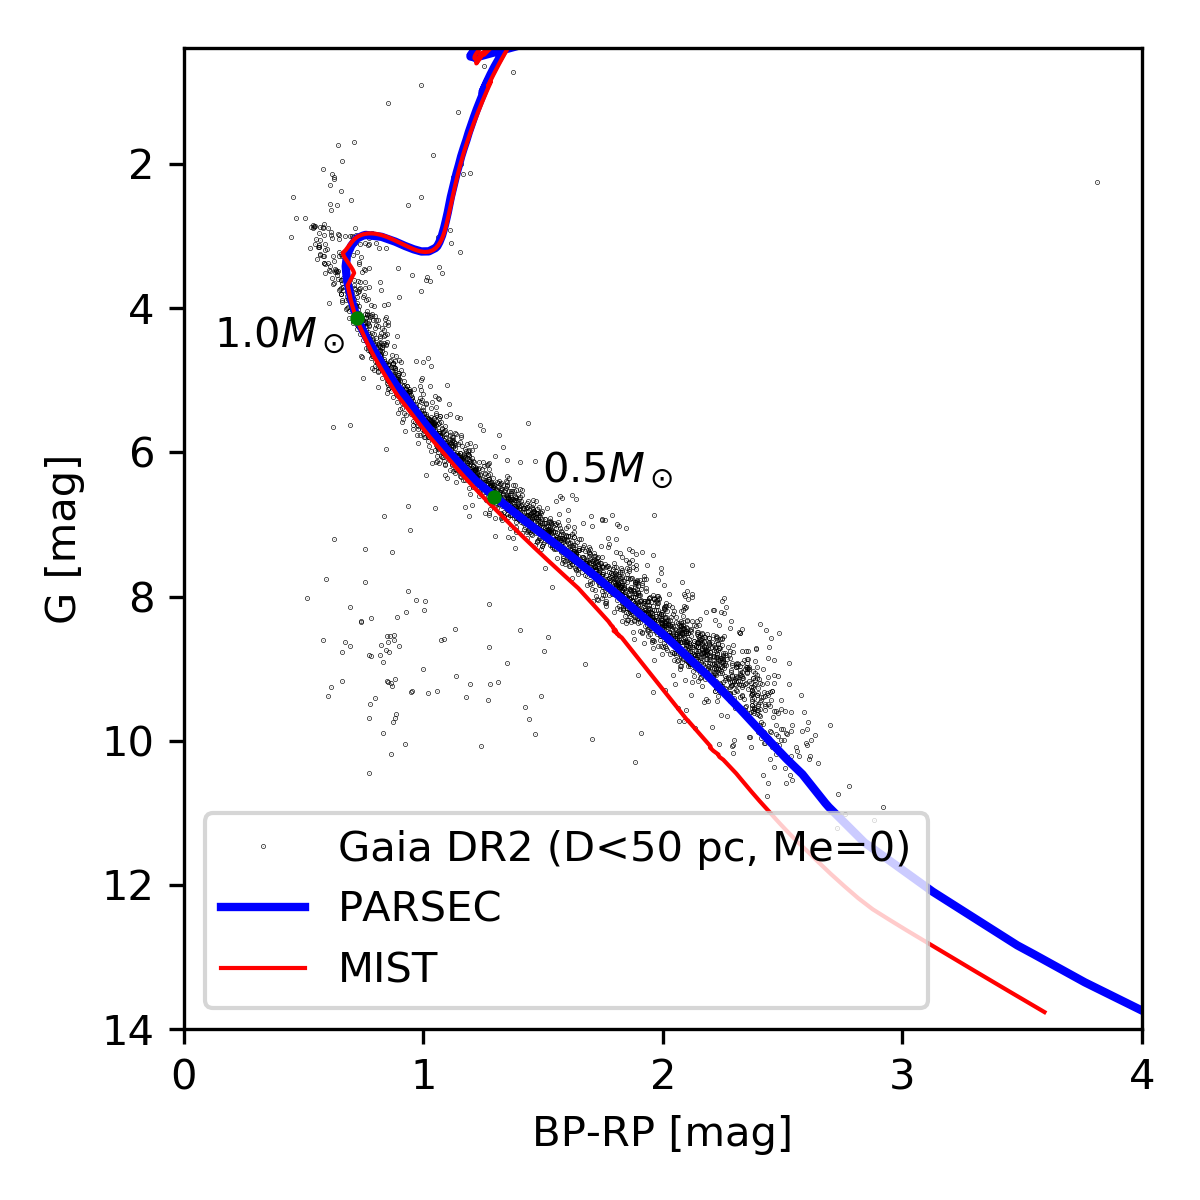
\includegraphics[width=0.99\linewidth]{parsec-mist-gaia}
 \column{0.4\textwidth}
 {\scriptsize PARSEC (Bressan et al., 2012)} \\
 {\scriptsize MIST (Choi et al., 2016)} \\
 {\scriptsize $[M/H]=0$} \\
 {\scriptsize возраст --- 5 Gy} \\
 {\scriptsize G --- mag для фильтра Gaia} \\
\end{columns}
\end{frame}

\begin{frame}
\frametitle{Эмпирический подход}
\begin{figure}[pt]
  \centering
  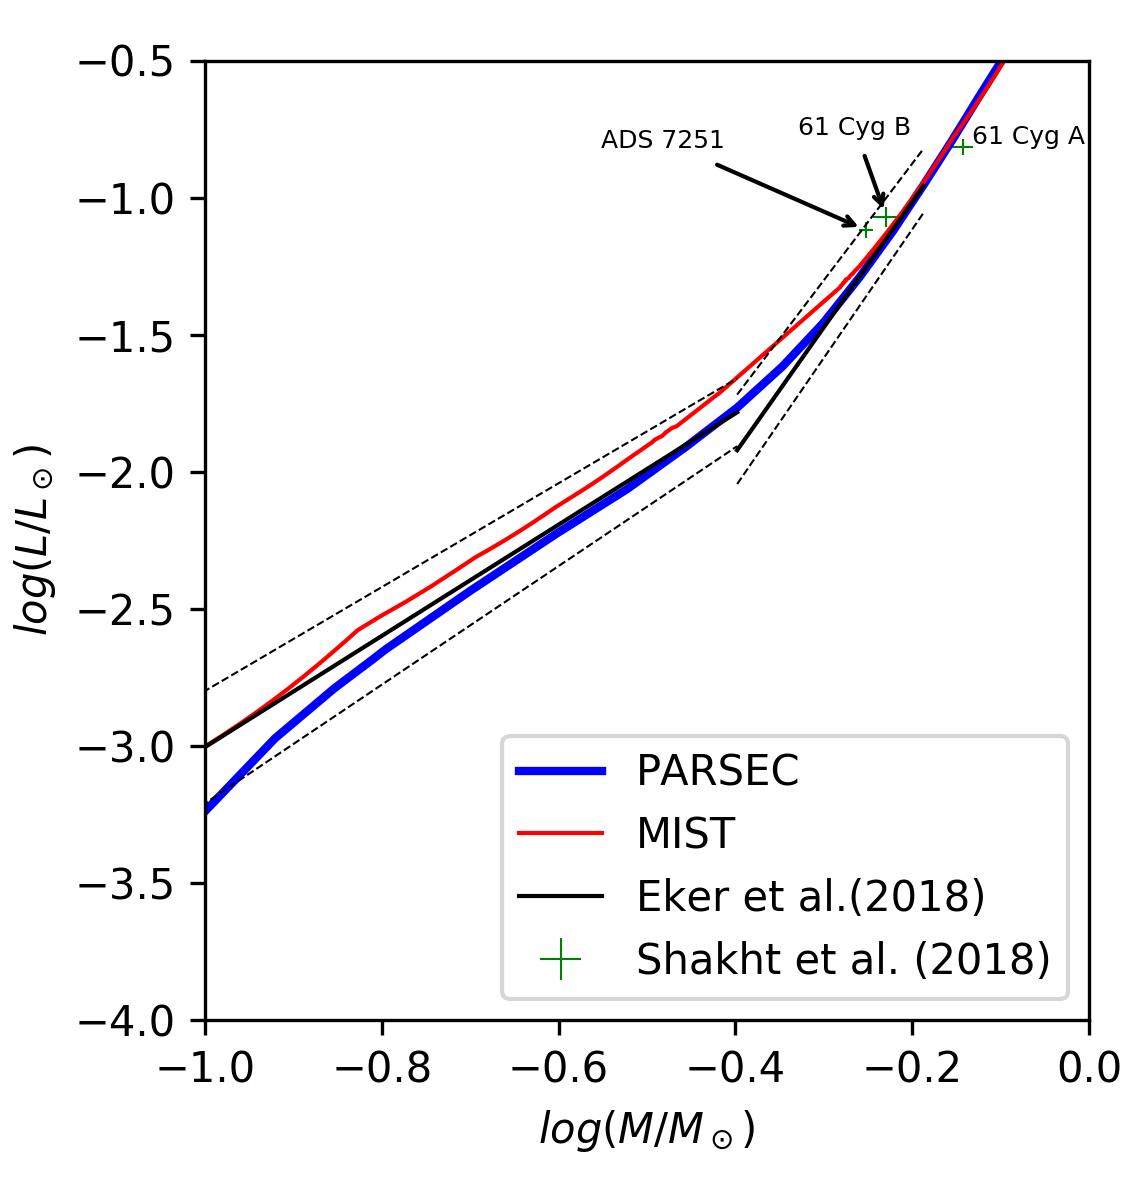
\includegraphics[width=0.7\linewidth]{mass-lum}
\end{figure}
\end{frame}

\begin{frame}
\frametitle{Коричневые карлики и Gaia}
\begin{itemize}
  \item до 90\,\% энергии корчневых карликов излучается в ИК диапазоне (Chabrier et al., 2005)
  \item диапазон наблюдений Gaia: $\lambda <1.05$~ мкм (The Gaia mission, 2016)
\end{itemize}

В окружности 20 пк Gaia может полностью исследовать звезды до L5 (Kirkpatrick et al., 2019).
\end{frame}

\begin{frame}%{{\tiny \it Зачем нужны маломассивные компоненты двойных систем?}}
\frametitle{Проблемы карликов}
\begin{itemize}
\item Имеет место дефицит надежно определенных масс для звезд с $M<0.7 M_{\odot}$.
\item Калибровка моделей привязана к тесным системам, где оценки M и L могут быть искажены систематическими ошибками (несферичность, взаимный нагрев).
%\item Крайне важно получить независимые оценки масс маломассивных звезд.
\end{itemize}
\end{frame}

\begin{frame}%{{\tiny \it Физические модели процесса звездообразования}}
\frametitle{Физическая модель звездообразования}
\begin{columns}
\column{0.6\textwidth}
	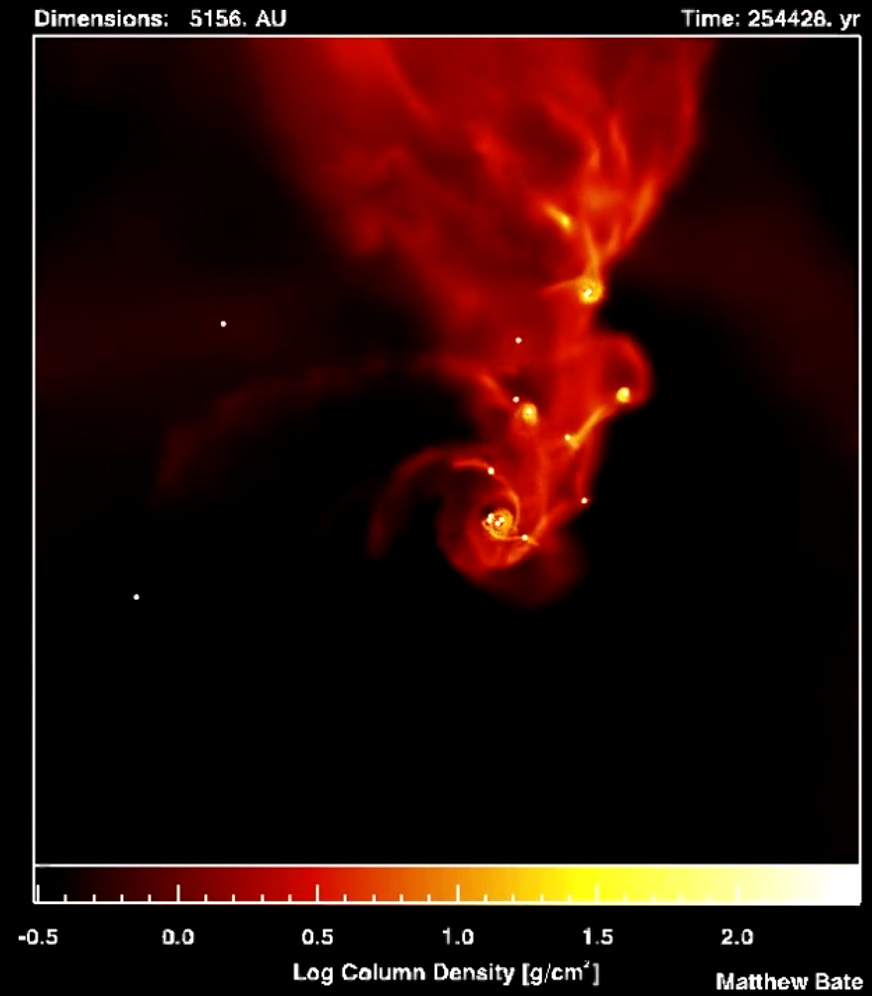
\includegraphics[width=0.99\columnwidth]{Bate-preview}
\column{0.4\textwidth}

 {\footnotesize Bate, 2019: \\
 \begin{itemize}
    \item химический состав
    \item влияние космических лучей
    \item нагрев газа и пыли из-за излучения звезд
    \item процессы диффузии и переноса излучения
    \item $M_{cloud}=500M_{\odot}$
    \item $\Sigma M_{stars} \approx 100M_\odot$
    \item $Median~M_{star} \approx 0.15M_\odot$
 \end{itemize}
 }
\end{columns}
\end{frame}

\begin{frame}%{{\tiny \it Физические модели процесса звездообразования}}
\frametitle{Физическая модель звездообразования}
\begin{center}
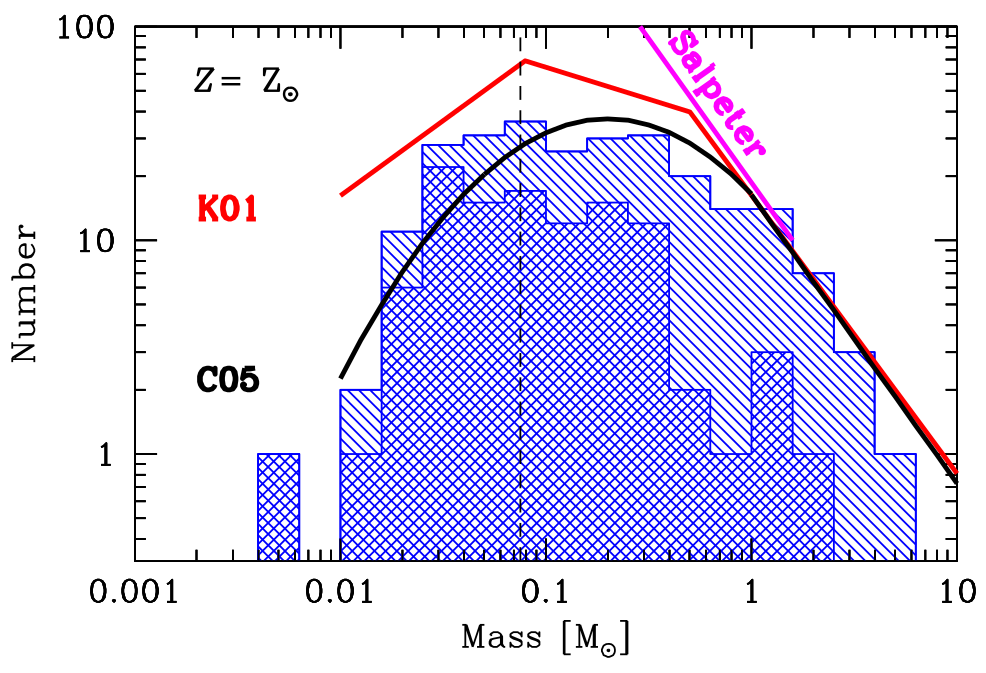
\includegraphics[width=0.8\textwidth]{Bate-IMF}
\end{center}
{\scriptsize Заштрихована область --- звезды, для которых темп аккреции менее $10^{-7}M_\odot/yr$. (Bate, 2019)}
\end{frame}

\begin{frame}%{{\tiny \it Физические модели процесса звездообразования}}
\frametitle{Физическая модель звездообразования}
\begin{center}
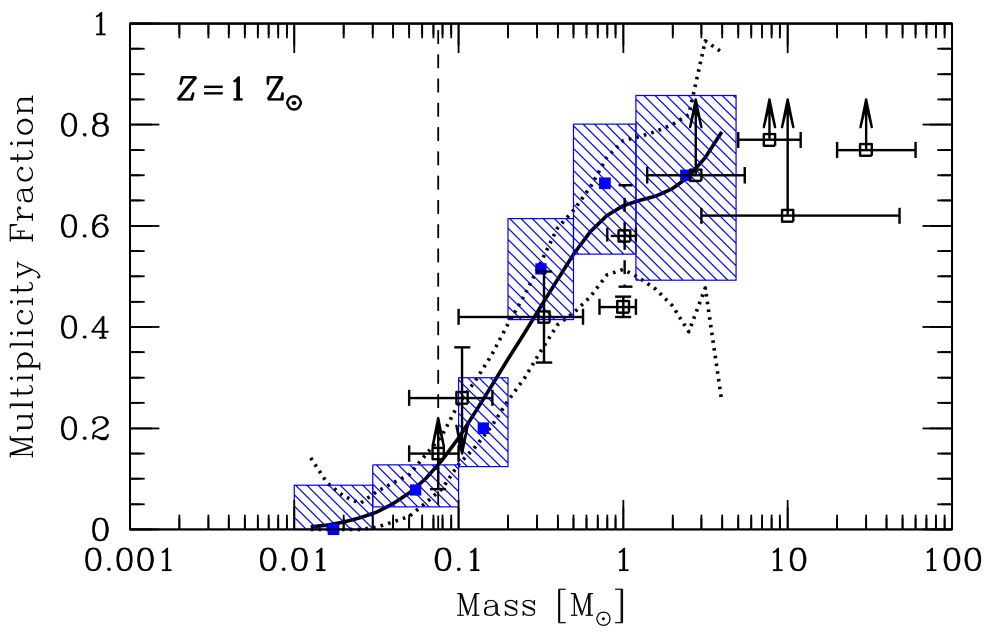
\includegraphics[width=0.8\textwidth]{Bate-BF}
\end{center}
{\scriptsize Стороны прямоугольников = $1\sigma$, кривая~---~аппроксимация, квадраты~---~наблюдения. (Bate, 2019)}
\end{frame}

\begin{frame}%{{\tiny \it Физические модели процесса звездообразования}}
\frametitle{Физическая модель звездообразования}
\begin{columns}
\column{0.6\textwidth}
	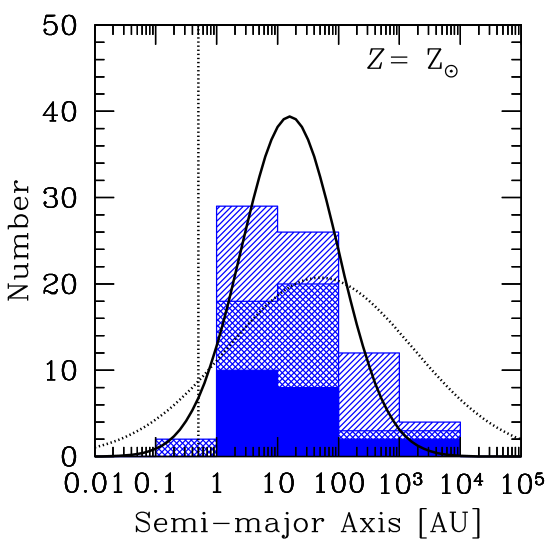
\includegraphics[width=0.99\columnwidth]{Bate-a-distr}
\column{0.4\textwidth}
 {\scriptsize Гистограммы для двойных, тройных и более звезд.} \\
 {\scriptsize Сплошная: Janson et al.(2012)} \\
 {\scriptsize Пунктир: Raghavan et al. (2010)} \\
 {\scriptsize (Bate, 2019)}% \\
% {\scriptsize Гистограммы для двойных, тройных и более звезд. Сплошная кривая: Janson et al.(2012), пунктир - Raghavan et al. (2010). (Bate, 2019)}
\end{columns}
\end{frame}

\begin{frame}
\frametitle{Эволюция доли двойных}
\begin{columns}
\column{0.7\textwidth}
	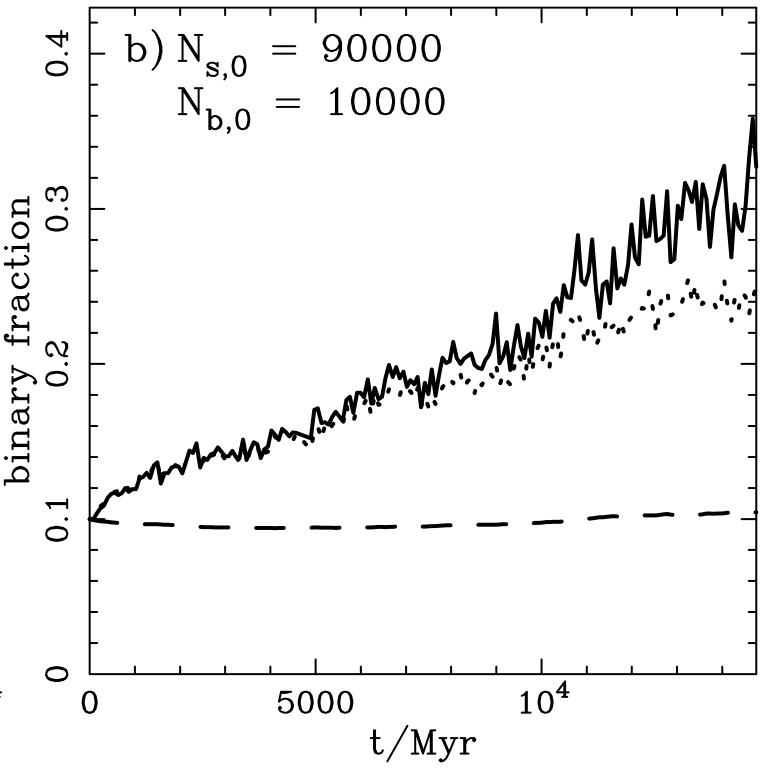
\includegraphics[width=0.99\columnwidth]{Hurley}
\column{0.3\textwidth}
 {\footnotesize Hurley et al., 2017}%:\\ 100\,000~звезд}% \\
\end{columns}
\end{frame}


\begin{frame}
\frametitle{Тесные системы в Gaia}
\begin{center}
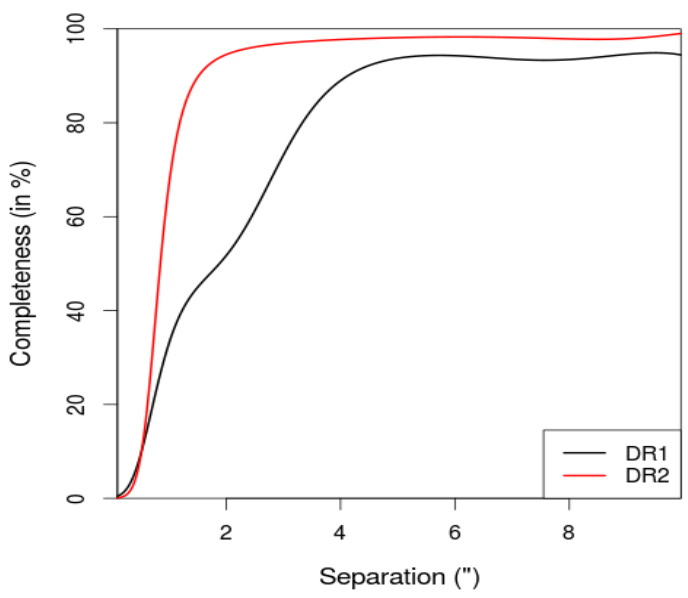
\includegraphics[width=0.6\textwidth]{gaia-complitness-for-binaries}
\end{center}
{\footnotesize Угловое разрешение Gaia~DR2 $\approx 2~arcsec$. Arenou et al., 2018.}
\end{frame}

\begin{frame}
\frametitle{Тесные системы в Gaia}
\begin{columns}
\column{0.6\textwidth}
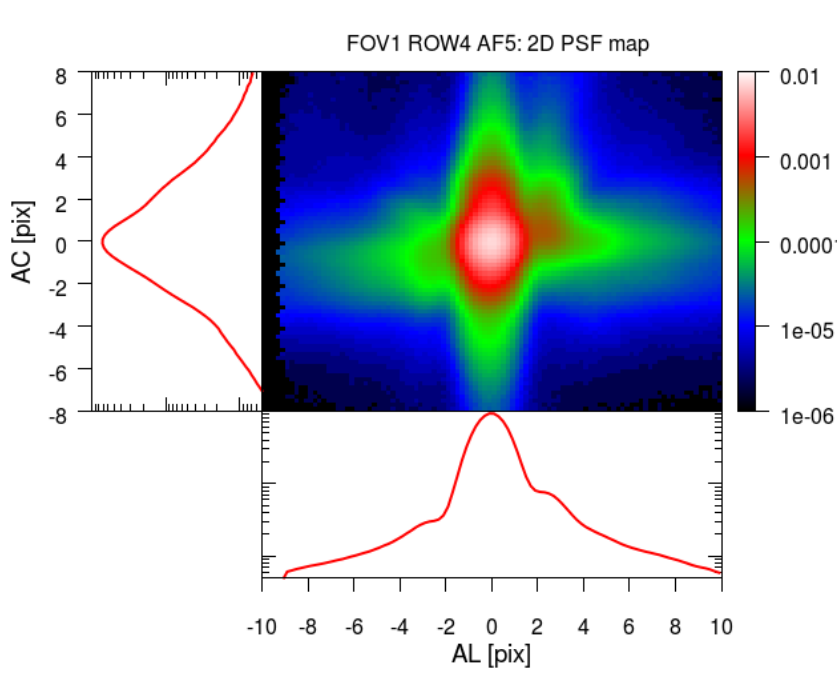
\includegraphics[width=0.99\columnwidth]{gaia-psf}
\column{0.4\textwidth}
{\footnotesize $1.2~'' \times 2.8~''$ \\

Типичная PSF Gaia:
 \begin{itemize}
    \item $A=1.45~m\times0.5~m$ 
    \item $F= 35~m$ 
    \item $scale=0.059~'' \times 0.180~''$ 
 \end{itemize}
Fabricius et al., 2016.}
\end{columns}
\end{frame}



\begin{frame}
\frametitle{Тесные системы в Gaia}
\begin{center}
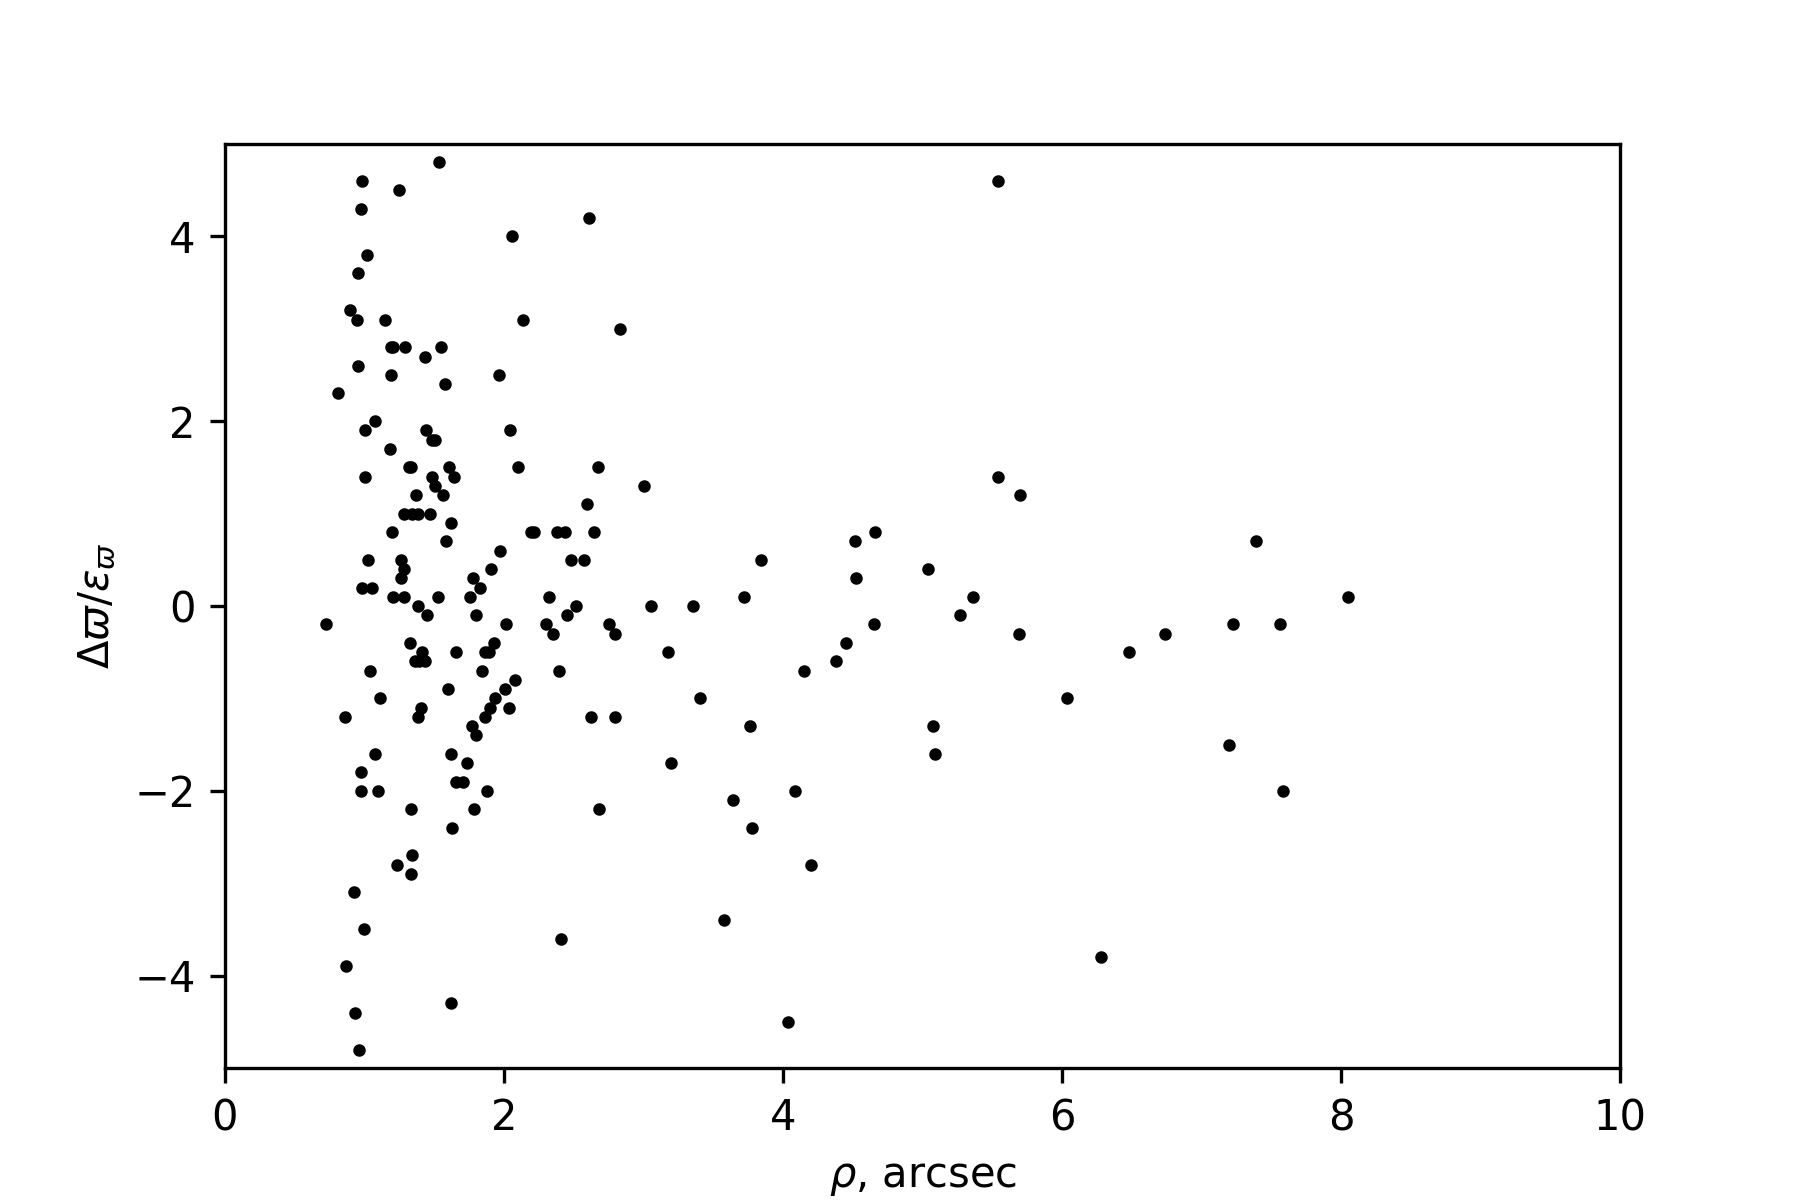
\includegraphics[width=0.7\textwidth]{delta_pi-vs-rho}
\end{center}
\end{frame}
%%%%%%%%%%%%%%%%%%%%%%%%%%%%%%%%%%%%%%%%%%%%%%%%%%%%%%%%%%%%%%%%%%%%%%%%%%%%%%%%%%%%%%%%%%%%%%%%%%%%%%%%%%%%%%%%%%%%%%%%%%%%%%%%%%%%%%%%%%%%%%%%%%%%%%%%%%%%%%


\begin{frame}
\frametitle{Угловые разделения}
\begin{center}
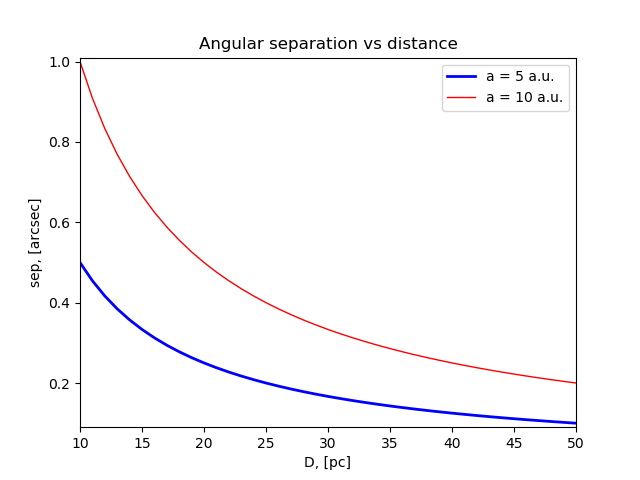
\includegraphics[width=0.6\textwidth]{separation-vs-distance}
\end{center}
%{\tiny Поиск и определение динамических параметров маломассивных двойных систем -- актуальная задача для наблюдателей. Для широкого класса подобных объектов $\rho<FWHM$.}
\end{frame}



\begin{frame}%{{\tiny \it Поиск ``легких'' двойных систем активно производится...}}
\frametitle{Альтернативные методы}
\begin{columns}
\column{0.3\textwidth}
	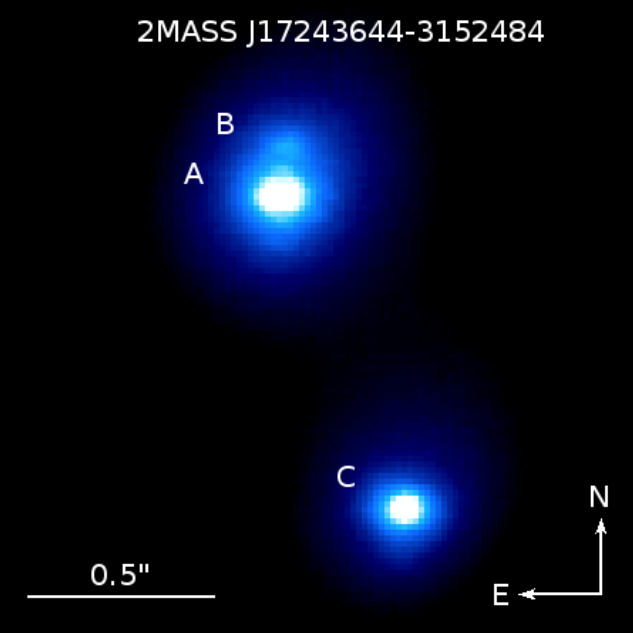
\includegraphics[width=0.99\columnwidth]{lucky-imaging-example}
	{\footnotesize Lucky imaging\\ Janson et al., 2017}
\column{0.7\textwidth}
	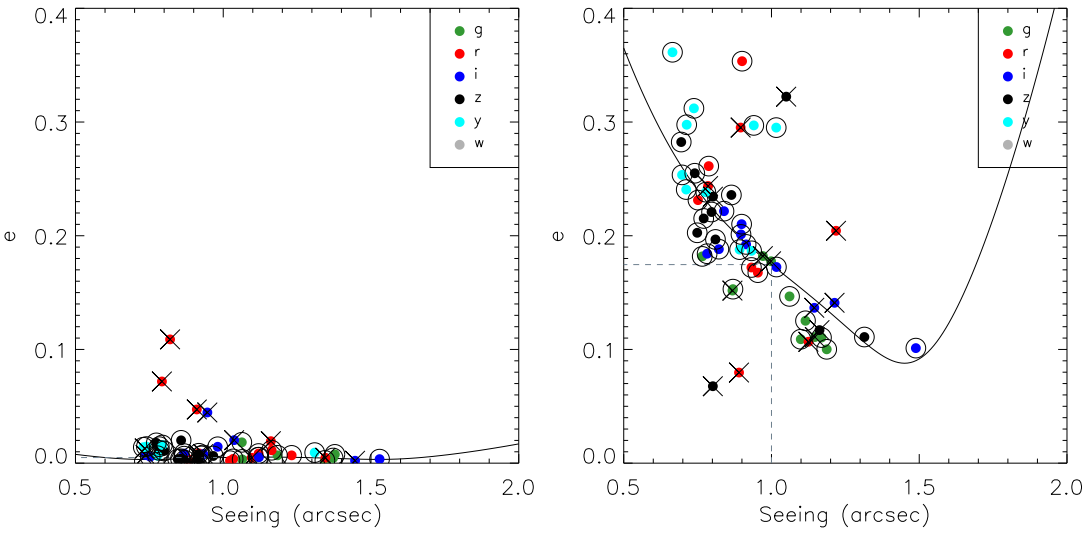
\includegraphics[width=0.99\columnwidth]{Deacon-ellipticity}
    {\footnotesize Эллиптичность изображения, Deacon et al., 2017\\ 
    Слева --- одиночная звезда, справа --- двойная.}
\end{columns}
\end{frame}



\begin{frame}%{{\tiny \it Зачем нужны маломассивные компоненты двойных систем?}}
\frametitle{Актуальность исследования}
{\small
\begin{itemize}
\item Для тестирования моделей звездообразования необходима репрезентативная выборка двойных и кратных звезд, содержащих маломассивные компоненты.
\item Миссия Gaia обеспечивает прогресс исследований в этом направлении, но ``не закрывает'' проблему.
\item Естественный подход -- применение методов высокого разрешения.
\item Наблюдения в рамках этой задачи ведутся на инструментах метрового класса в разных обсерваториях мира. 
\end{itemize}
}
\end{frame}

%%%%%%%%%%%%%%%%%%%%%%%%%%%%%%%%%%%%%%%%%%%%%%%%%%%%%%%%%%%%%%%%%%%%%%%%%%%%%%%%%%%%%%%%%%%%%%%%%%%%%%%%%%%%%%%%%%%%%%%%%%%%%%%%%%%%%%%%%%%%%%%%%%%%%%%%%%%%%%


\begin{frame}
\frametitle{Быстрые звезды}
\begin{columns}
\column{0.7\textwidth}
	%\includemovie{1cm}{1cm}{images/Barnard.gif}
	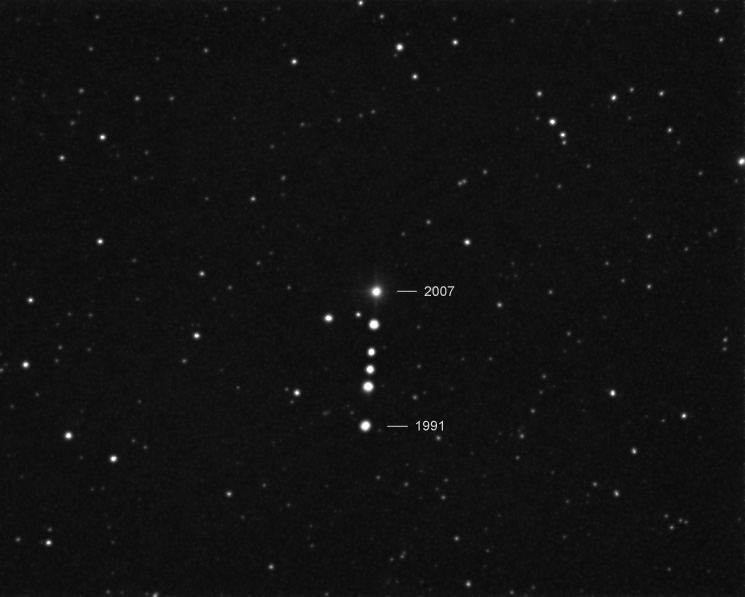
\includegraphics[width=0.99\columnwidth]{barnards}
	{\footnotesize Э. Барнард, 1916 \\ $\mu = 10.358~''/yr$, \\ $D = 1.8$ pc, \\ $V_r > 110$ км/сек}
\column{0.3\textwidth}
	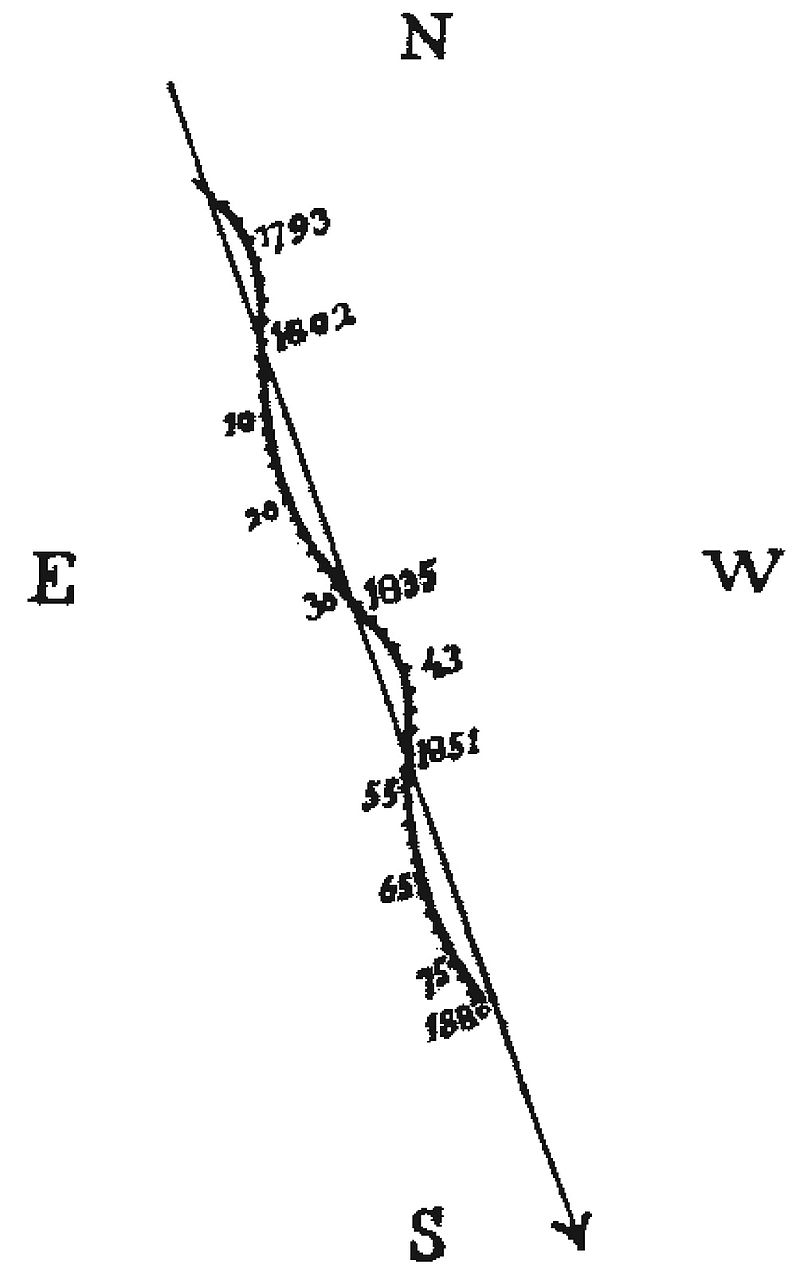
\includegraphics[width=0.99\columnwidth]{Sirius}
    {\footnotesize Ф.~Бессель, 1844}
\end{columns}
\end{frame}


\begin{frame}%{{\tiny \it $\Delta\mu$-двойные в FK6}}
\frametitle{$\Delta\mu$-двойные в FK6}
\begin{columns}
	\column{0.5\textwidth}
		%\begin{center}
		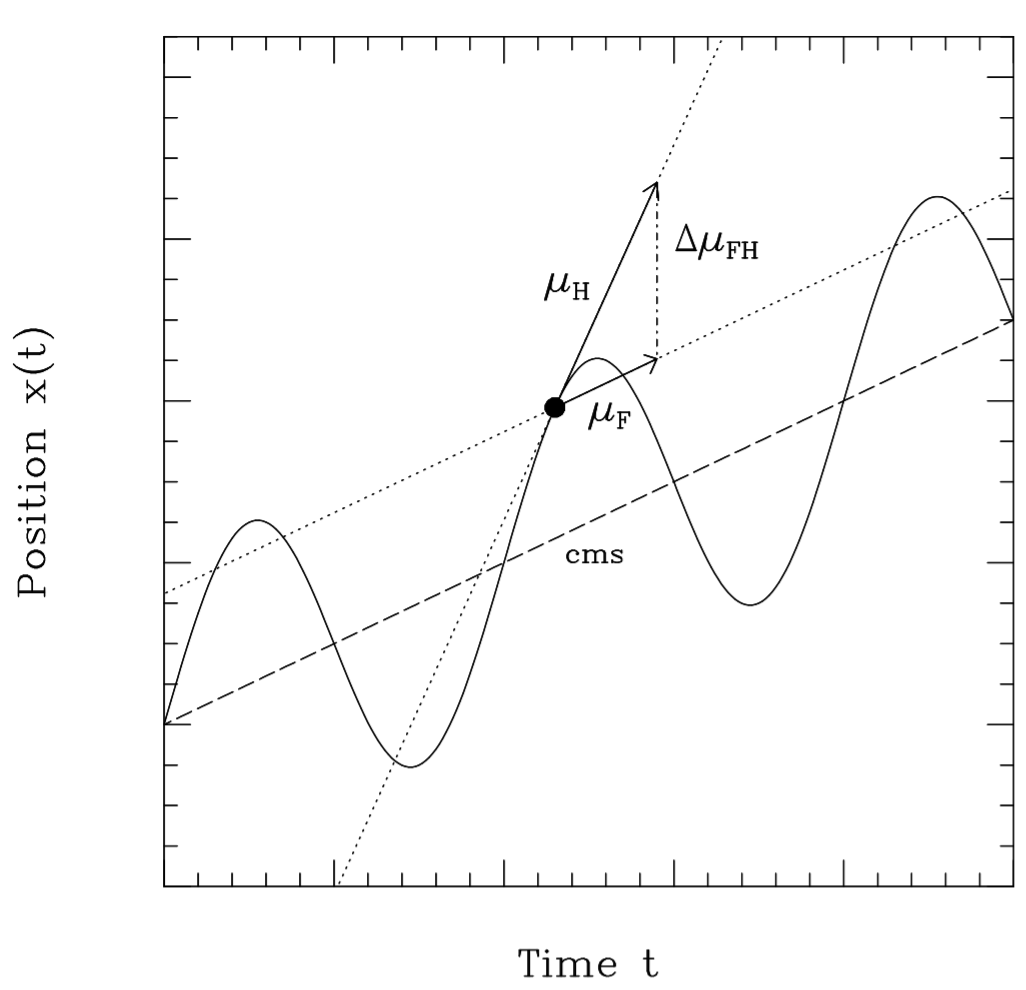
\includegraphics[width=0.99\columnwidth]{Wielen-idea}
		%\end{center}
	\column{0.5\textwidth}
		{\footnotesize Wielen et al., 1999:}\\
		{\footnotesize $F^{2}_{0H} =\left(\frac{\Delta\mu_{0H,\psi}}{\epsilon_{\Delta\mu_{0H,\psi}}}\right)^{2}+\left(\frac{\Delta\mu_{0H,\bar{\psi}}}{\epsilon_{\Delta\mu_{0H,\bar{\psi}}}}\right)^{2}$}\\
		{\footnotesize D < 100 pc в основном}\\
\end{columns}
\end{frame}


\begin{frame}%{{\tiny \it $\Delta\mu$-двойные в FK6}}
\frametitle{$\Delta\mu$-двойные в FK6}
\begin{columns}
	\column{0.5\textwidth}
		%\begin{center}
		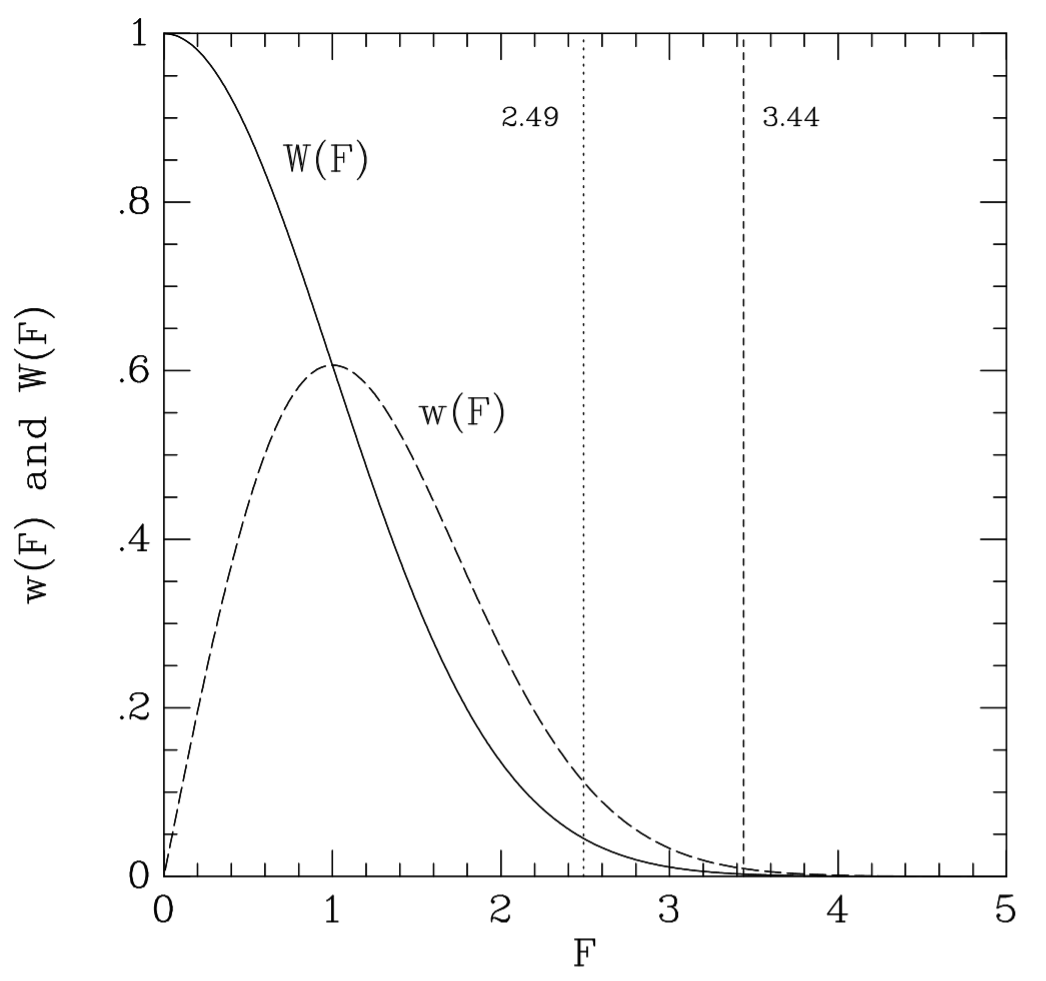
\includegraphics[width=0.99\columnwidth]{Wielen-Ww}
		%\end{center}
	\column{0.5\textwidth}
		{\footnotesize $W(F) = e^{-F^2_{0H}/2}$}\\
		{\footnotesize $w(F) = -\frac{dW(F)}{dF} = F_{0H}\,e^{-F^2_{0H}/2}$}\\
		{\footnotesize F > 3.44 ($3\sigma$) --- $\Delta\mu$-двойные}\\
		{\footnotesize F < 2.49 ($2\sigma$) --- одиночные}\\
		{\footnotesize В результате:\\ \approx 10\,\%  - $\Delta\mu$-двойные}\\
\end{columns}
\end{frame}

%%%%%%%%%%%%%%%%%%%%%%%
\begin{frame}%{{\tiny \it $\Delta\mu$-двойные среди близких карликов}}
\frametitle{Состоятельность задачи}
\begin{center}
{\footnotesize $D=25~pc, a=10~a.u.$}
\end{center}
\begin{columns}
\column{0.5\textwidth}
	\begin{center}
	{\footnotesize $M = 0.35M_\odot$}
	\end{center} 
	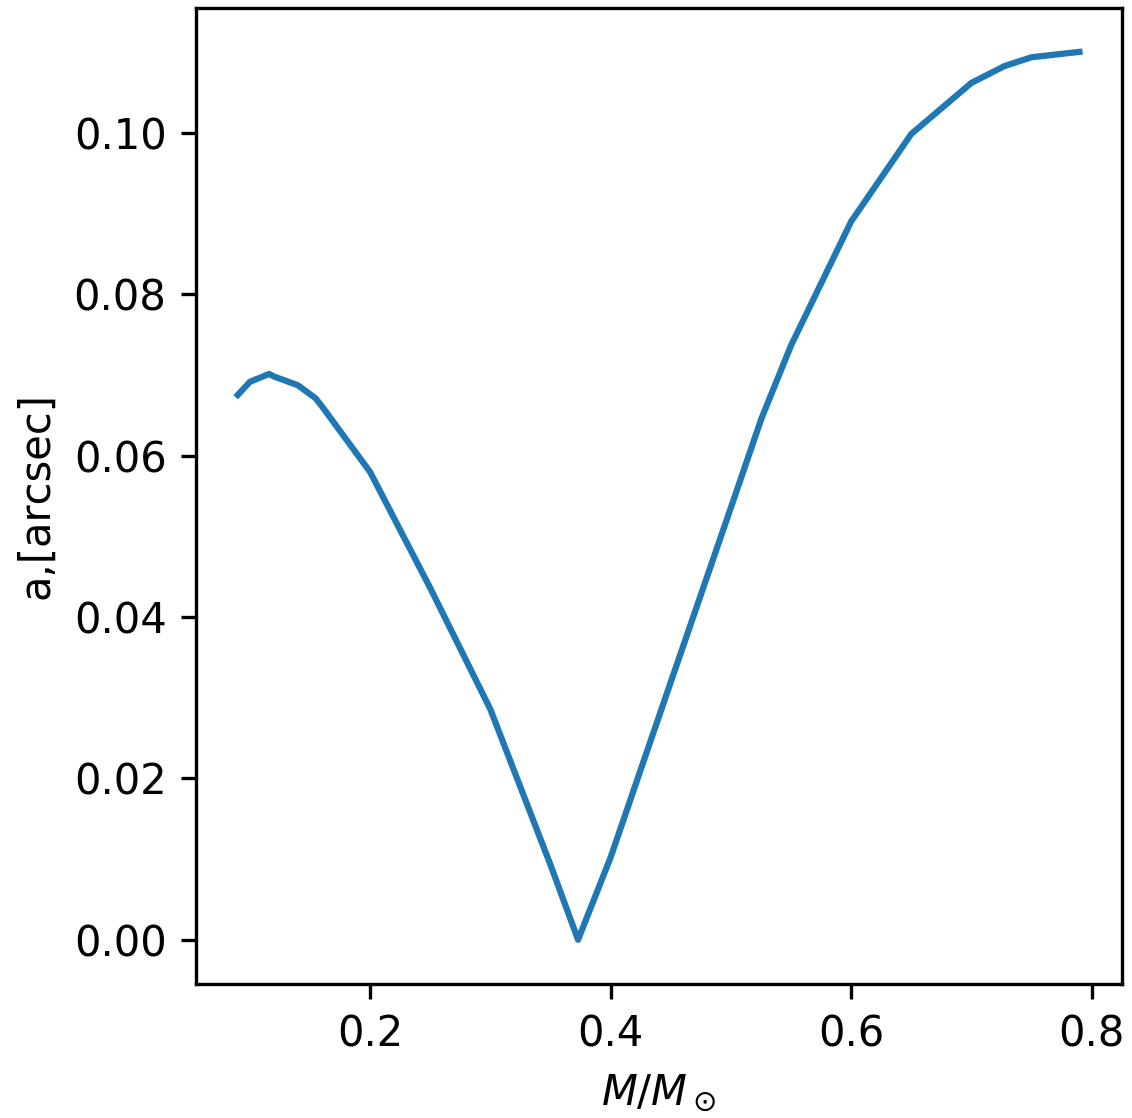
\includegraphics[width=0.99\columnwidth]{semiaxis_vs_mass035_10_25}
 \column{0.5\textwidth}
 \begin{center}
	{\footnotesize $M = 0.73M_\odot$}
	\end{center} 
	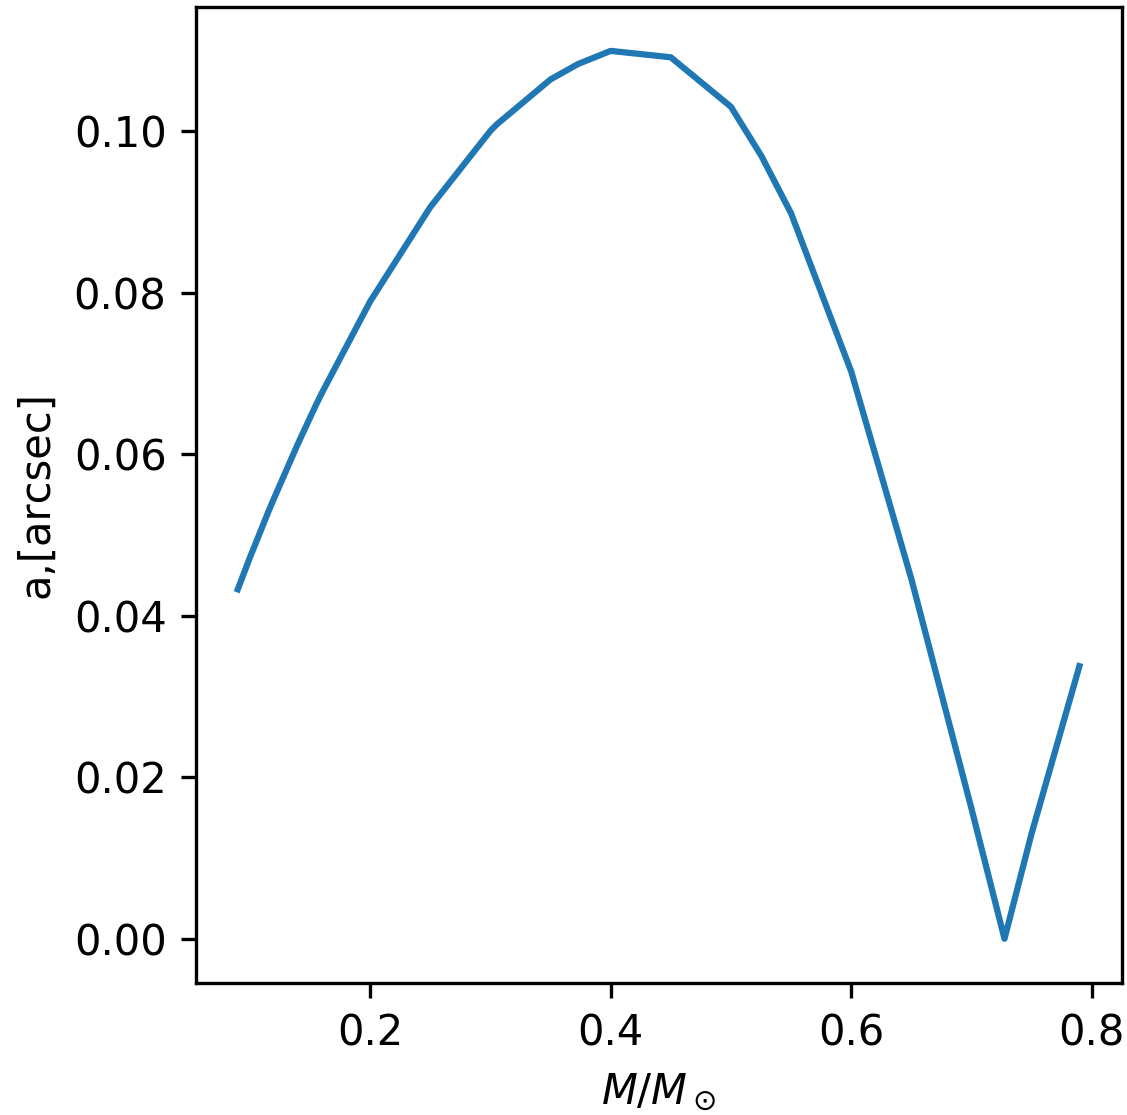
\includegraphics[width=0.99\columnwidth]{semiaxis_vs_mass073_10_25}
\end{columns}
%{\tiny Большая полуось видимой орбиты фотоцентра в зависимости от масс компонент. }
\\ 
\end{frame}



\begin{frame}%{{\tiny \it $\Delta\mu$-двойные среди близких карликов}}
\frametitle{Состоятельность задачи: {\small $\Delta\mu$-двойные}}
\begin{center}
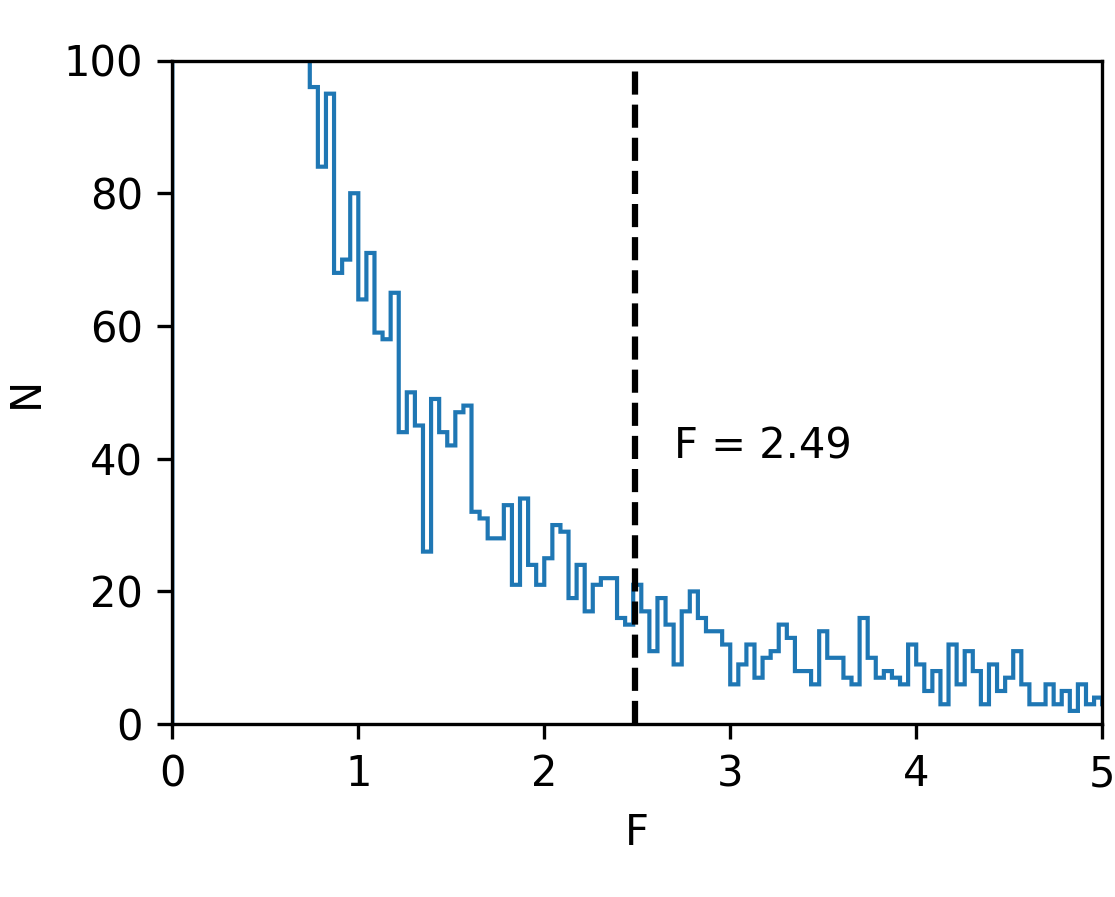
\includegraphics[width=0.7\textwidth]{F-hist}
\end{center}
\begin{center}
{\footnotesize \\ $D<50~pc$, функция масс --- Chabrier, 2005, распределение \textbf{a} --- Raghavan et al.,2010, результат: 1000 систем из 14\,000.}
\end{center}
\end{frame}


\begin{frame}%{{\tiny \it $\Delta\mu$-двойные среди близких карликов}}
\frametitle{Состоятельность задачи: {\small анализ изображений}}
\begin{center}
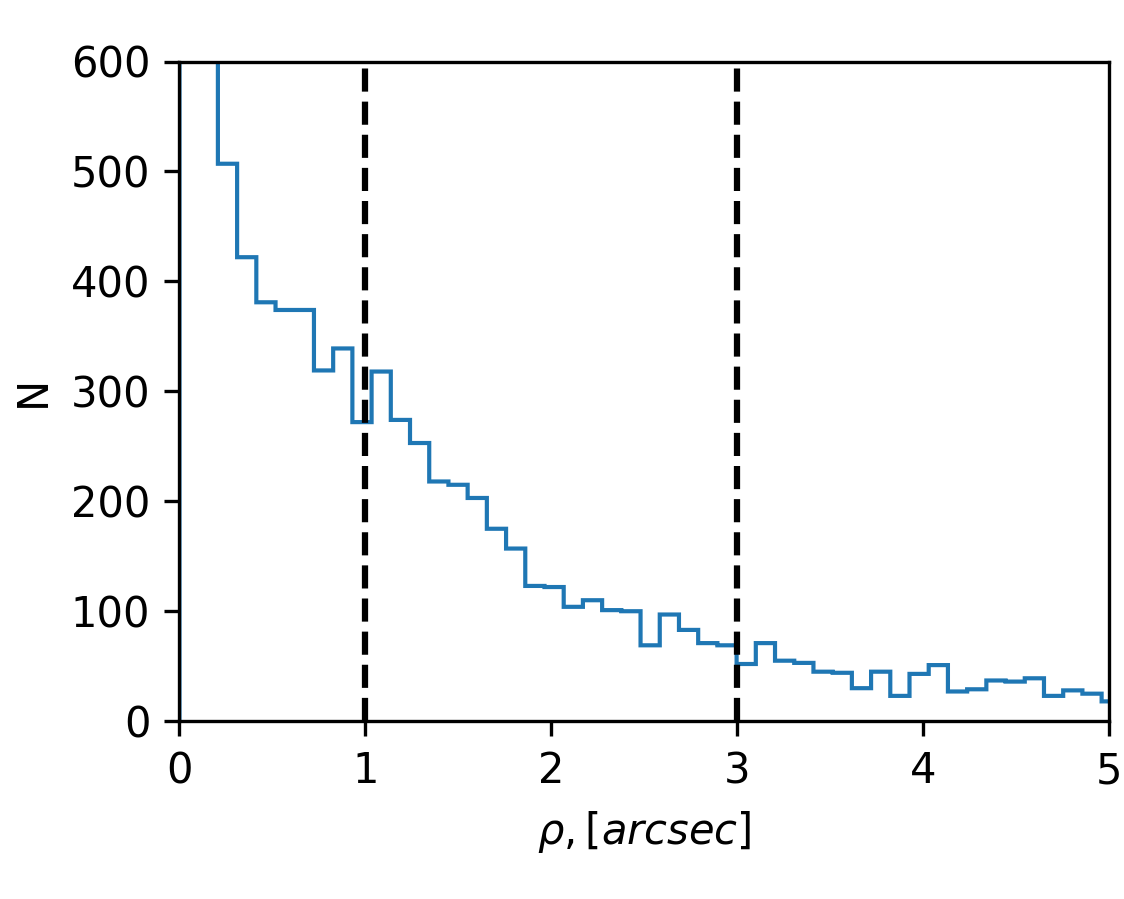
\includegraphics[width=0.7\textwidth]{rho-hist}
\end{center}
\begin{center}
{\footnotesize \\ Вертикальные линии - границы: $0.5\,FWHM<\rho<FWHM$, ожидаемый результат: до 20\,\% от популяции двойных систем.}
\end{center}
\end{frame}
%%%%%%%%%%%%%%%%%%%%%%%%%%%%%%%%%%%%%%%%%%%%%%%%%%----------------ХРУЦКАЯ----------------%%%%%%%%%%%%%%%%%%%%%%%%%%%%%%%%%%%%%%%%%%%%%%%%%%

\begin{frame}%{{\tiny \it $\Delta\mu$-двойные в Пулково: первая реализация}}
\frametitle{$\Delta\mu$-двойные в Пулково: {\small первый опыт}}
\begin{columns}
\column{0.5\textwidth}
	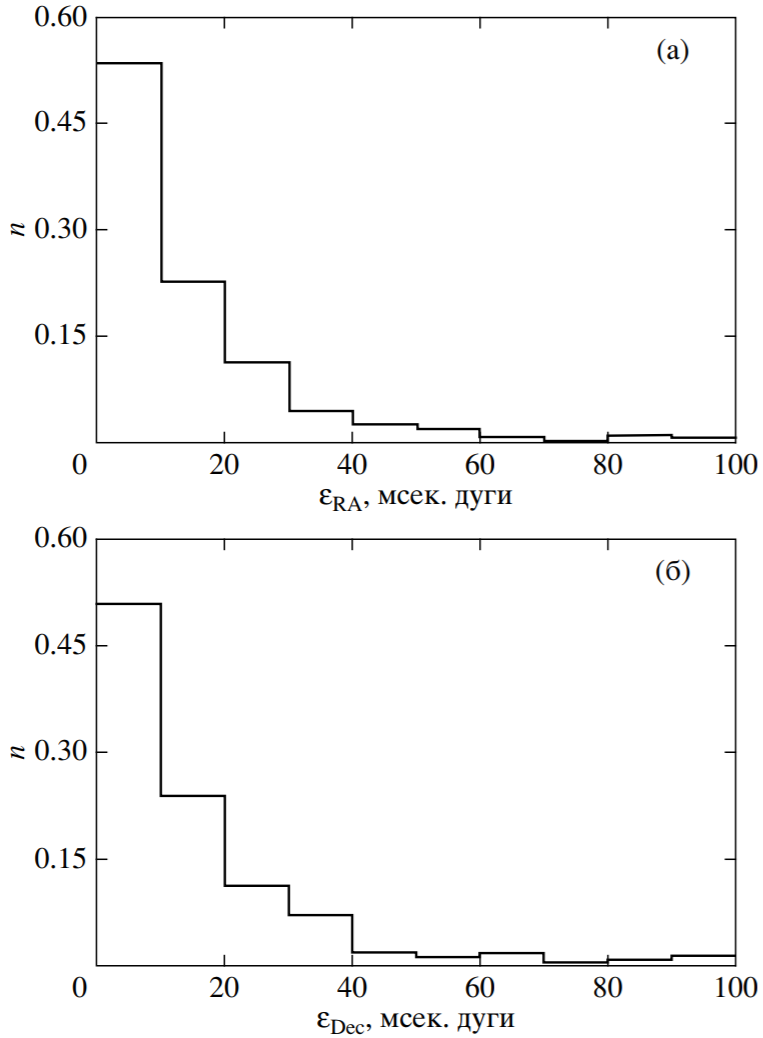
\includegraphics[width=0.8\columnwidth]{khrutskaya3}
 \column{0.5\textwidth}
	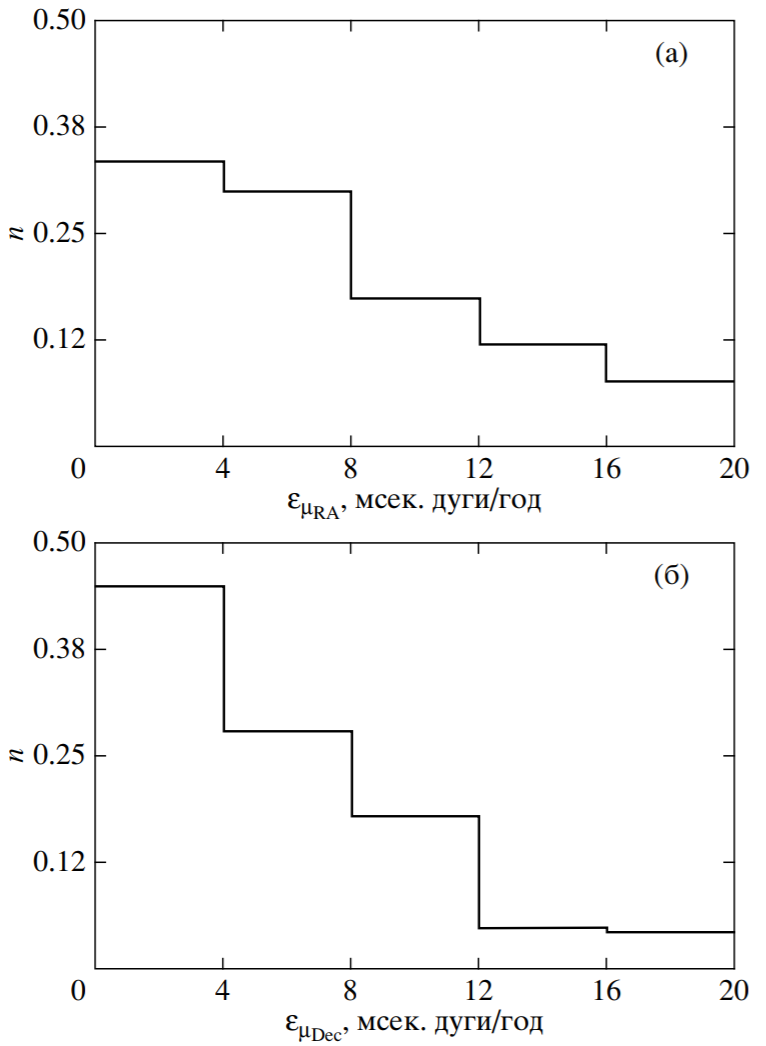
\includegraphics[width=0.8\columnwidth]{khrutskaya4}
\end{columns}
\begin{center}
{\scriptsize Khrutskaya et al., 2011: 414~объектов, $\mu > 300\,mas/yr$,  аппроксимация по профилю Лоренца, редукция в HCRF/UCAC3 положений Пулково, CMC14, M2000, 2MASS, SDSS DR7, результат: 70 звезд, 42 из них --- входят в WDS}
\end{center}
\end{frame}

%%%%%%%%%%%%%%%%%%%%%%%%%%%%%%%%%%%%%%%%%%%%%%%%%%----------------Shapelet----------------%%%%%%%%%%%%%%%%%%%%%%%%%%%%%%%%%%%%%%%%%%%%%%%%%%
\begin{frame}
\frametitle{Shapelet разложение}
{\footnotesize Разложение по базисным функциям:}\\
{\footnotesize $\phi_n(x) = \left(2^n\sqrt{\pi}n!\right)^{-\frac{1}{2}}H_n(x)e^{-\frac{x^2}{2}}$}\\
{\tiny $H_n(x)$ --- полином Эрмита порядка n, x --- независимая вещественная переменная}\\[10pt]
{\footnotesize Для двумерного случая:}\\
{\footnotesize $B_{n_1,n_2}(\beta,x,y,x_{ph},y_{ph}) = \beta^{-1}\cdot\phi_{n_1}\left(\frac{x-x_{ph}}{\beta}\right)\cdot\phi_{n_2}\left(\frac{y-y_{ph}}{\beta}\right)$}\\
{\tiny $\beta$ --- характерный размер изображения}\\[10pt]
{\footnotesize Изображение:}\\
{\footnotesize $I(x,y) = I_{bgr}+\sum_{n_1,n_2=0}^{\infty}f_{n_1,n_2}\cdot B_{n_1,n_2}(\beta,x,y,x_{ph},y_{ph})$}\\
{\tiny $f_{n_1,n_2}$ --- коэффициенты шейплет-разложения соответствующих порядков $n_1$, $n_2$.}\\[15pt]
{\footnotesize (Refregier, 2001)}
\end{frame}


\begin{frame}
\frametitle{Shapelet разложение}
{\footnotesize Поток:}\\
{\tiny $F = \sqrt{\pi} \beta \sum^{even}_{n_1,n_2} \sqrt{2^{2-n_1-n_2}C^{\frac{n_1}{2}}_{n_1}C^{\frac{n_2}{2}}_{n_2}}f_{n_1,n_2}$}\\[15pt]
{\footnotesize Положение фотоцентра:}\\
{\scriptsize $x_1^f = \sqrt{\pi} \beta^2 F^{-1} \sum^{odd}_{n_1}\sum^{even}_{n_2} \sqrt{(n_1+1)2^{2-n_1-n_2}C^{\frac{n_1+1}{2}}_{n_1+1}C^{\frac{n_2}{2}}_{n_2}}f_{n_1,n_2}$}\\[10pt]
{\scriptsize $x_2^f = \sqrt{\pi} \beta^2 F^{-1} \sum^{even}_{n_1}\sum^{odd}_{n_2} \sqrt{(n_2+1)2^{2-n_1-n_2}C^{\frac{n_1}{2}}_{n_1}C^{\frac{n_2+1}{2}}_{n_2+1}}f_{n_1,n_2}$}\\[15pt]
{\tiny $even$ --- суммирование по четным индексам $n_1$ и $n_2$, $odd$ --- по нечетным,\\ $C^p_q$ --- биномиальный коэффициент для соотв. индекса.}\\[15pt]
{\footnotesize (Refregier, 2001)}
\end{frame}


\begin{frame}
\frametitle{Shapelet разложение}
\begin{center}
\begin{columns}
\column{0.5\textwidth}
	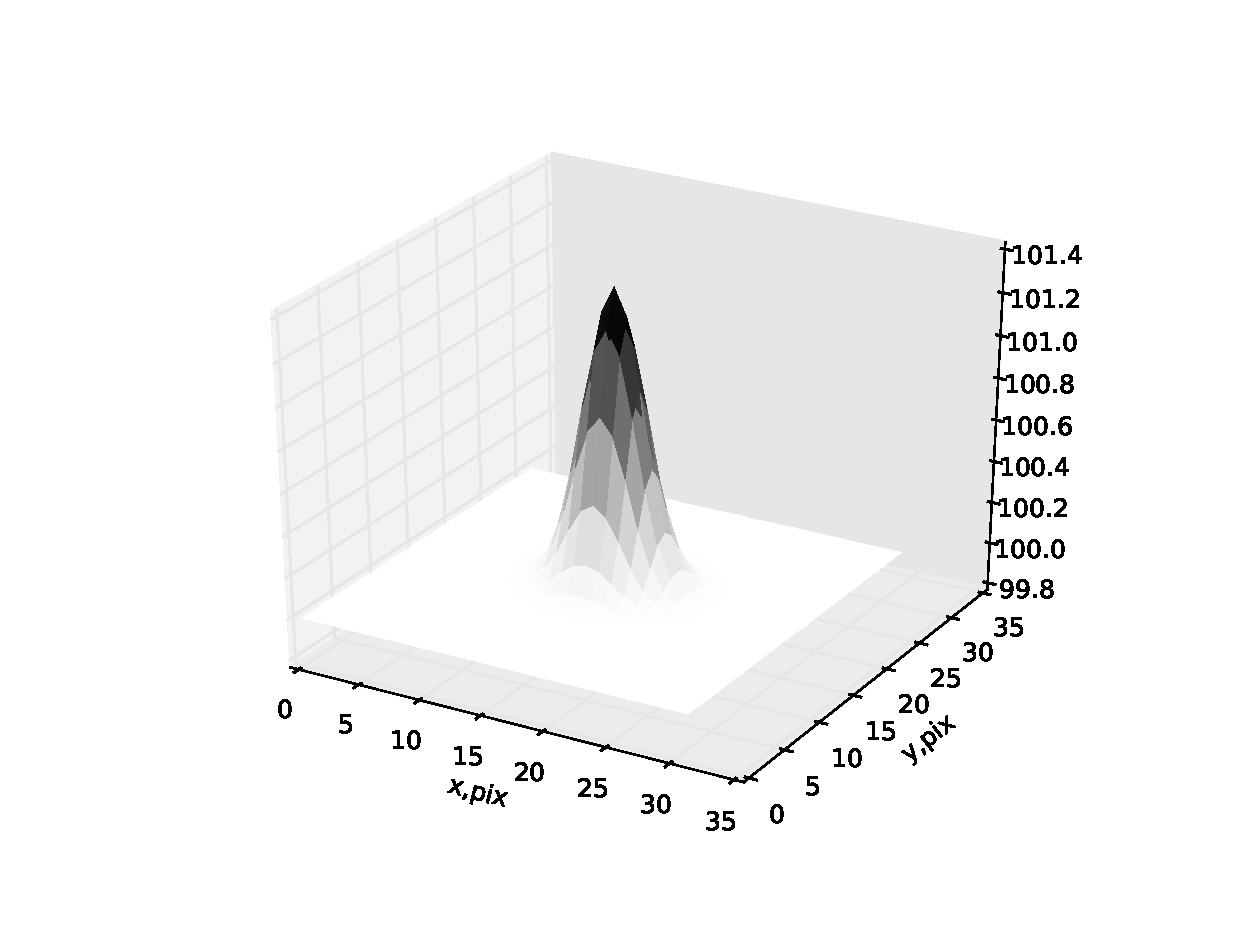
\includegraphics[width=0.7\columnwidth]{stimg_0}
	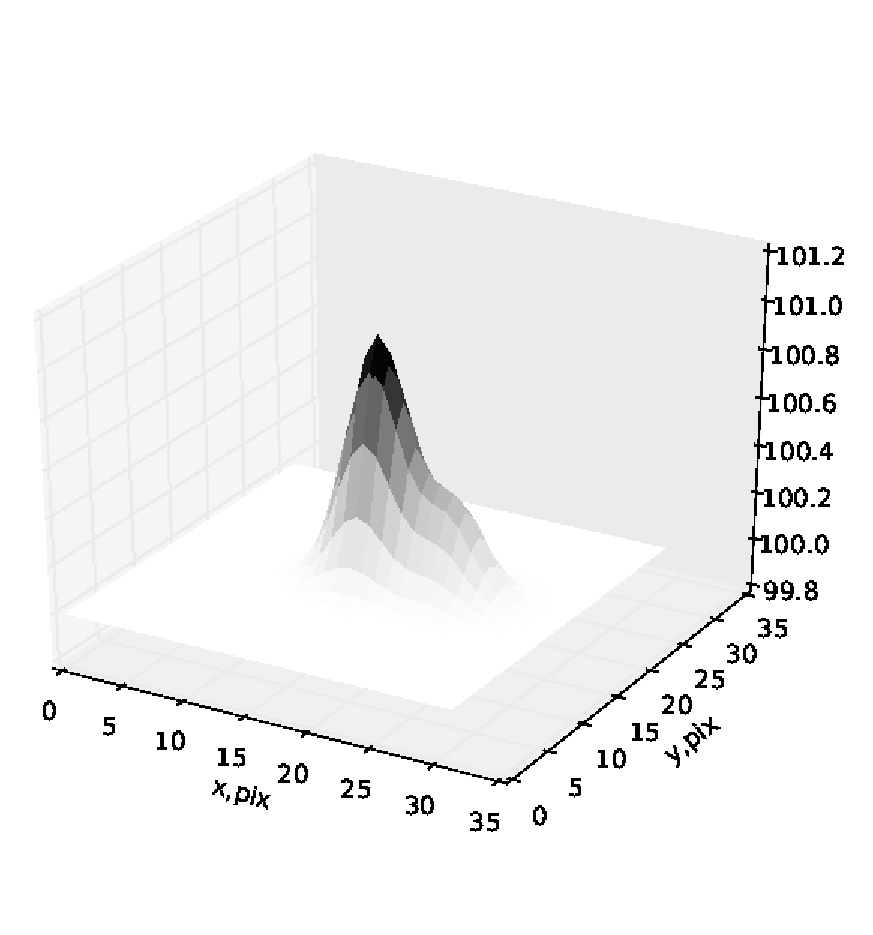
\includegraphics[width=0.7\columnwidth]{stimg_6}
\column{0.5\textwidth}
	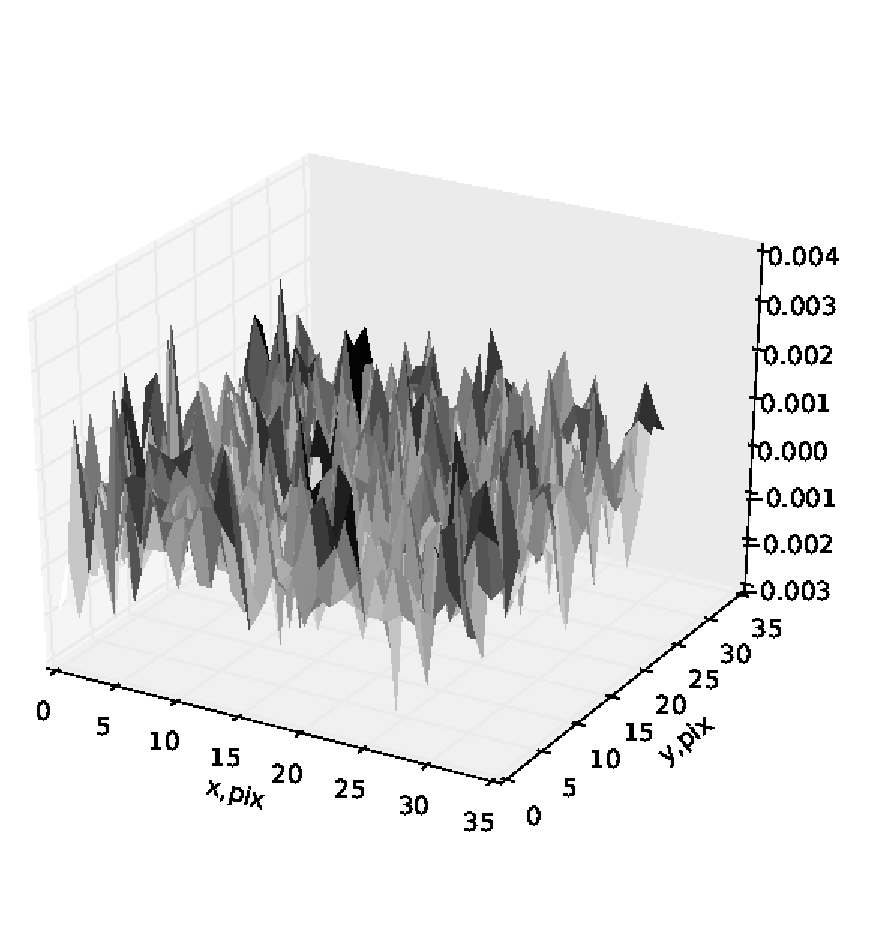
\includegraphics[width=0.7\columnwidth]{res_0}
	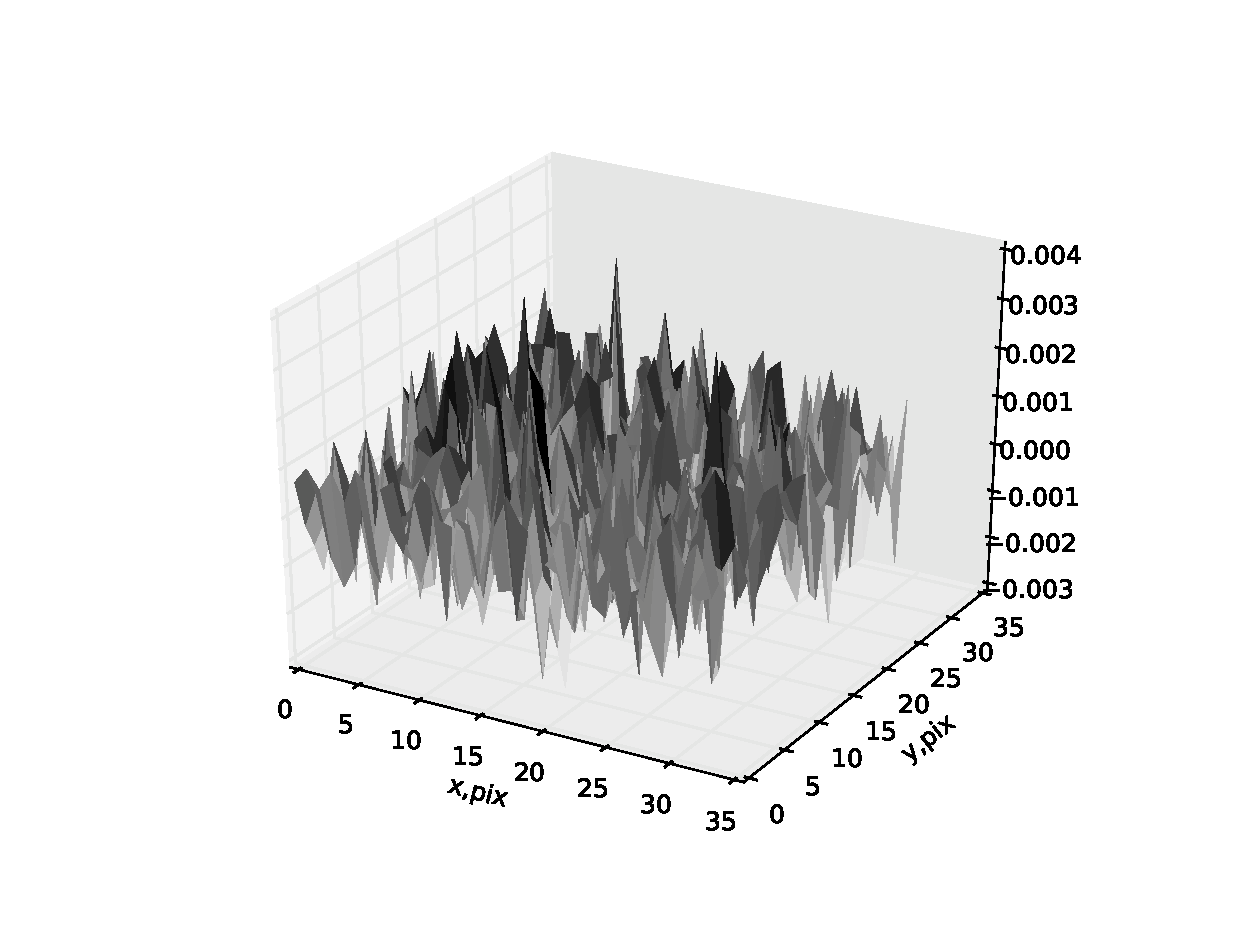
\includegraphics[width=0.7\columnwidth]{res_6}
\end{columns}
\end{center}
\end{frame}


\begin{frame}%{{\tiny Квадрупольные моменты}}
\frametitle{Квадрупольные моменты}
{\small
\begin{align*}
  q_{xx} & = F^{-1} \sqrt{\pi} \beta^3 \sum^{even}_{n_1,n_2} (1+2n_1) \sqrt{2^{2-n_1-n_2}C^{\frac{n_1}{2}}_{n_1}C^{\frac{n_2}{2}}_{n_2}}f_{n_1,n_2} \\
  \vspace{5mm}
  q_{yy} & = F^{-1} \sqrt{\pi} \beta^3 \sum^{even}_{n_1,n_2} (1+2n_2) \sqrt{2^{2-n_1-n_2}C^{\frac{n_1}{2}}_{n_1}C^{\frac{n_2}{2}}_{n_2}}f_{n_1,n_2} \\
  \vspace{5mm}
  q_{xy} & = F^{-1} \sqrt{\pi} \beta^3 \sum^{odd}_{n_1,n_2} \sqrt{(n_1+1)(n_2+1)2^{2-n_1-n_2}C^{\frac{n_1+1}{2}}_{n_1+1}C^{\frac{n_2+1}{2}}_{n_2+1}}f_{n_1,n_2} 
\end{align*}
}
\end{frame}


\begin{frame}
\frametitle{Эллиптичность и асимметрия}
\begin{center}
{\small
\begin{align*}

\left[e_1,~e_2\right] = \left[\frac{q_{xx}-q_{yy}}{q_{xx}+q_{yy}},~\frac{q_{xy}}{q_{xx}+q_{yy}}\right],\: e = \sqrt{e_1^2+e_2^2}\\[15pt]
A = F^{-1}\cdot \sum_{pixels} |I(x,y)-I(x,y)^{180}|

\end{align*}
}
\end{center}
{\footnotesize
	Эллиптичность вычисляется через квадрупольные моменты, индекс асимметрии --- через поворот исходного изображения $I(x,y)$ на $180^\circ$.
}
\end{frame}

%%%%%%%%%%%%%%%%%%%%%%%%%%%%%%%%%%%%%%%%%%%%%%%----------------3.2.1 - 3.2.2----------------%%%%%%%%%%%%%%%%%%%%%%%%%%%%%%%%%%%%%%%%%%%%%%%
\begin{frame}%{{\tiny \it $\Delta\mu$-двойные в Пулково: первая реализация}}
\frametitle{$\Delta\mu$-двойные среди близких карликов\\{\small формирование списка}}
\begin{columns}
\column{0.4\textwidth}
	\includegraphics[width=1.2\columnwidth]{fig1_a.eps}
 \column{0.6\textwidth}
{\scriptsize 
\begin{itemize}
\item[] 1972 звезды до $17^m$ в зоне склонения $+30^{\circ}$~--~$+70^{\circ}$ из LSPM\\[10pt]
\item[] у 1507 $\mu > 300$~mas/yr\\[10pt]
\item[] наблюдения PNA (D\,=\,300\,мм, F\,=\,3500\,мм) 2008\,--\,2015\\[10pt]
\item[] SDSS DR12 (Alam et al., 2015), 2MASS (Cutri et al., 2003), WISE (Wright et al., 2010, холодная серия)\\[10pt]
\item[]STScI DSS (Lasker et al., 1998) - сканы Паломарского обзора POSSI-O, POSSII-J\\[10pt]
%\item $\mu_{inst}$ - ПЗС-кадры с Нормального астрографа, SDSS, WISE, 2MASS (1998~--~2015).
%\item $\mu_{inst}$ - Палаллактические серии с 26-дюймового рефрактора.
%\item $\mu_{mean}$ - Оцифрованные астронегативы (1950~--~2000).
\end{itemize}
В итоге: $1308$ звезд от $10^m$ до $17^m$
}
\end{columns}
\end{frame}

%%%%%%%%%%%%%%%%%%%%%%%%%%%%%%%%%%%%%%%%%%%%%%%%%%----------------3.2.3----------------%%%%%%%%%%%%%%%%%%%%%%%%%%%%%%%%%%%%%%%%%%%%%%%%%%
\begin{frame}
\frametitle{$\Delta\mu$-двойные среди близких карликов\\{\small пиксельные координаты}}
\begin{center}
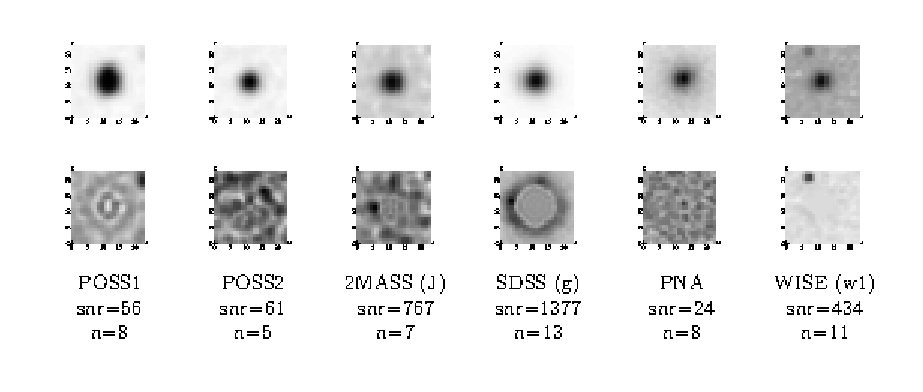
\includegraphics[width=0.9\textwidth]{fig3}
{\footnotesize Аппроксимация изображения J0753+5106 ($V_{mag}=14.2$),\\ размер области $24\,pix\,\times 24\,pix$.}
\end{center}
\end{frame}

%%%%%%%%%%%%%%%%%%%%%%%%%%%%%%%%%%%%%%%%%%%%%%%%%%----------------3.2.4----------------%%%%%%%%%%%%%%%%%%%%%%%%%%%%%%%%%%%%%%%%%%%%%%%%%%
\begin{frame}%{{\tiny \it $\Delta\mu$-двойные среди близких карликов. Итоги}}
\frametitle{$\Delta\mu$-двойные среди близких карликов\\{\small анализ систематических ошибок}}
\begin{center}
\begin{columns}
\column{0.5\textwidth}
	\includegraphics[width=1\columnwidth]{fig4a}
\column{0.5\textwidth}	
	\includegraphics[width=1\columnwidth]{fig4b}
\end{columns}
\end{center}
{\footnotesize Зависимость остаточных разносей координат от блеска и положения на кадре. Слева: PNA ($0.950''/pix$), справа: WISE (W1, $2.758''/pix$). }
\end{frame}


\begin{frame}%{{\tiny \it $\Delta\mu$-двойные среди близких карликов. Итоги}}
\frametitle{$\Delta\mu$-двойные среди близких карликов\\{\small анализ систематических ошибок}}
\begin{center}
\begin{columns}
\column{0.5\textwidth}
	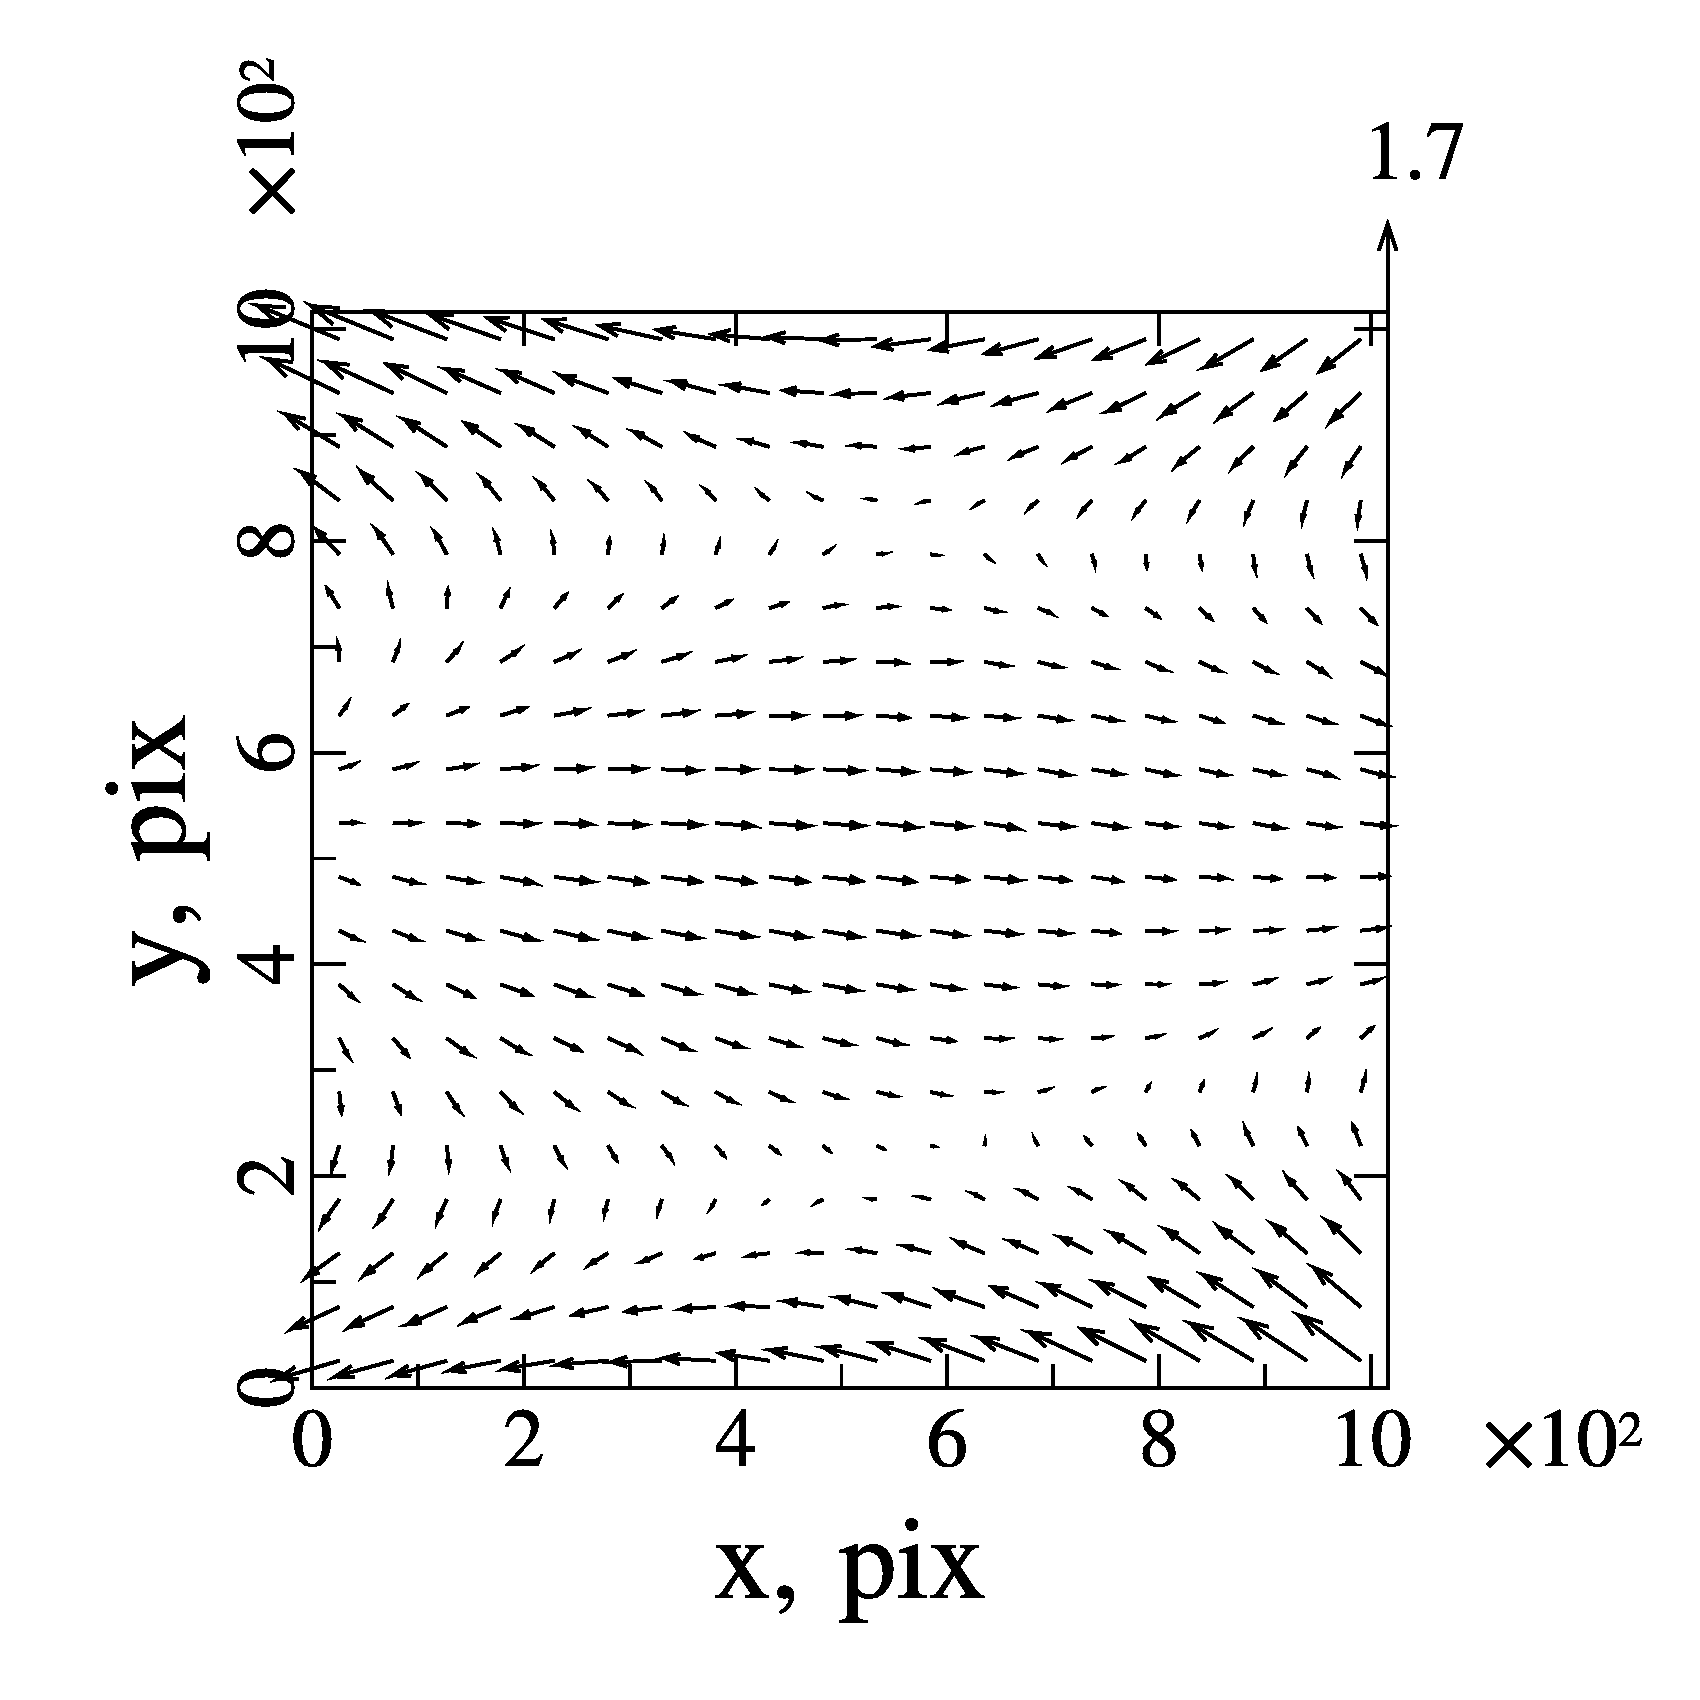
\includegraphics[width=0.9\columnwidth]{fig5a}
\column{0.5\textwidth}	
	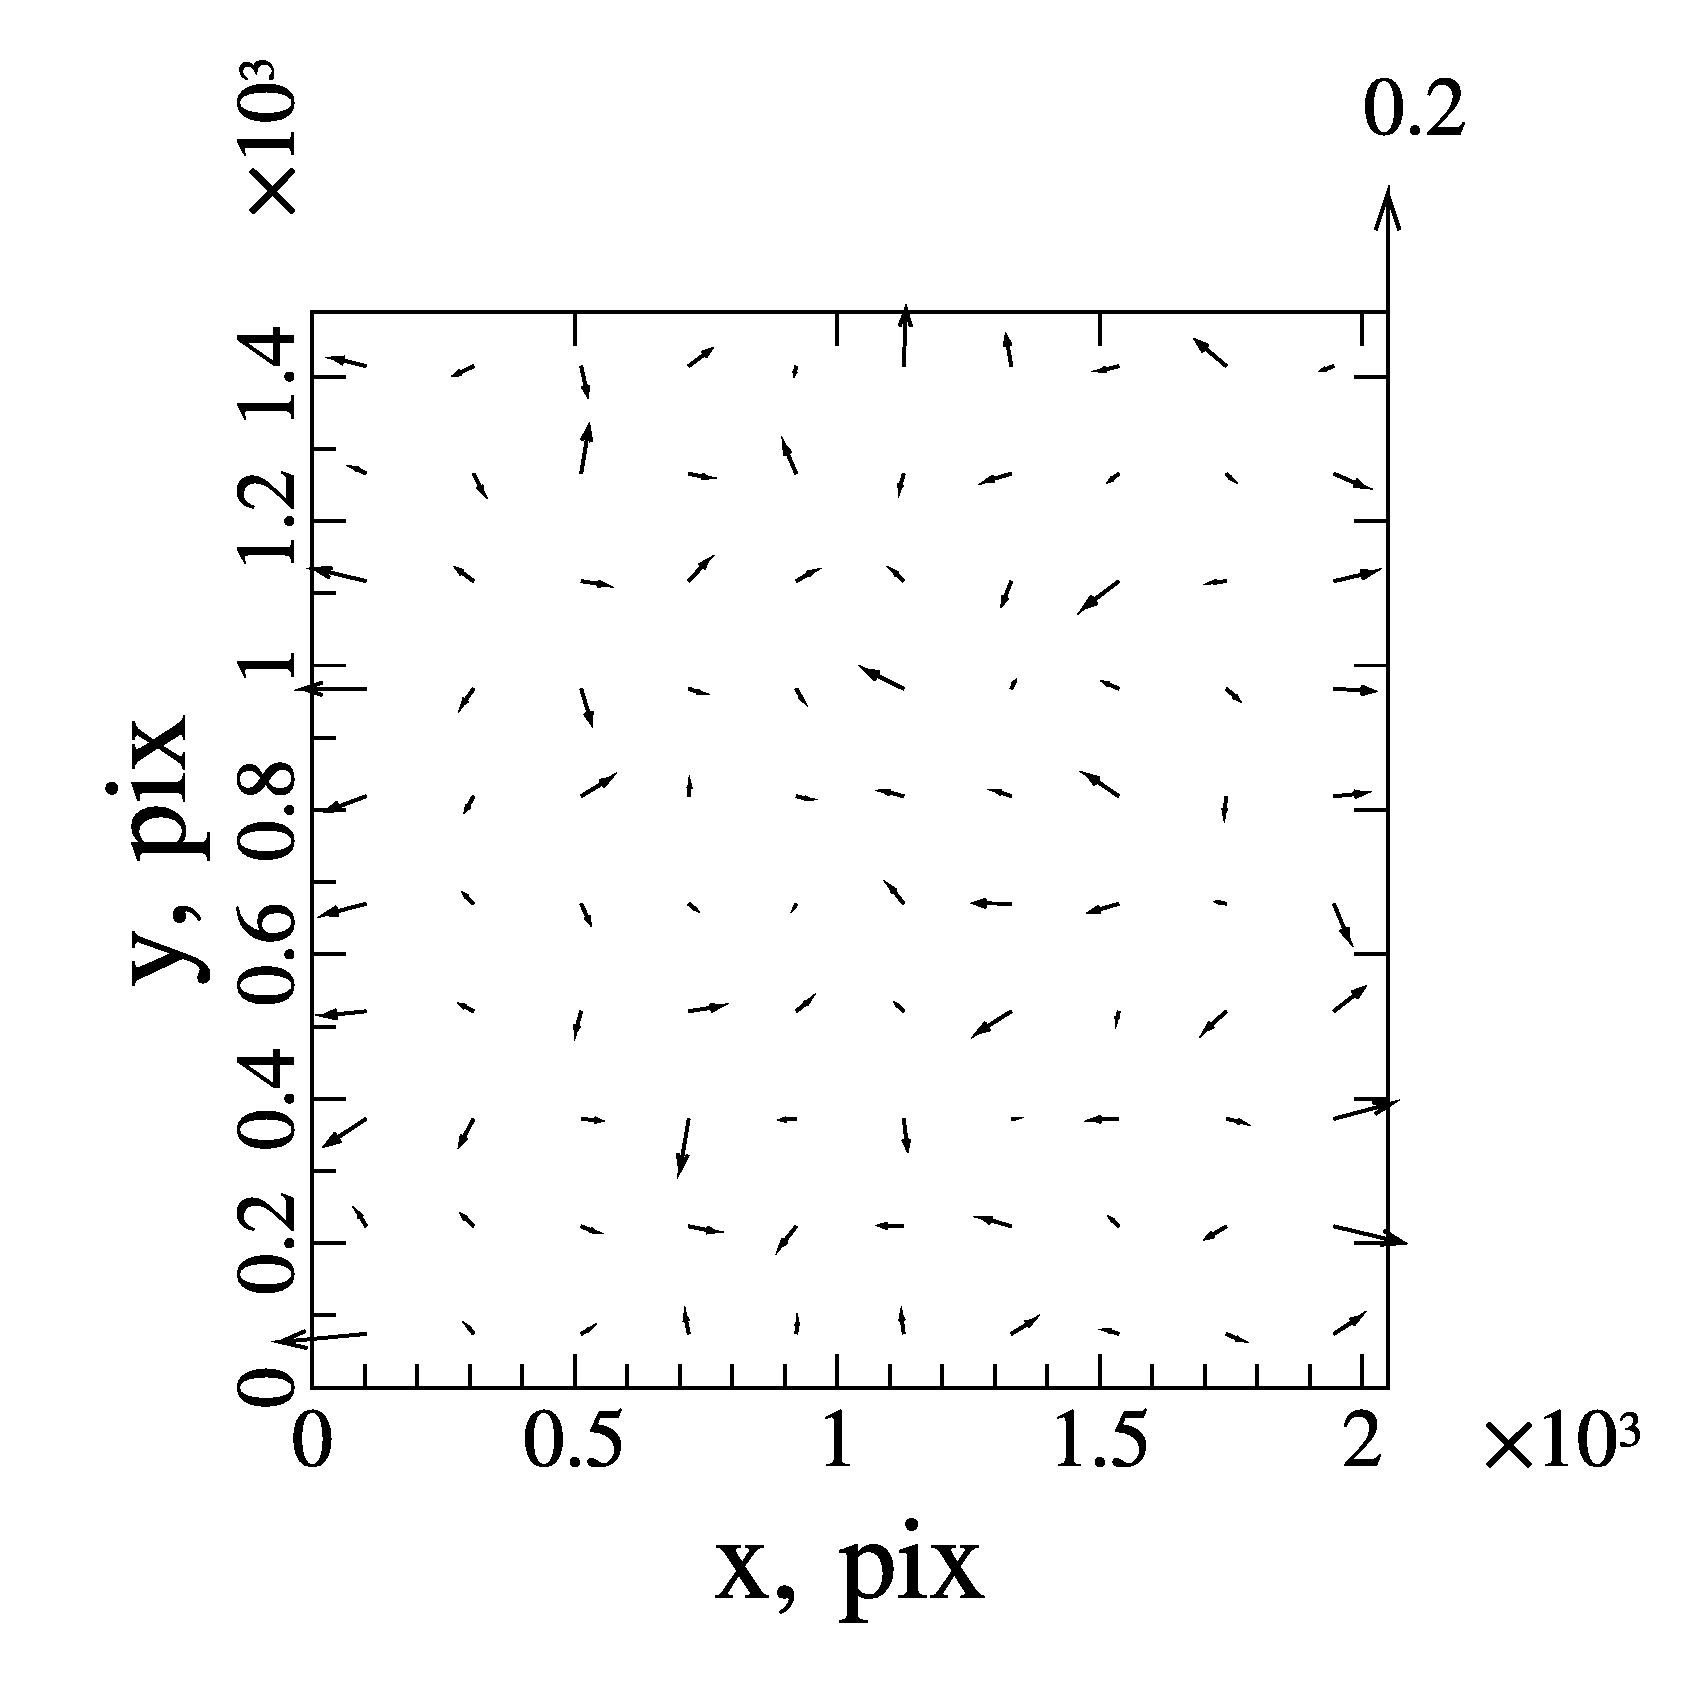
\includegraphics[width=0.9\columnwidth]{fig5b}
\end{columns}
\end{center}
{\footnotesize Остаточные разности пиксельных координат.\\ Слева: WISE (W1, $2.758''/pix$), справа: SDSS RD12 (r, $0.396''/pix$). }
\end{frame}
%%%%%%%%%%%%%%%%%%%%%%%%%%%%%%%%%%%%%%%%%%%%%%%%%%%%%%%----------------3.3--------------------%%%%%%%%%%%%%%%%%%%%%%%%%%%%%%%%%%%%%%%%%%%%%%%



\begin{frame}%{{\tiny \it $\Delta\mu$-двойные среди близких карликов. Итоги}}
\frametitle{$\Delta\mu$-двойные среди близких карликов}
\begin{columns}
\column{0.5\textwidth}
	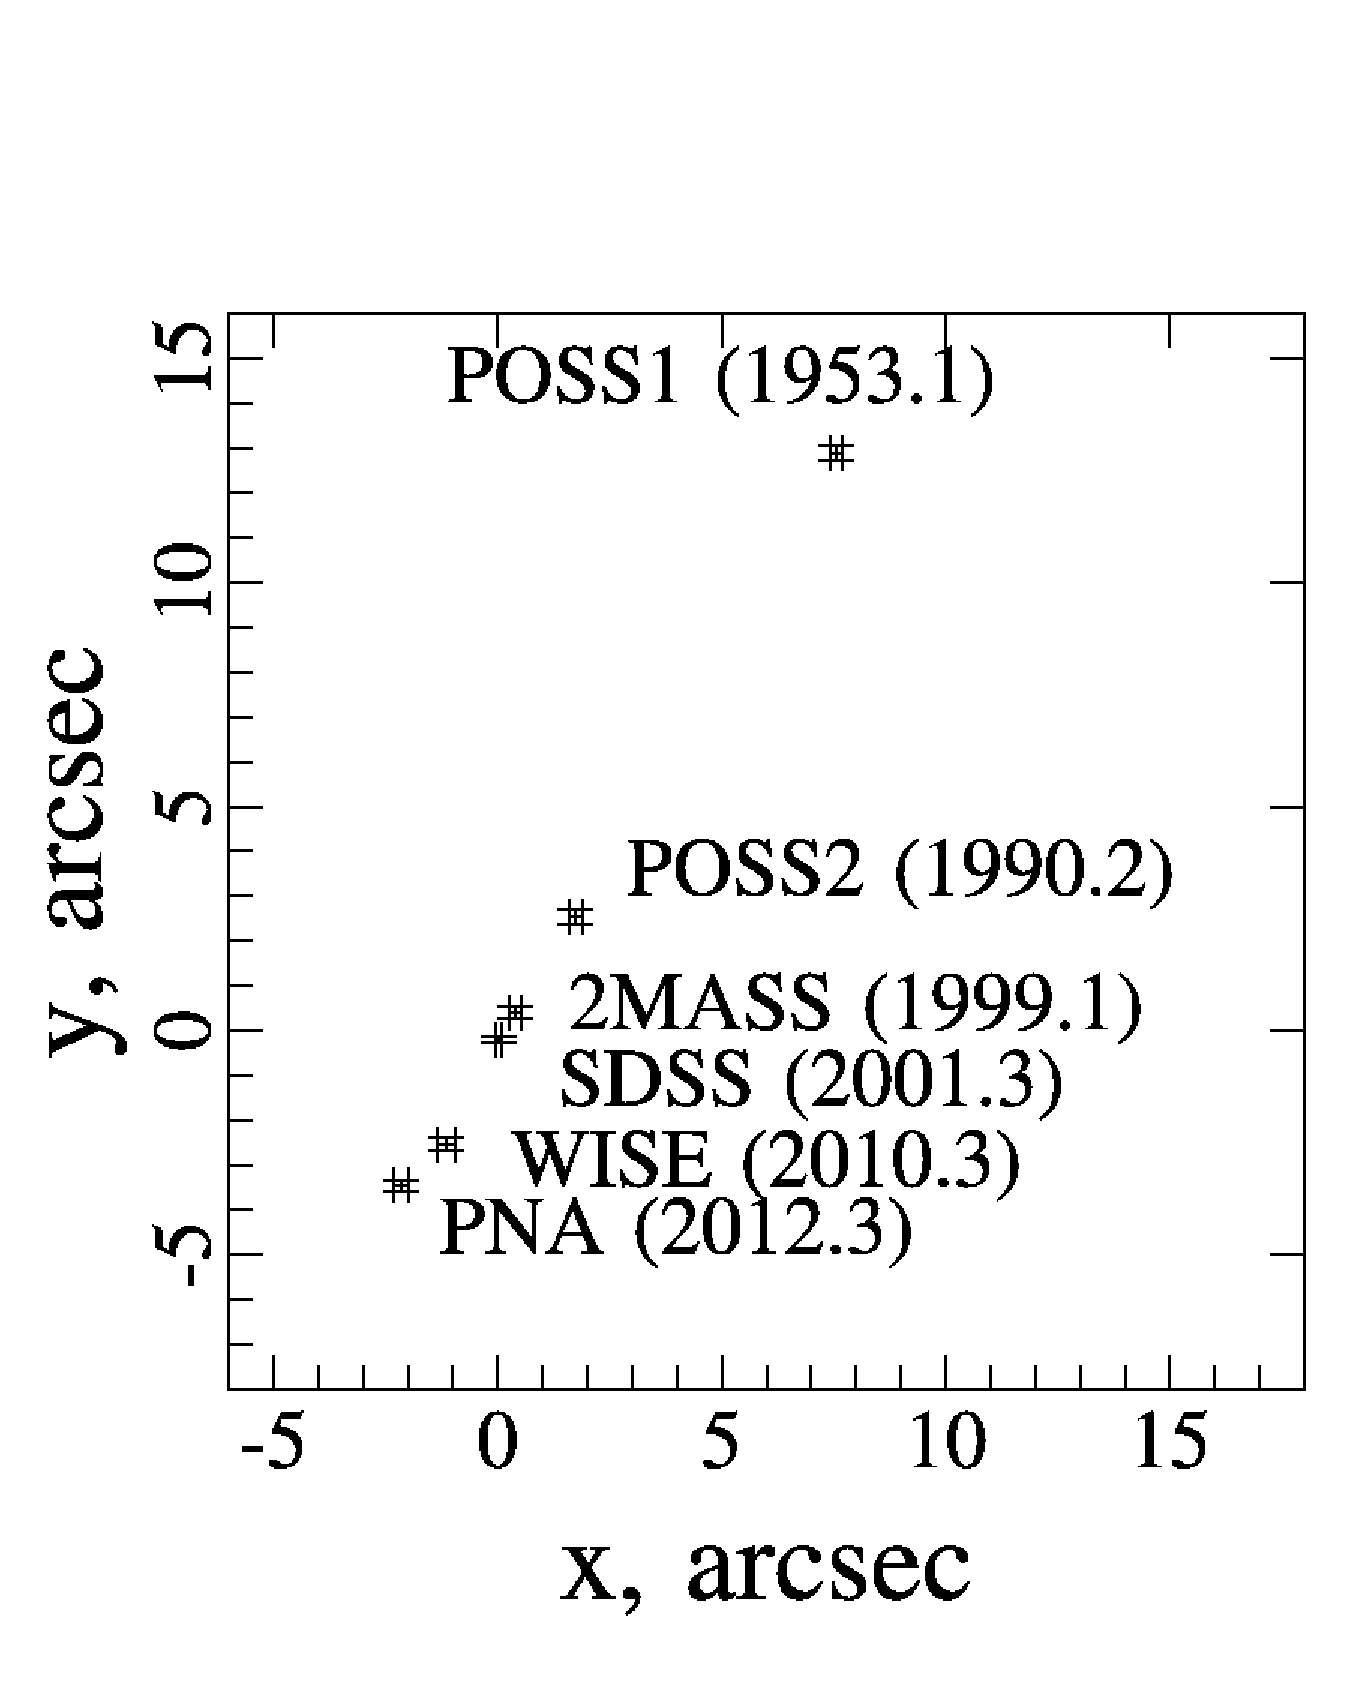
\includegraphics[width=1.1\columnwidth]{fig6}
\column{0.5\textwidth}	
	{\footnotesize
		J0838+4715, $\mu_{\alpha}=-158.1\pm2.6$~mas/yr, $\mu_{\delta}=-273.1\pm3.1$~mas/yr, $mean\;epoch = 1994.3328$, $V_{mag}=15.9$
	}
\end{columns}
\end{frame}


\begin{frame}%{{\tiny \it $\Delta\mu$-двойные среди близких карликов. Итоги}}
\frametitle{$\Delta\mu$-двойные среди близких карликов\\{\small собственные движения}}
\begin{center}
\begin{columns}
\column{0.5\textwidth}
	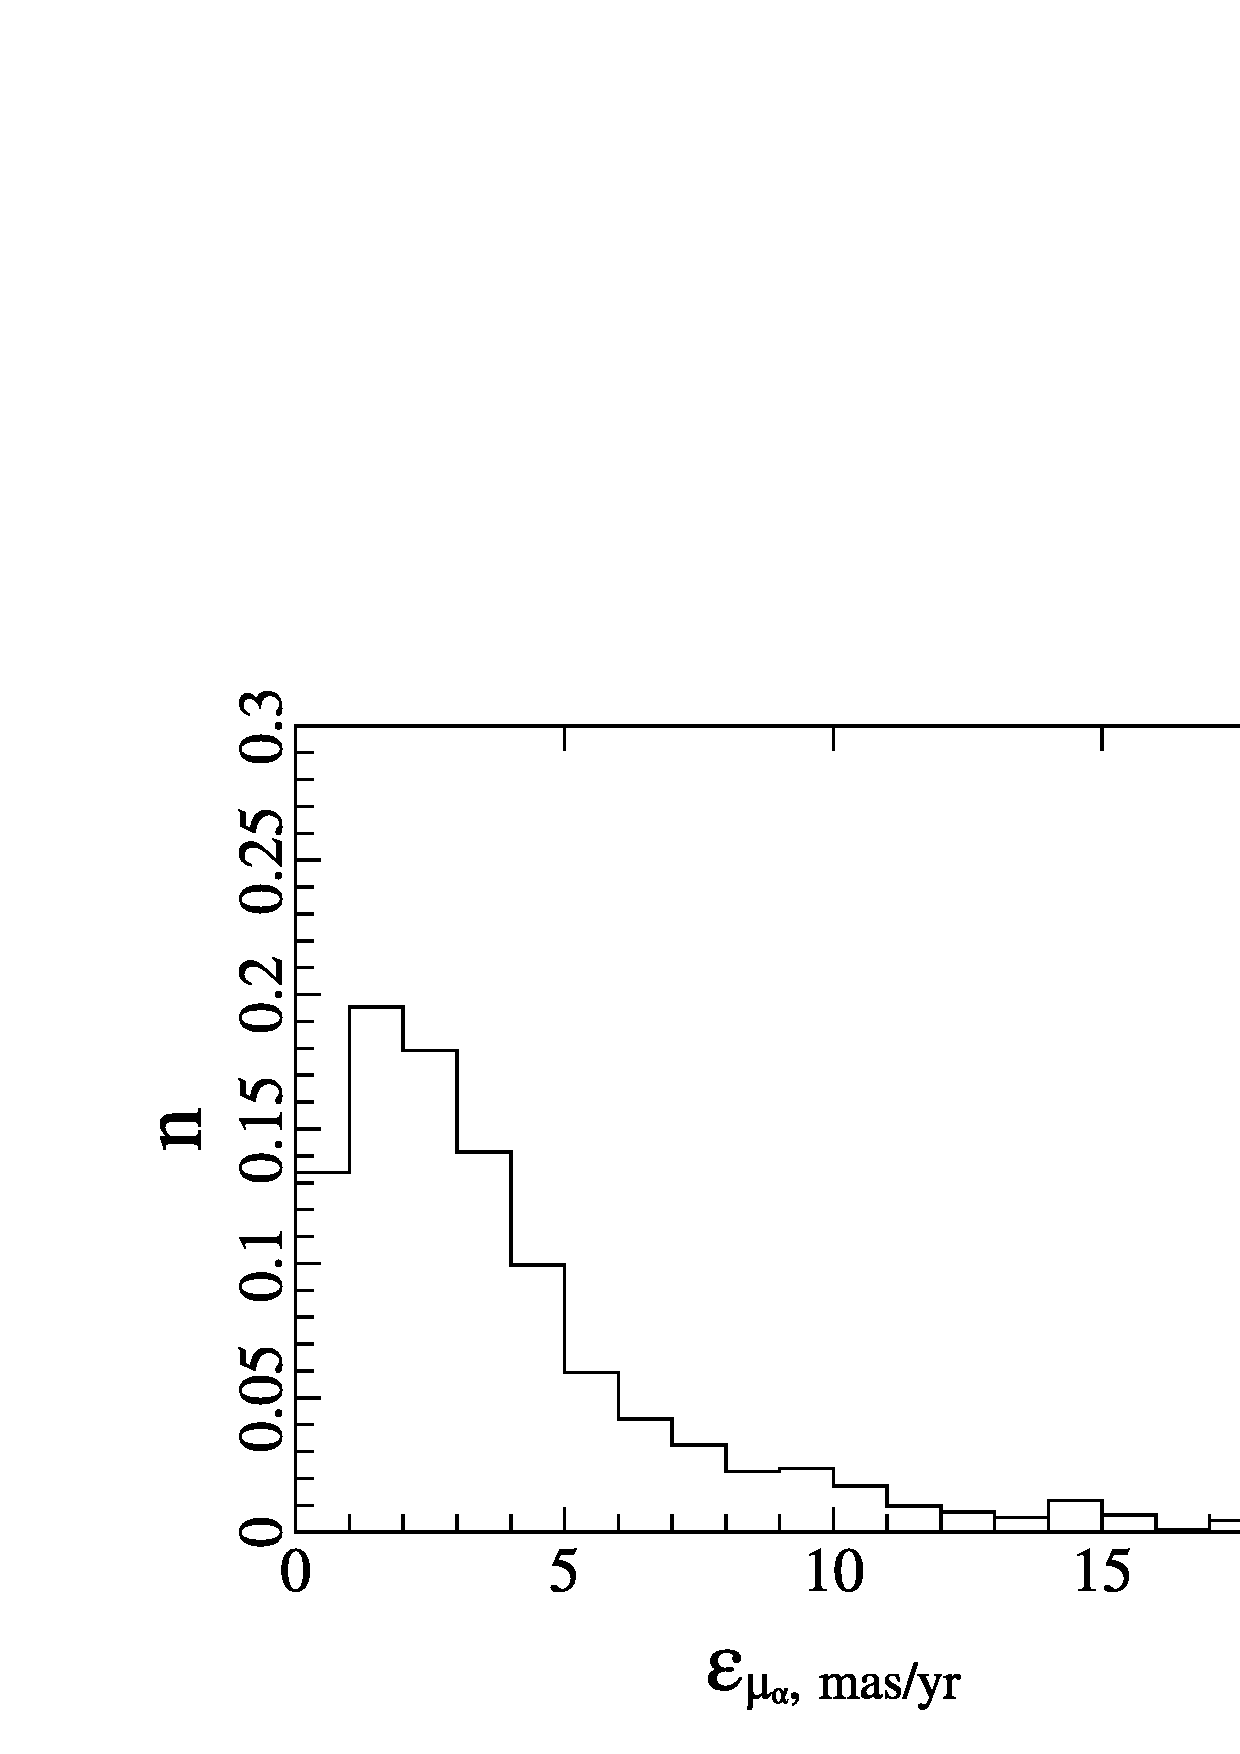
\includegraphics[width=1\columnwidth]{fig8a}
\column{0.5\textwidth}	
	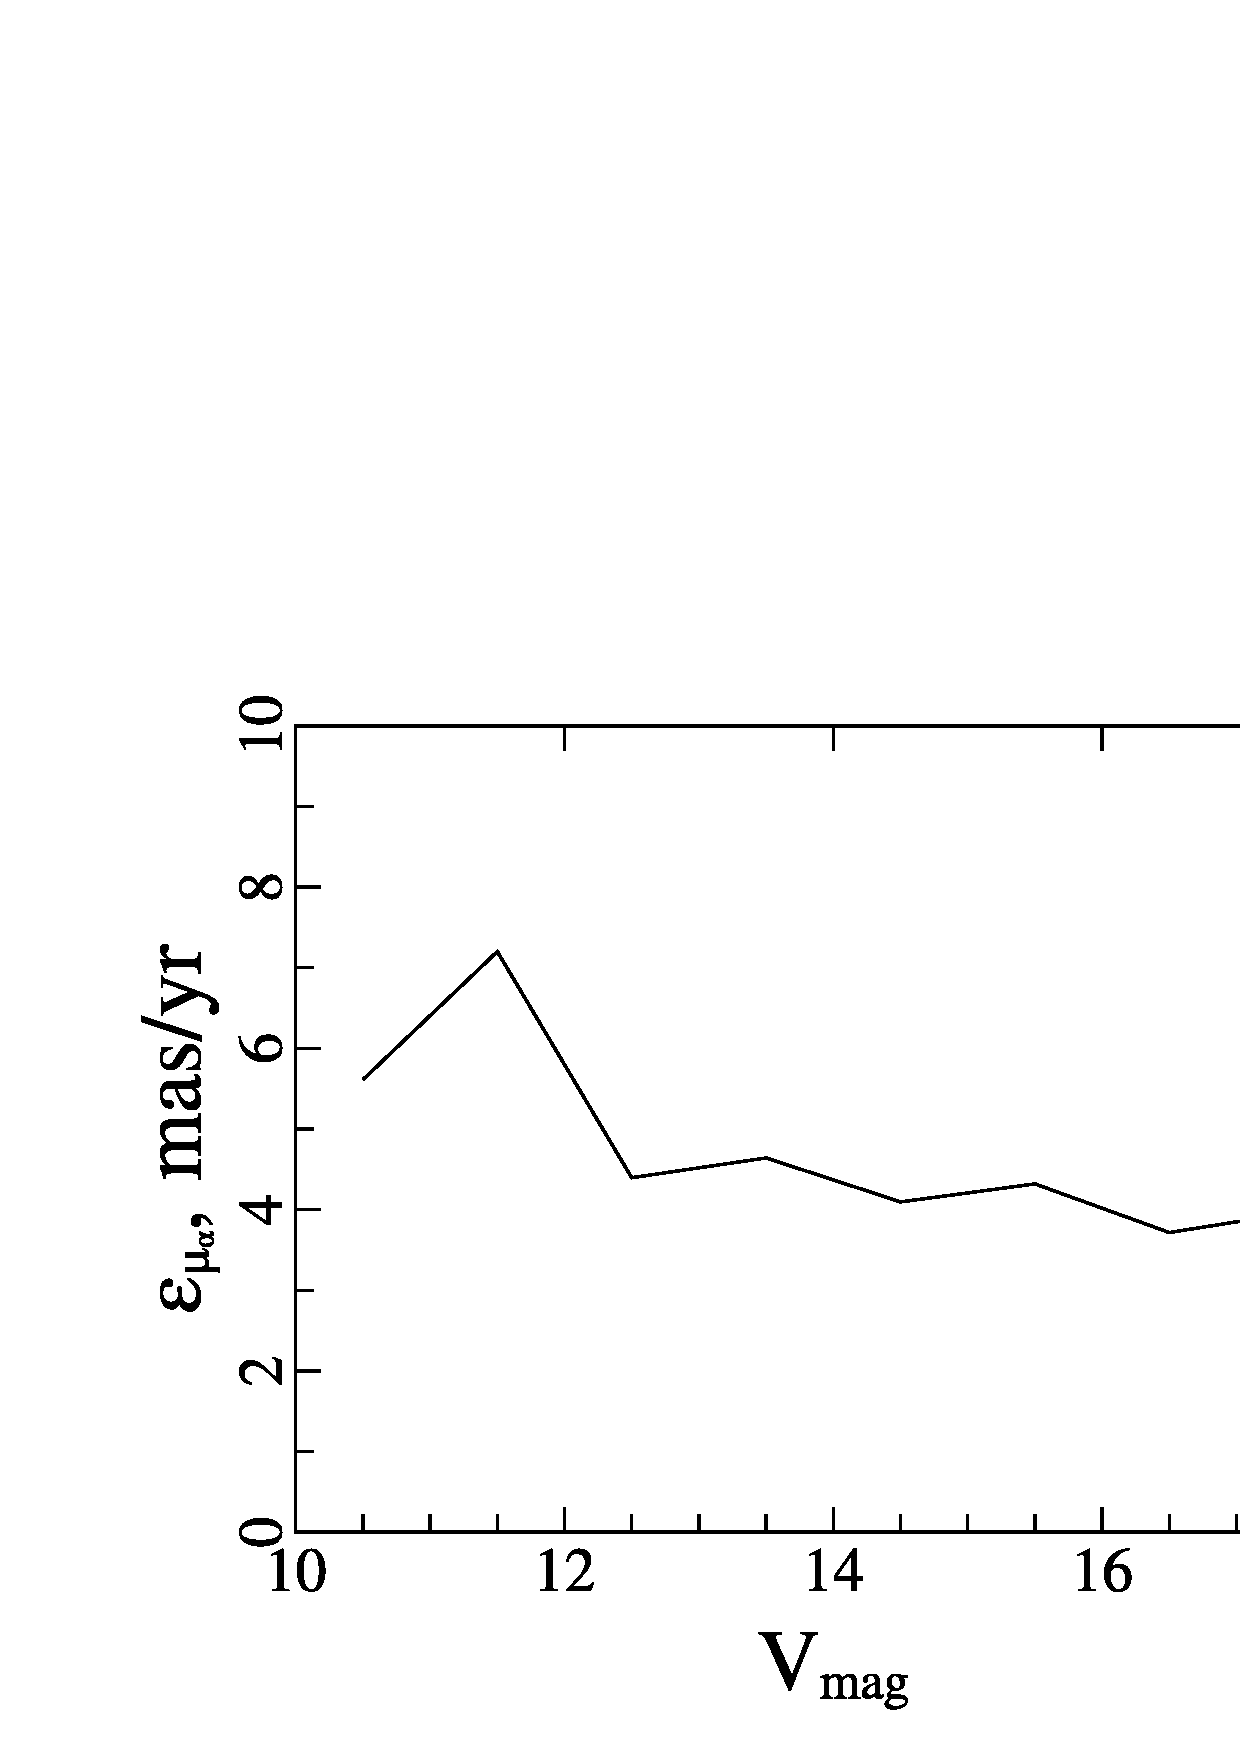
\includegraphics[width=1\columnwidth]{fig8b}
\end{columns}
\end{center}
{\footnotesize Распределение собственных ошибок собственных движений, построенных по всем точкам.}
\end{frame}


\begin{frame}%{{\tiny \it $\Delta\mu$-двойные среди близких карликов. Итоги}}
\frametitle{$\Delta\mu$-двойные среди близких карликов\\{\small собственные движения}}
\begin{center}
\begin{columns}
\column{0.5\textwidth}
	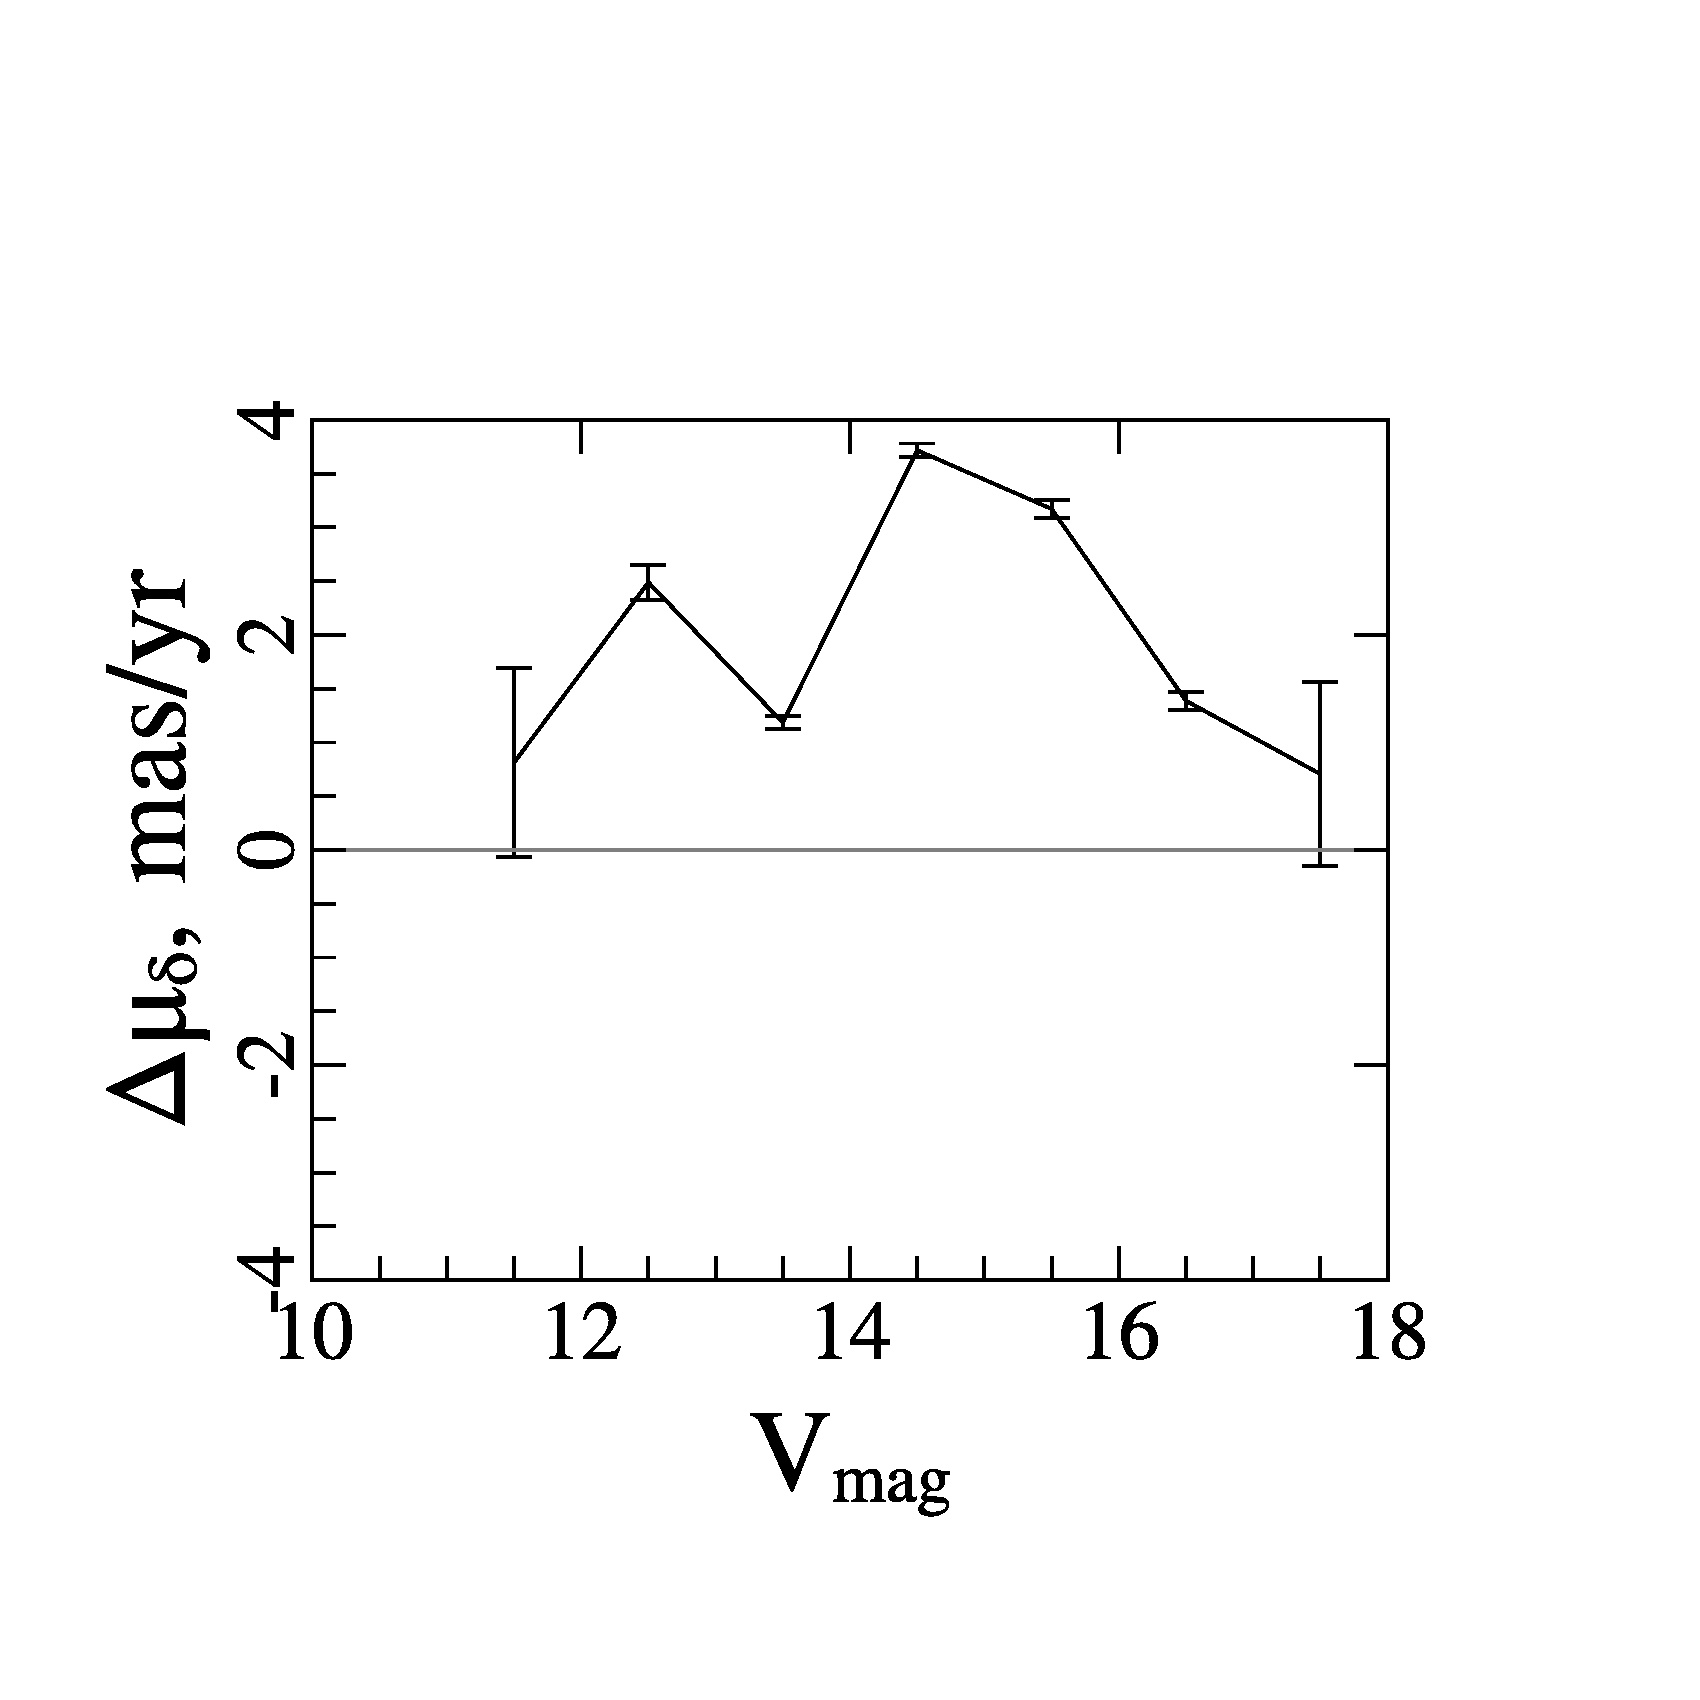
\includegraphics[width=1\columnwidth]{fig9a}
\column{0.5\textwidth}	
	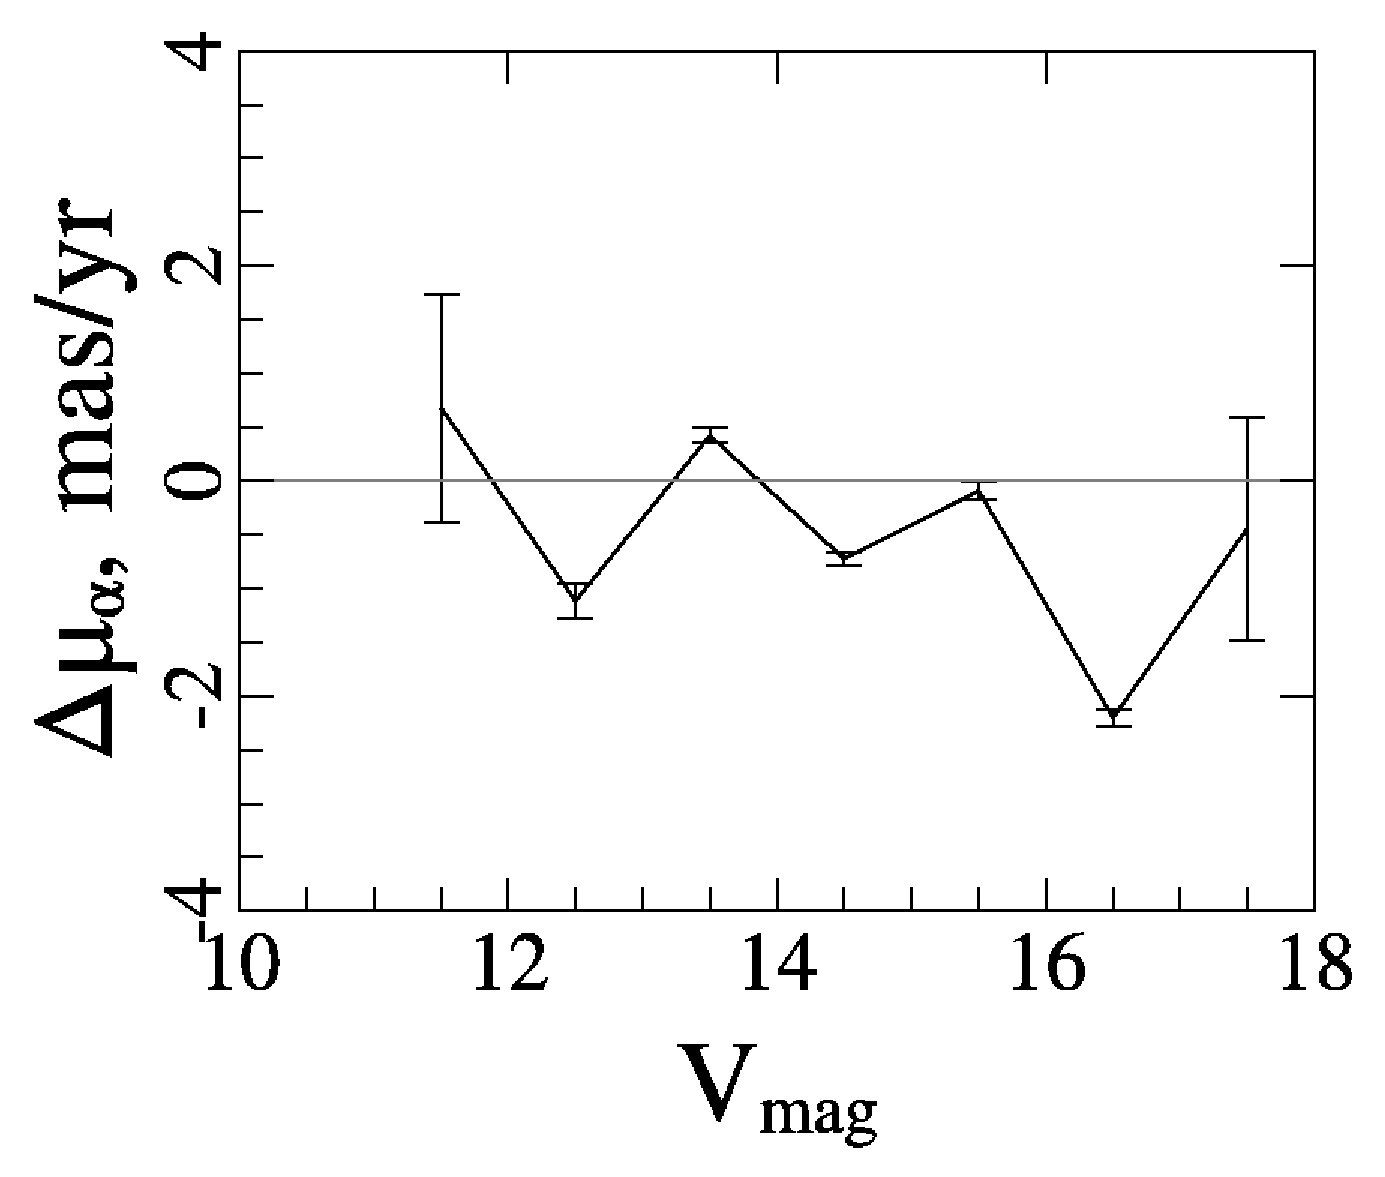
\includegraphics[width=1\columnwidth]{fig9b}
\end{columns}
\end{center}
{\footnotesize $\Delta \mu = \mu - \mu_{LSPM}$, $\mu$ --- по всем кадрам.}
\end{frame}


\begin{frame}
\frametitle{$\Delta\mu$-двойные среди близких карликов\\{\small параметр}}
\begin{center}
$F^2=\left(\frac{\Delta\mu_\alpha\cos\delta}{\varepsilon_{\mu_\alpha}}\right)^2 + \left(\frac{\Delta\mu_\delta}{\varepsilon_{\mu_\delta}}\right)^2$\\ \\
\end{center}
{\footnotesize
здесь $\Delta\mu = |\mu_{mean}-\mu_{inst}|$,  $\mu_{mean}$ --- [POSS2-POSS1], $\mu_{inst}$ --- все остальные точки; $\varepsilon_{\mu}$ "--- соответствующие взаимные стандартные ошибки.
}
\end{frame}

\begin{frame}%{{\tiny \it $\Delta\mu$-двойные среди близких карликов. Итоги}}
\frametitle{$\Delta\mu$-двойные среди близких карликов\\{\small пограничные значения параметра}}
\begin{center}
\begin{columns}
\column{0.5\textwidth}
	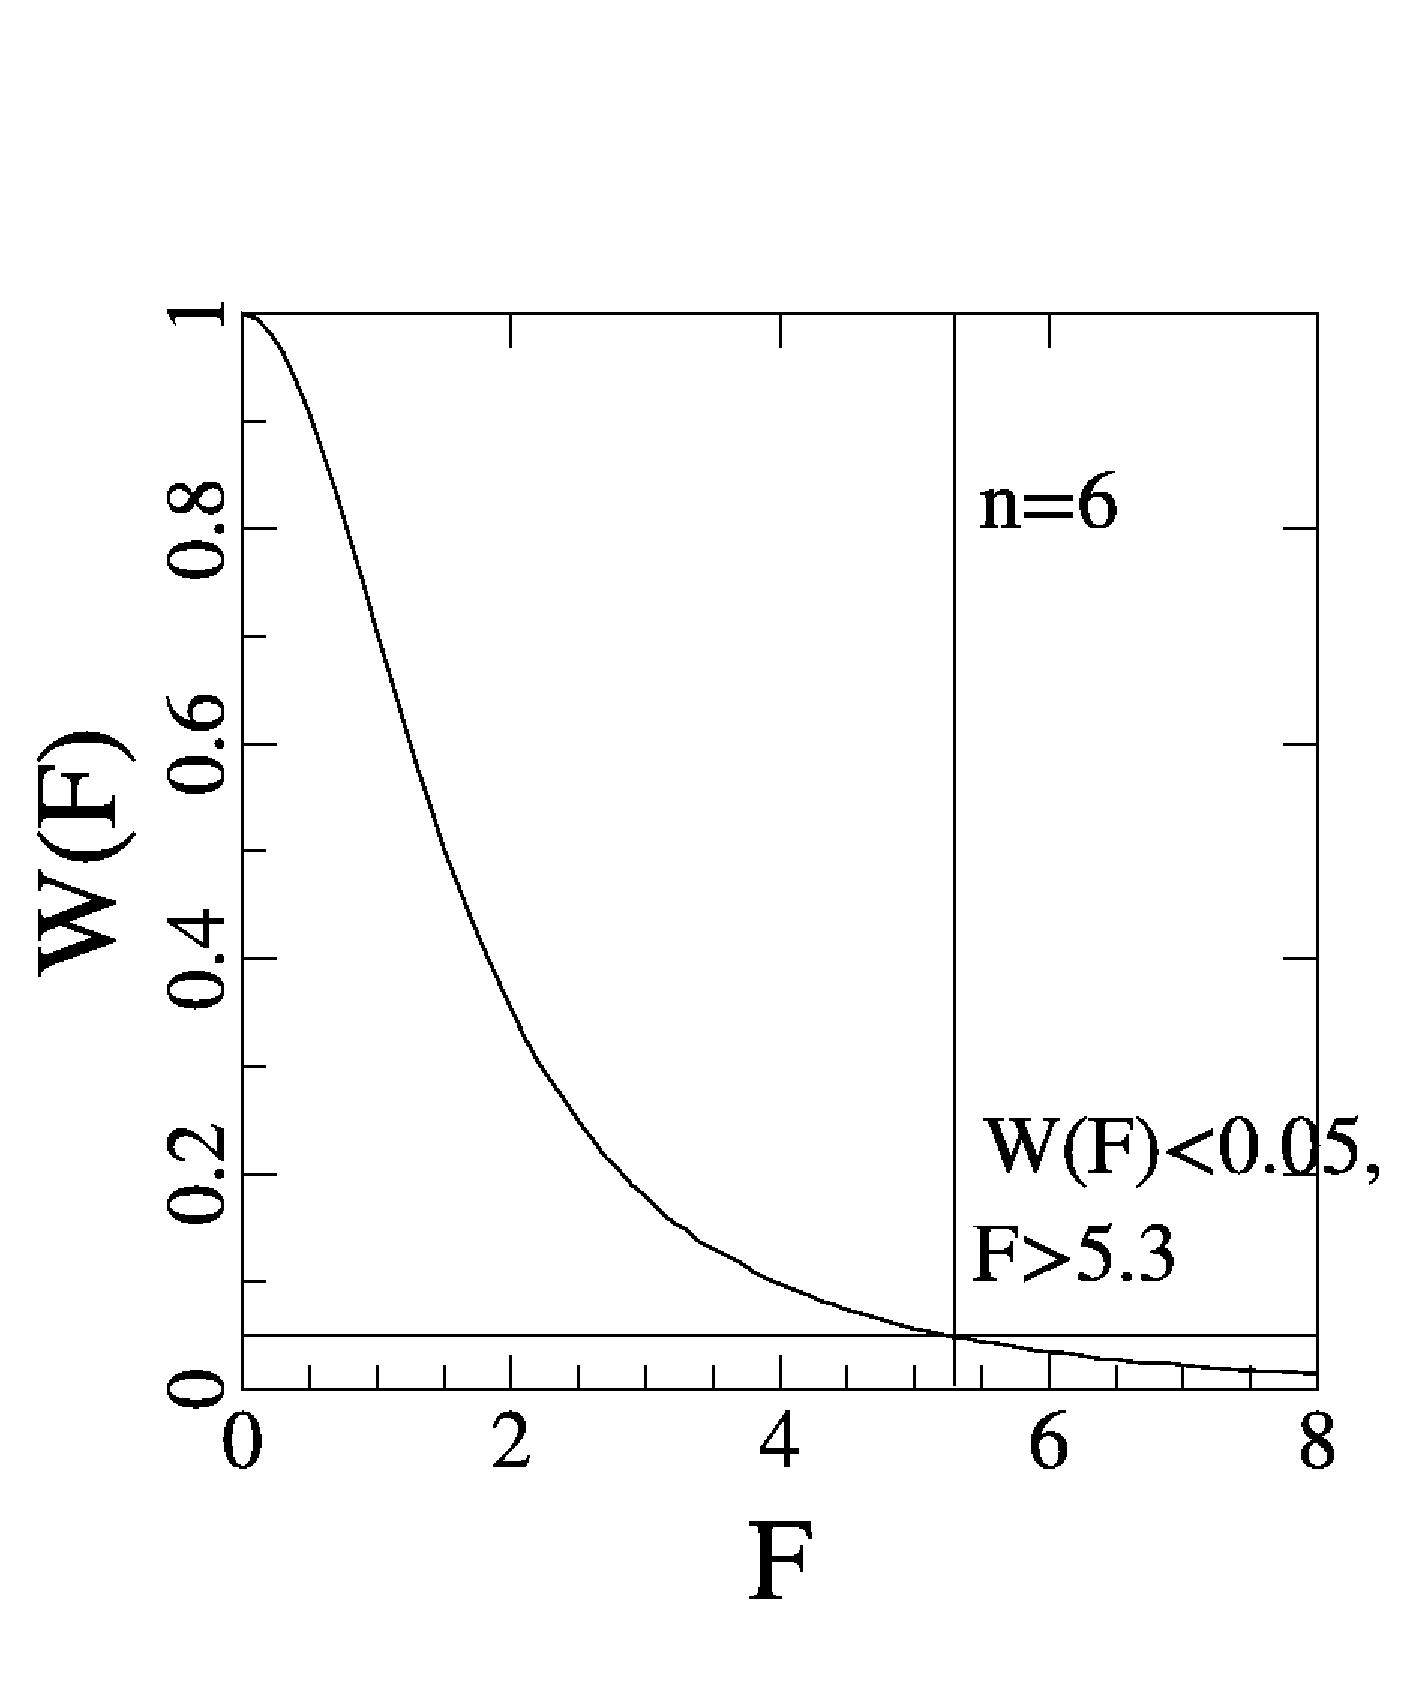
\includegraphics[width=0.8\columnwidth]{fig7a}
\column{0.5\textwidth}	
	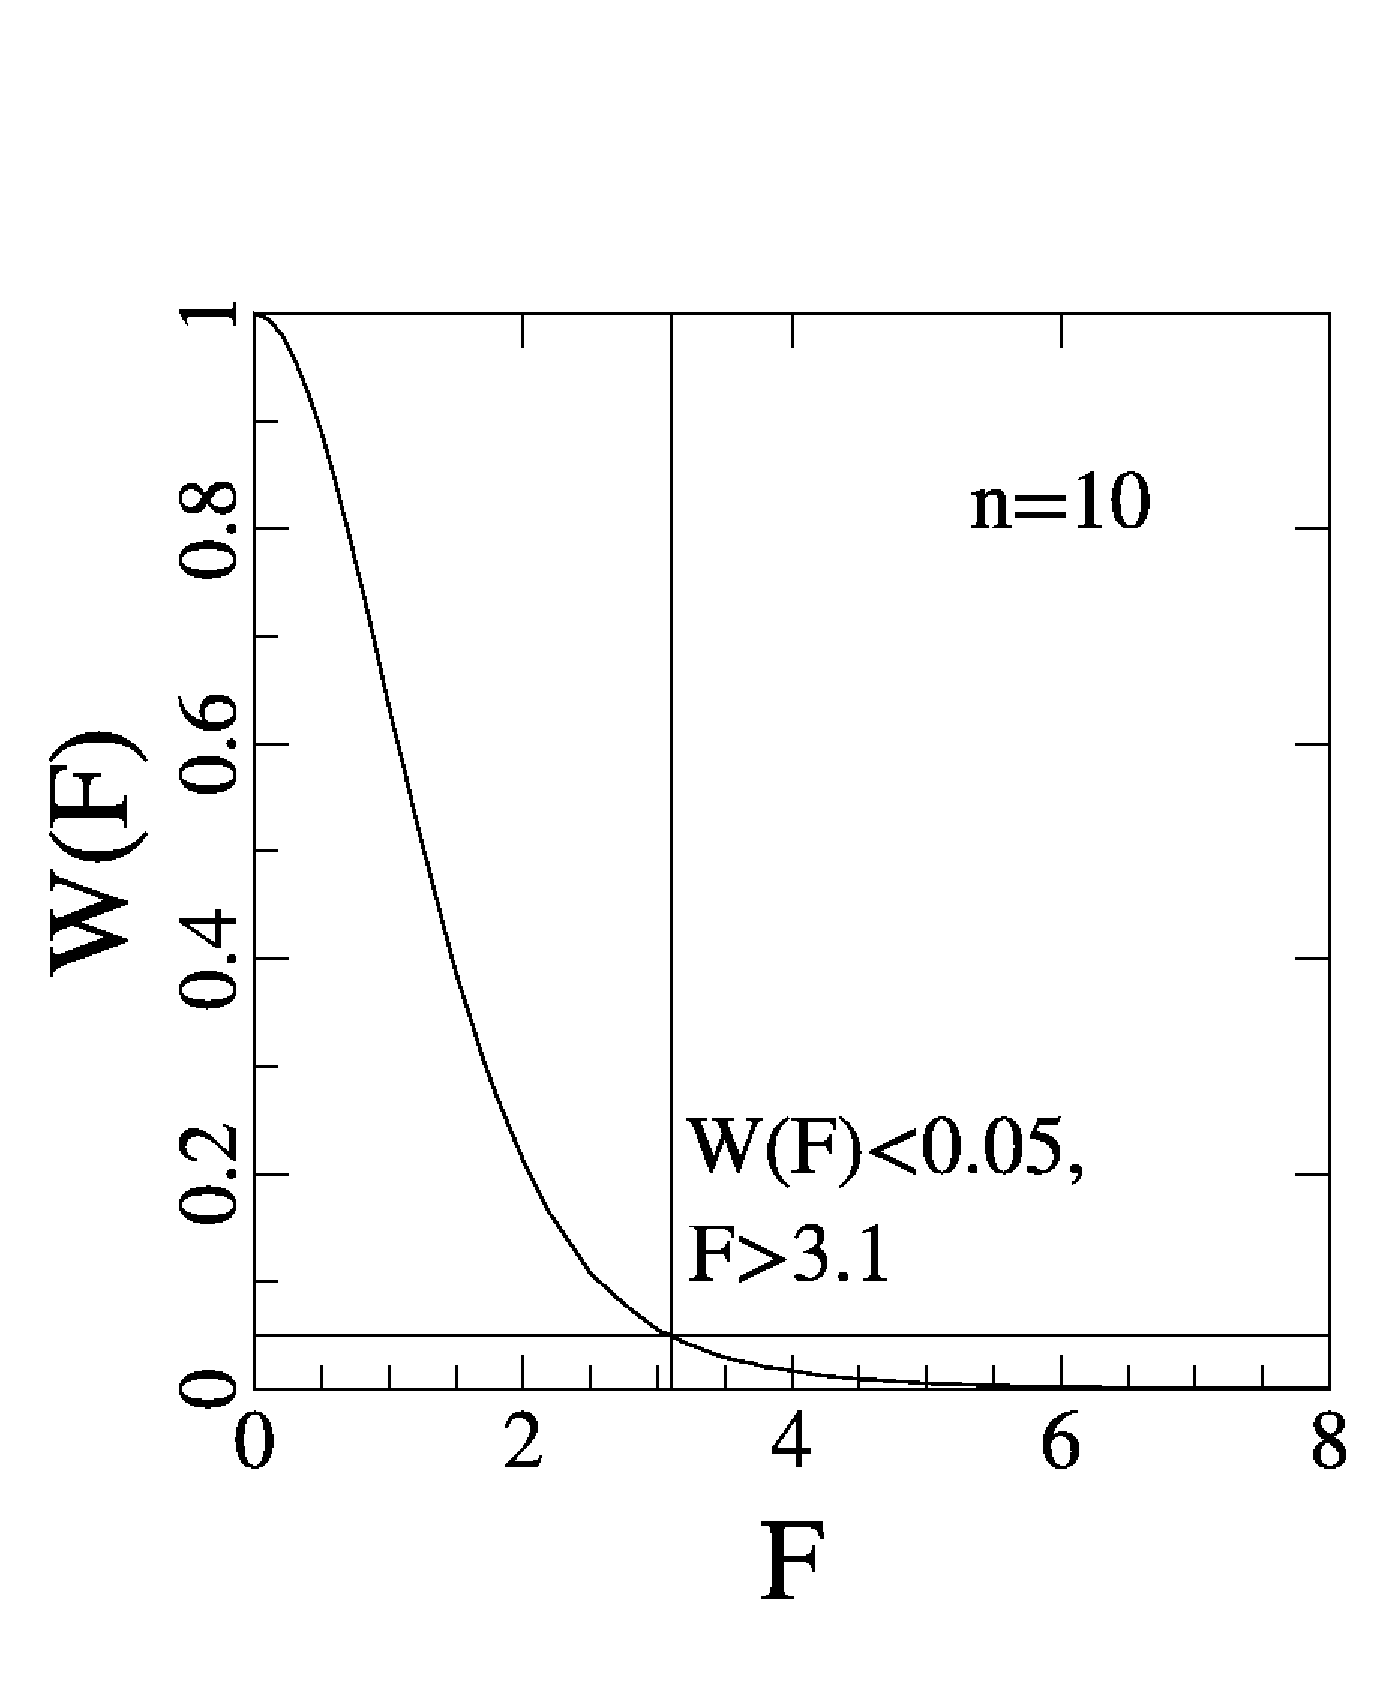
\includegraphics[width=0.8\columnwidth]{fig7b}
\end{columns}
\end{center}
{\footnotesize Моделирование одиночной звезды с заданными ошибками. Слева: $n=6$, справа: $n=10$.}
\end{frame}


\begin{frame}
\frametitle{$\Delta\mu$-двойные среди близких карликов\\{\small верификация}}
\begin{columns}
\column{0.5\textwidth}
	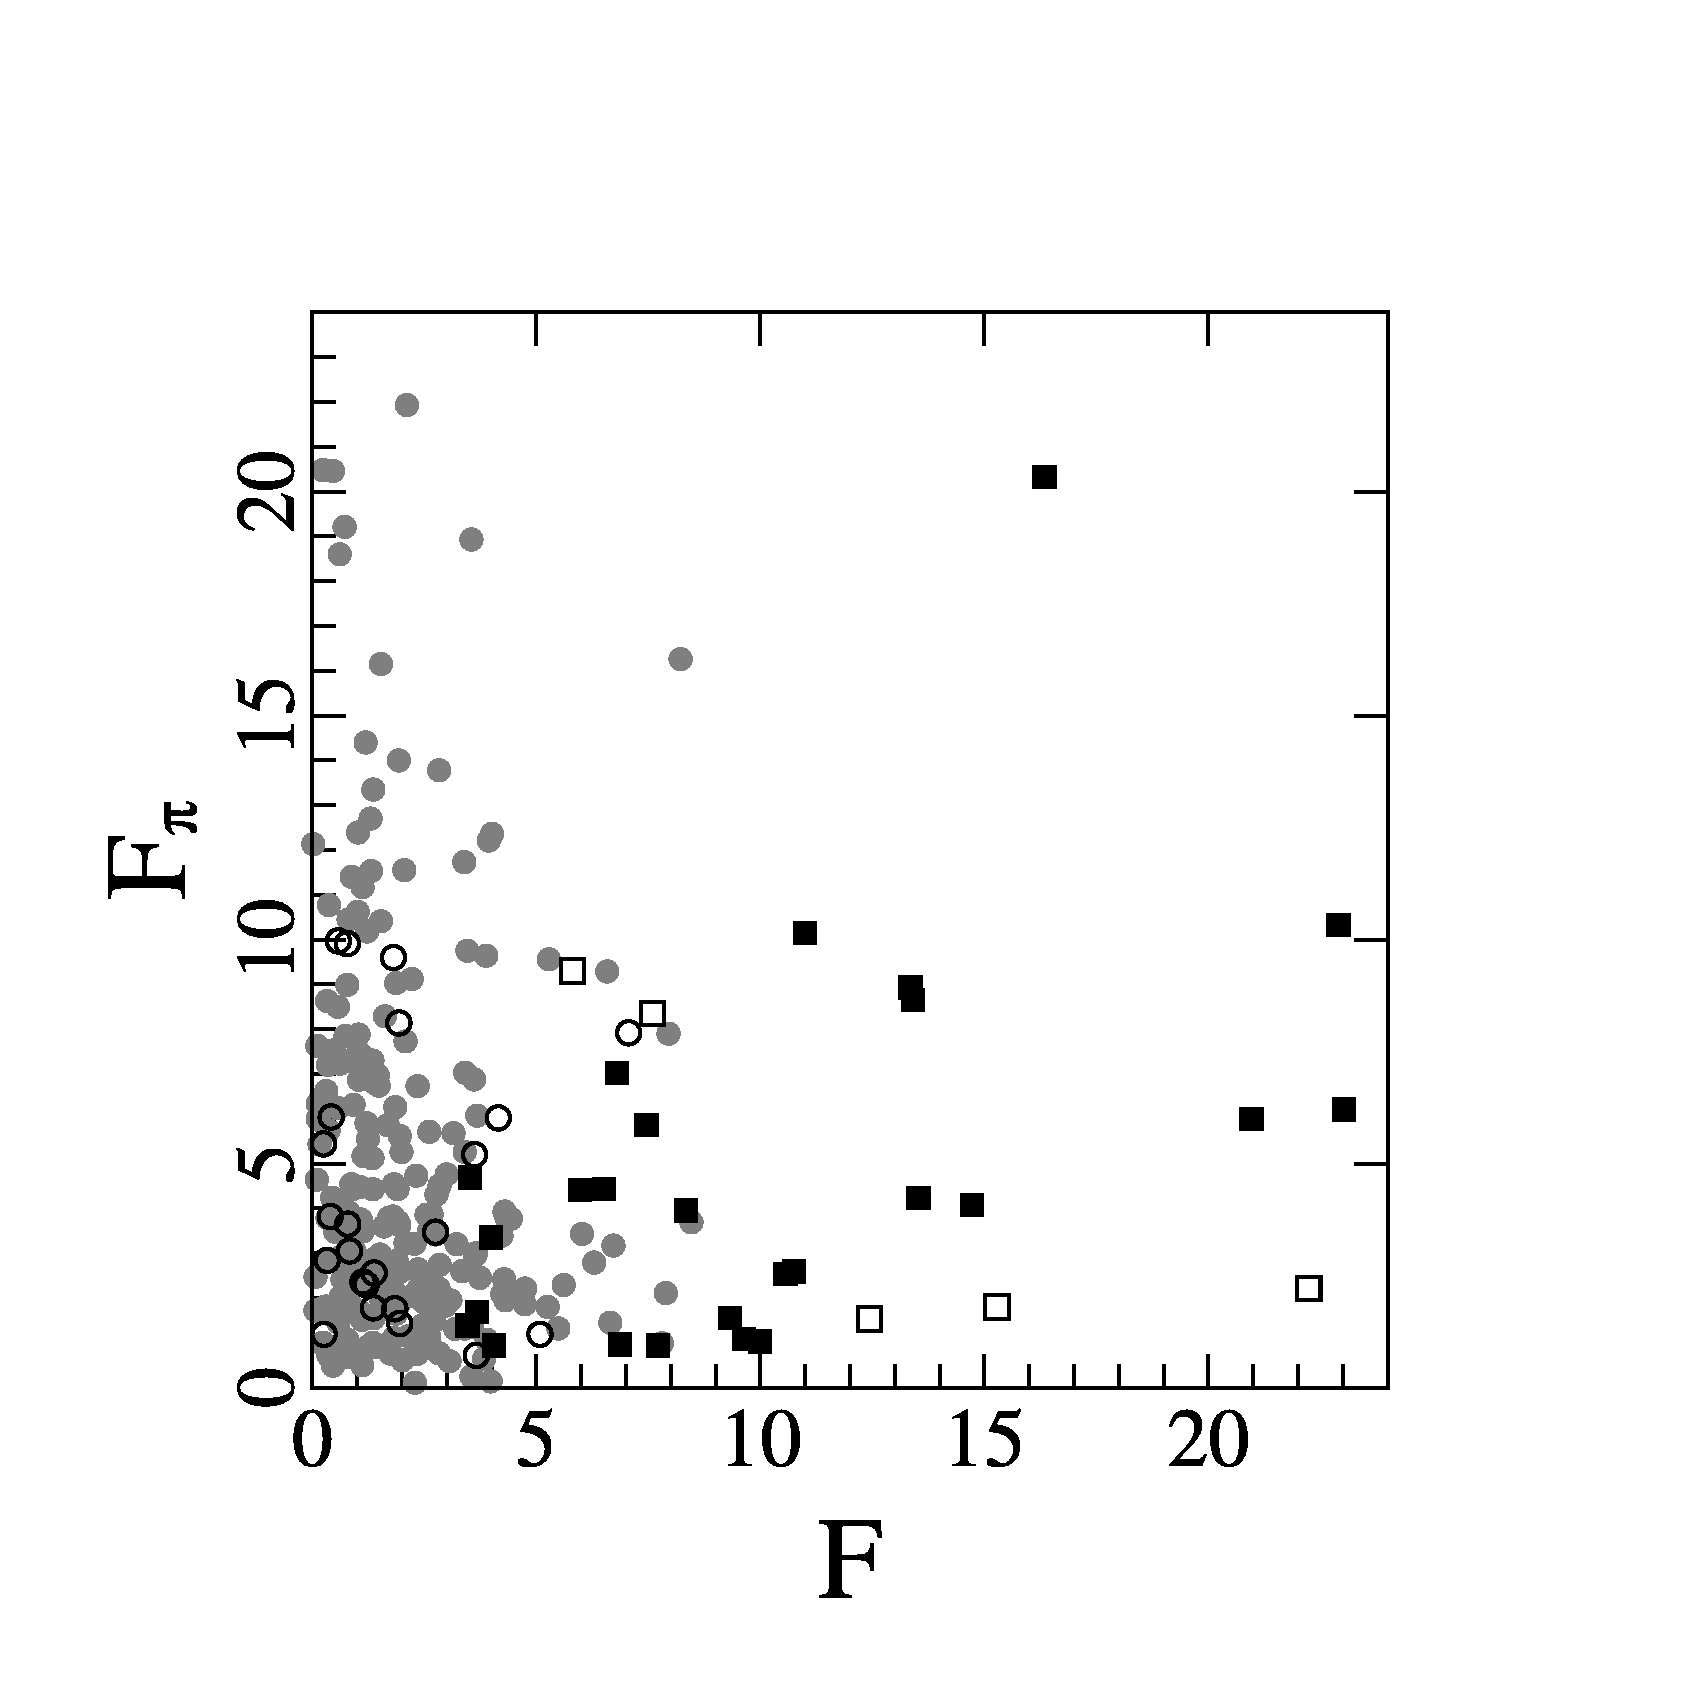
\includegraphics[width=1.1\columnwidth]{fig10}
\column{0.5\textwidth}	
	{\footnotesize
		$F_{\pi}$ --- по $\mu$, полученным из параллктических программ (3\,--\,5 лет). Кружки - <<одиночные>> звезды, квадраты - $\Delta\mu$-двойные. Присутствующие в WDS --- не закрашены. 
	}
\end{columns}
\end{frame}


\begin{frame}
\frametitle{$\Delta\mu$-двойные среди близких карликов\\{\small верификация}}
\begin{columns}
\column{0.5\textwidth}
	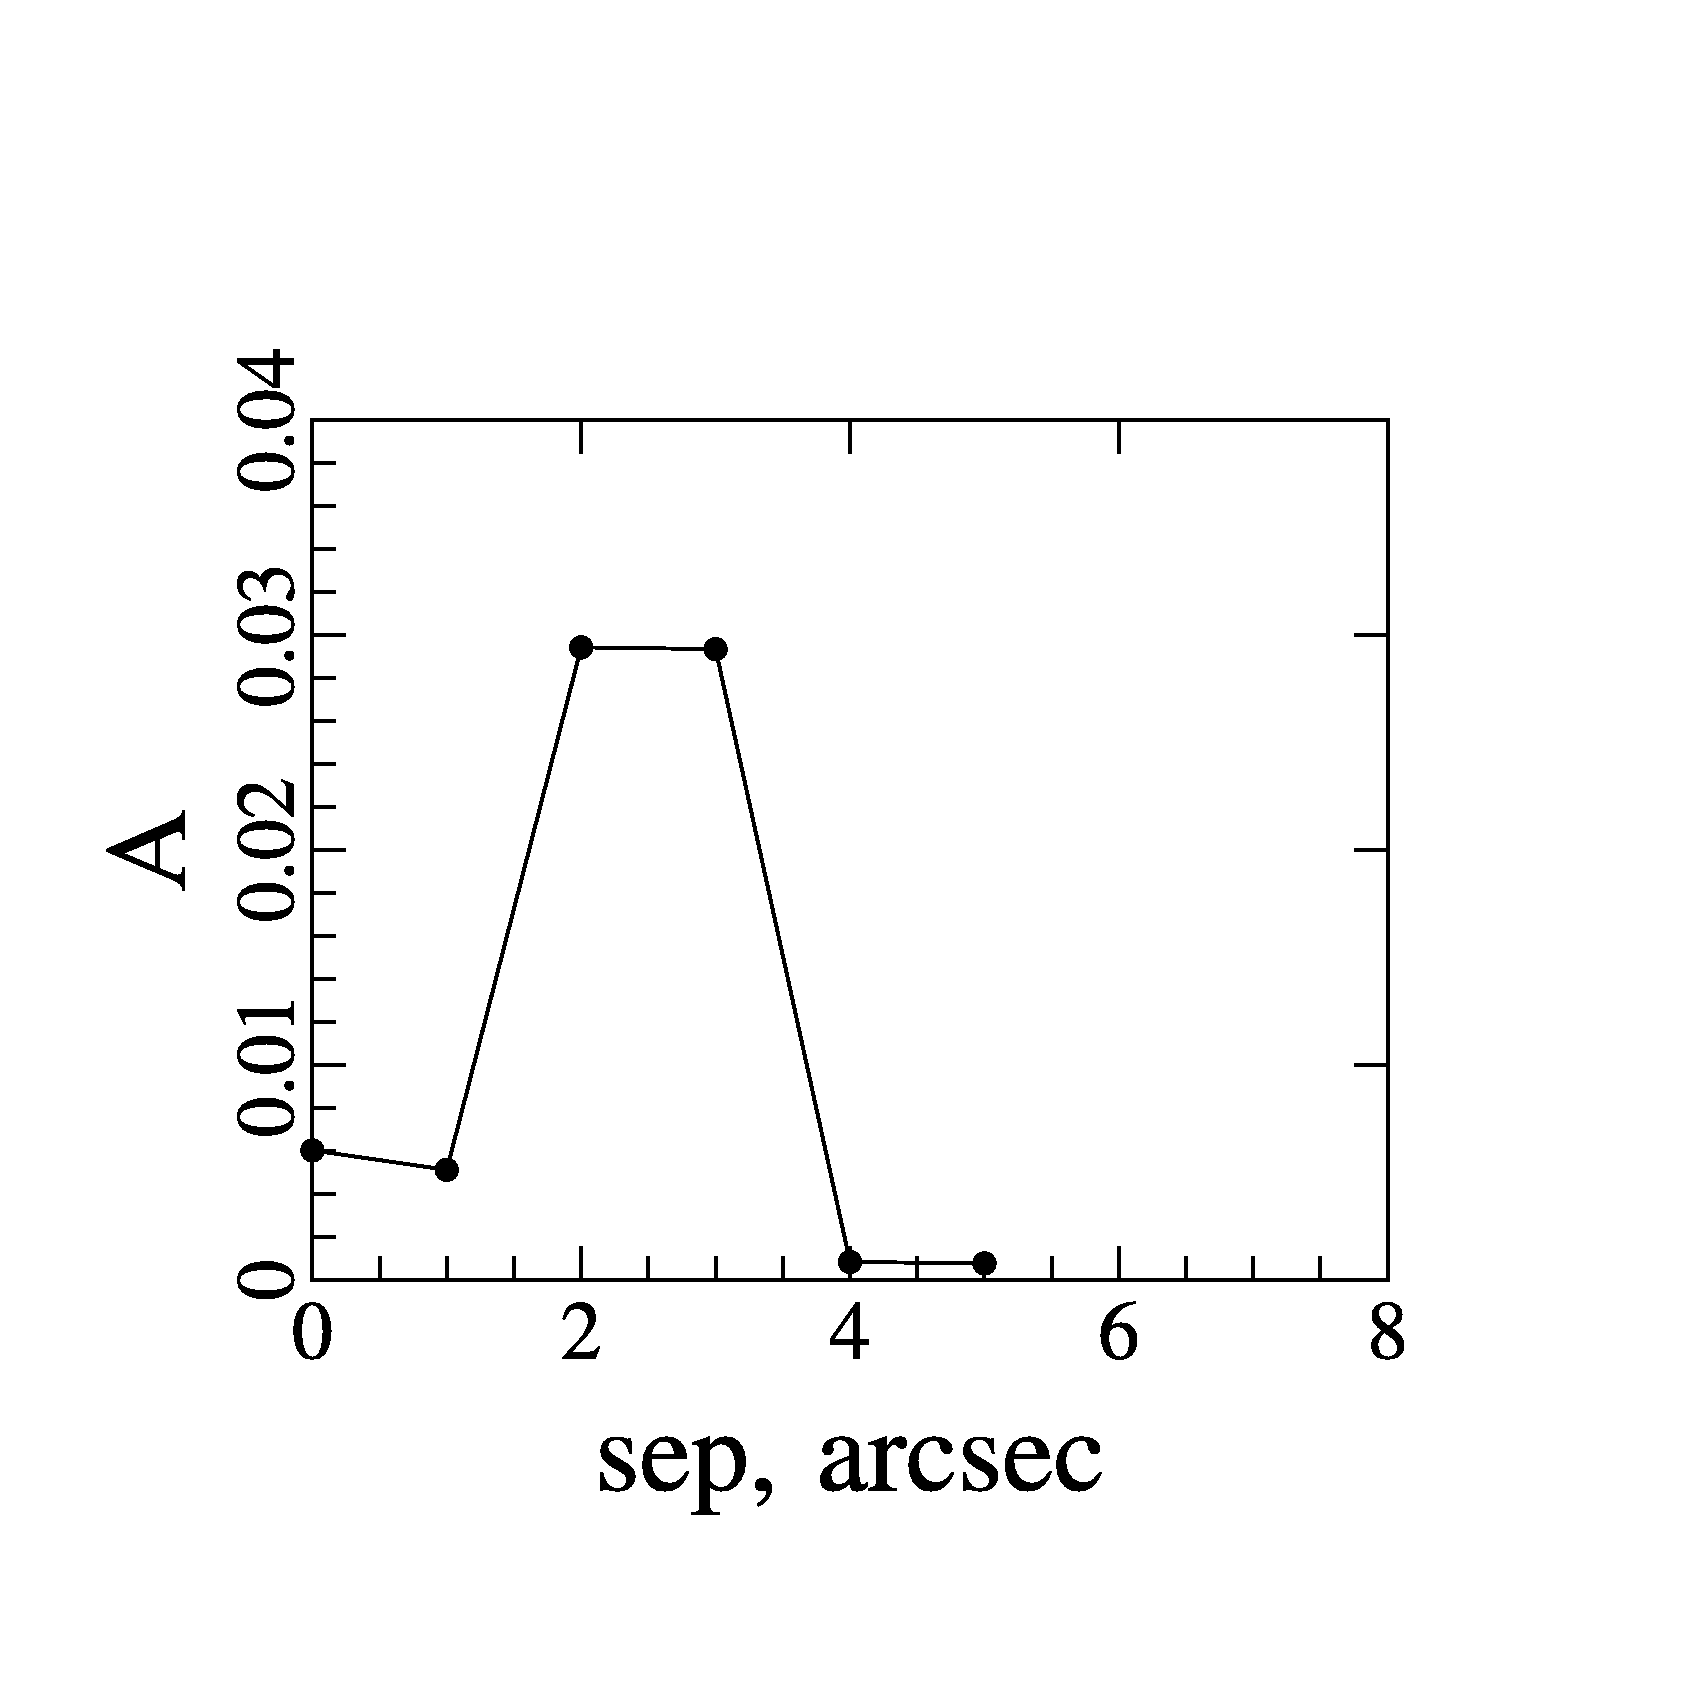
\includegraphics[width=1.1\columnwidth]{fig11}
\column{0.5\textwidth}	
	{\footnotesize
		Симуляция зависимости асимметрии взаимодействующих изображений от углового расстояния между компонентами ($14.1^m$, $15.3^m$) 
	}
\end{columns}
\end{frame}


\begin{frame}
\frametitle{$\Delta\mu$-двойные среди близких карликов\\{\small верификация}}
\begin{center}
\begin{columns}
\column{0.5\textwidth}
	\includegraphics[width=0.8\columnwidth]{fig12a}
\column{0.5\textwidth}	
	\includegraphics[width=0.8\columnwidth]{fig12b}
\end{columns}
\end{center}
{\footnotesize 
	Модель на основе падуанских изохрон и безансонской модели Галактики. Диапазон масс: $0.1\,M_{\odot}$~--~$0.7\,M_{\odot}$. Слева --- одиночные звезды. Справа - при добавлении пар <<M-карлик~+~белый~карлик>>. Массы белых карликов: $0.3\,M_{\odot}$ и $0.6\,M_{\odot}$, возраста: 0.6 и 1 Gyr соответственно.
}
\end{frame}


\begin{frame}
\frametitle{$\Delta\mu$-двойные среди близких карликов\\{\small результаты}}
%{\tiny 
\begin{itemize}
\item 121 звезда может рассматриваться как кандидат в $\Delta\mu$-двойные (\href{https://ui.adsabs.harvard.edu/abs/2015AstL...41..833K/abstract}{Khovrichev and Kulikova (2015)}).
\item 10 звезд из этого списка обнаружились в каталоге WDS (то есть это были уже известные двойные).
\item Список $\Delta\mu$-двойных доступен в \href{http://vizier.u-strasbg.fr/viz-bin/VizieR-3?-source=J/PAZh/41/896/lpmsm15b}{CDS}.
\end{itemize}
%}
\end{frame}



%%%%%%%%%%%%%%%%%%%%%%%%%%%%%%%%%%%%%%%%%%%%----------Эллиптичность и асимметрия----------------------------%%%%%%%%%%%%%%%%%%%%%%%%%%%%%%%%%%%%%%%%%%%%%%%%%%%%%%



\begin{frame}
\frametitle{Эллиптичность изображения}
\begin{center}
	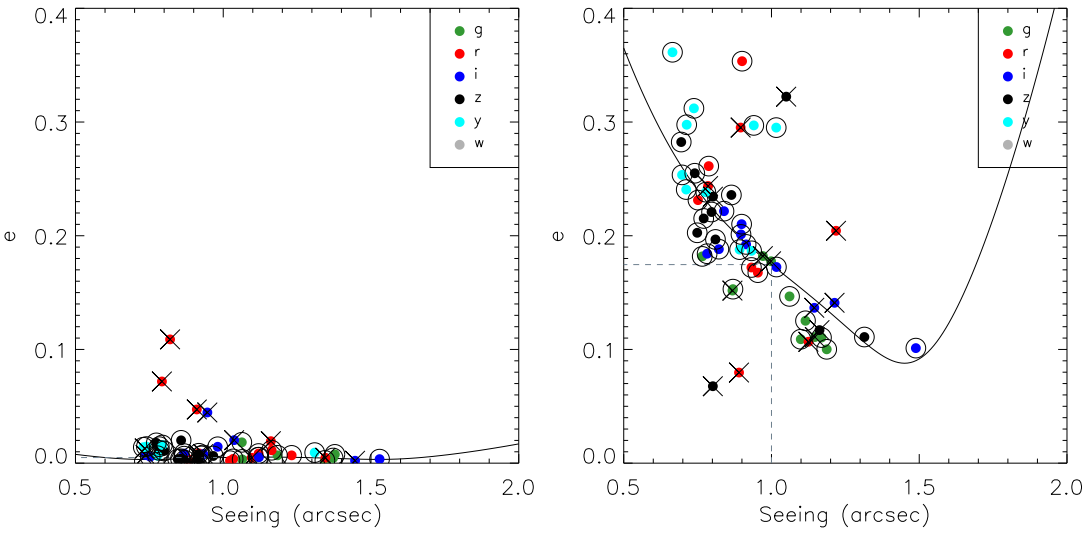
\includegraphics[width=0.8\textwidth]{Deacon-ellipticity}
\end{center}
{\footnotesize
	Deacon et al., 2017
}
\end{frame}


\begin{frame}
\frametitle{Эллиптичность изображения}
%{\footnotesize
	Моменты распределения интенсивности:\\[5pt]
	$q_{xx}=\sum x^2 I(x,y)$,\\ $q_{xy}=\sum xy I(x,y)$,\\ $q_{yy}=\sum y^2 I(x,y)$,\\[10pt]
	$I(x,y)$ - изображение звезды.\\[15pt]
	Эллиптичность изображения:\\[5pt]
	$e_1 = \frac{q_{xx}-q_{yy}}{q_{xx}+q_{yy}}$,\qquad $e_2 = \frac{q_{xy}}{q_{xx}+q_{yy}}$,\qquad $e^2=e^2_1+e^2_2$
%}
\end{frame}


\begin{frame}
\frametitle{Эллиптичность и асимметрия}
\begin{center}
{\small
\begin{align*}
\left[e_1,~e_2\right] = \left[\frac{q_{xx}-q_{yy}}{q_{xx}+q_{yy}},~\frac{q_{xy}}{q_{xx}+q_{yy}}\right],\: e = \sqrt{e_1^2+e_2^2}\\[15pt]
A = F^{-1}\cdot \sum_{pixels} |I(x,y)-I(x,y)^{180}|
\end{align*}
}
\end{center}
{\footnotesize
	Эллиптичность вычисляется через квадрупольные моменты, индекс асимметрии --- через поворот исходного изображения $I(x,y)$ на $180^\circ$.
}
\end{frame}


\begin{frame}
\frametitle{Эллиптичность и асимметрия}
\begin{center}
\begin{columns}
\column{0.5\textwidth}
	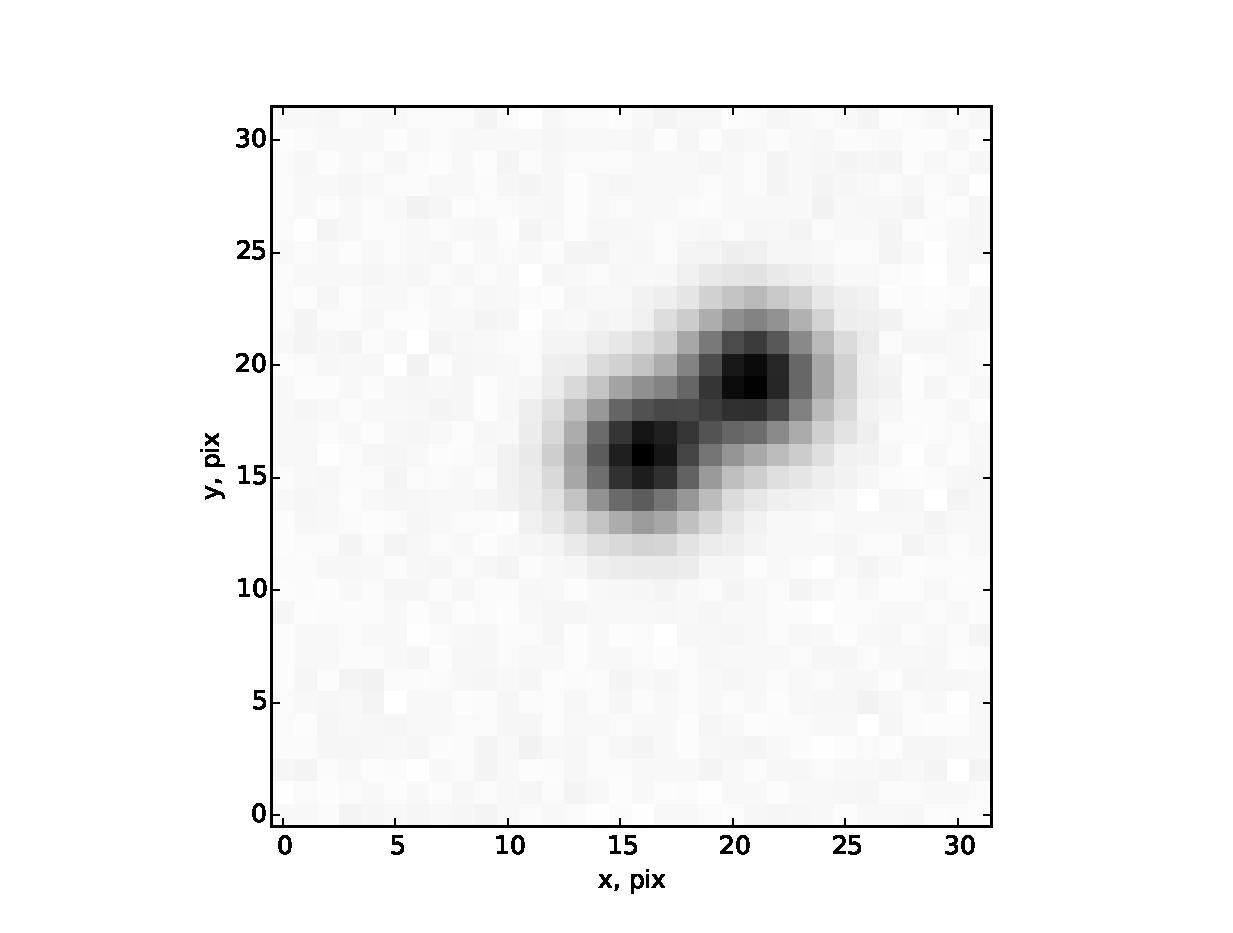
\includegraphics[width=0.8\columnwidth]{asy_6_35_00_100_008_0410}
\column{0.5\textwidth}	
	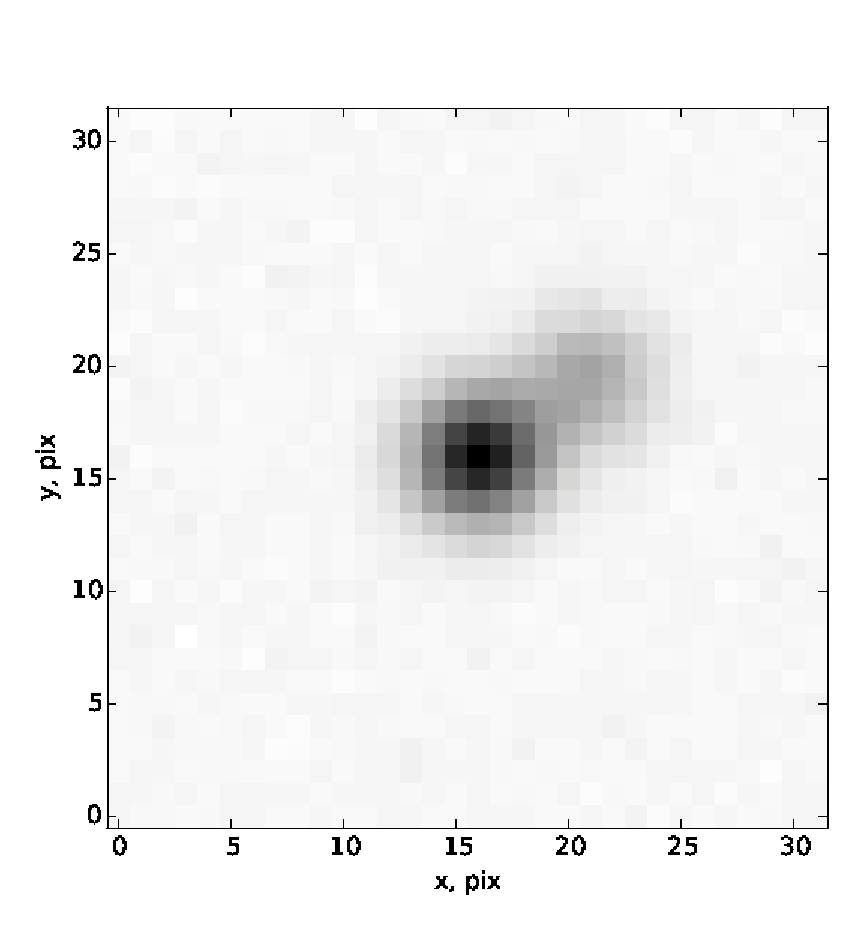
\includegraphics[width=0.8\columnwidth]{asy_6_35_10_100_071_035}
\end{columns}
\end{center}
{\footnotesize 
	Модельные изображения.\\ Слева: $\rho = 6\,pix$, $\Theta = 55^{\circ}$, $\Delta m = 0^m$, $e_t = 0.41$, $A_t = 0.08$.\\ Справа:  $\rho = 6\,pix$, $\Theta = 55^{\circ}$, $\Delta m = 1^m$, $e_t = 0.35$, $A_t = 0.71$.
}
\end{frame}


\begin{frame}
\frametitle{Эллиптичность и асимметрия}
\begin{center}
{\small
\begin{align*}
	S_e=(e_t-e_b)/\sigma_e, \qquad S_A=(A_t-A_b)/\sigma_A\\[10pt]
	\sigma_e^2=\epsilon_{e_b}^2+\epsilon_{e_t}^2, \qquad \sigma_A^2=\epsilon_{A_b}^2+\epsilon_{A_t}^2
\end{align*}
}
\end{center}
{\footnotesize
	К двойным относились звезды, для которых $S_e \geqslant 3$ и/или $S_A \geqslant 3$ 
}
\end{frame}


\begin{frame}
\frametitle{Эллиптичность и асимметрия\\{\small формирование списка}}
\begin{center}
	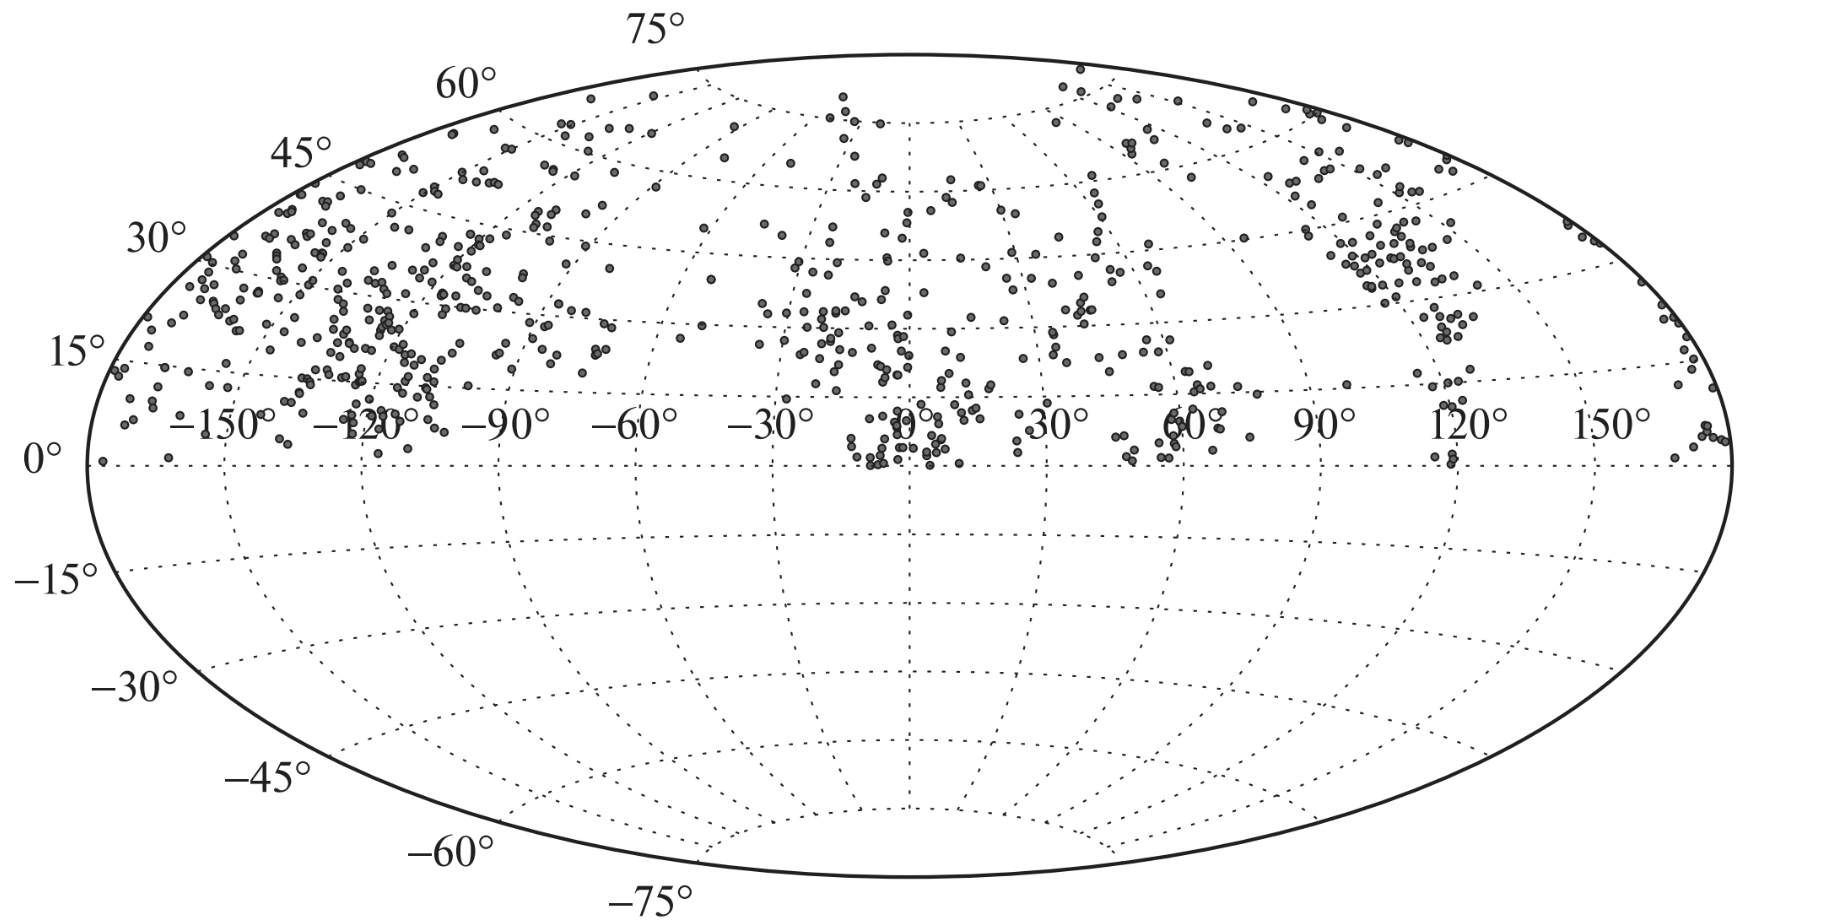
\includegraphics[width=0.8\textwidth]{khovr2018-6}
\end{center}
{\scriptsize
	702 звезды с флагом <<duplicate source>> (Gaia DR1) = 1. $V>13^m$, $\mu>300''/yr$. Наблюдения на телескопе <<Сатурн>>(Khovritchev et al., 2015) и материалы SDSS DR13 (Albareti et al., 2017).
}
\end{frame}


\begin{frame}
\frametitle{Эллиптичность и асимметрия\\{\small пример реальной звезды}}
\begin{center}
\begin{columns}
\column{0.5\textwidth}
	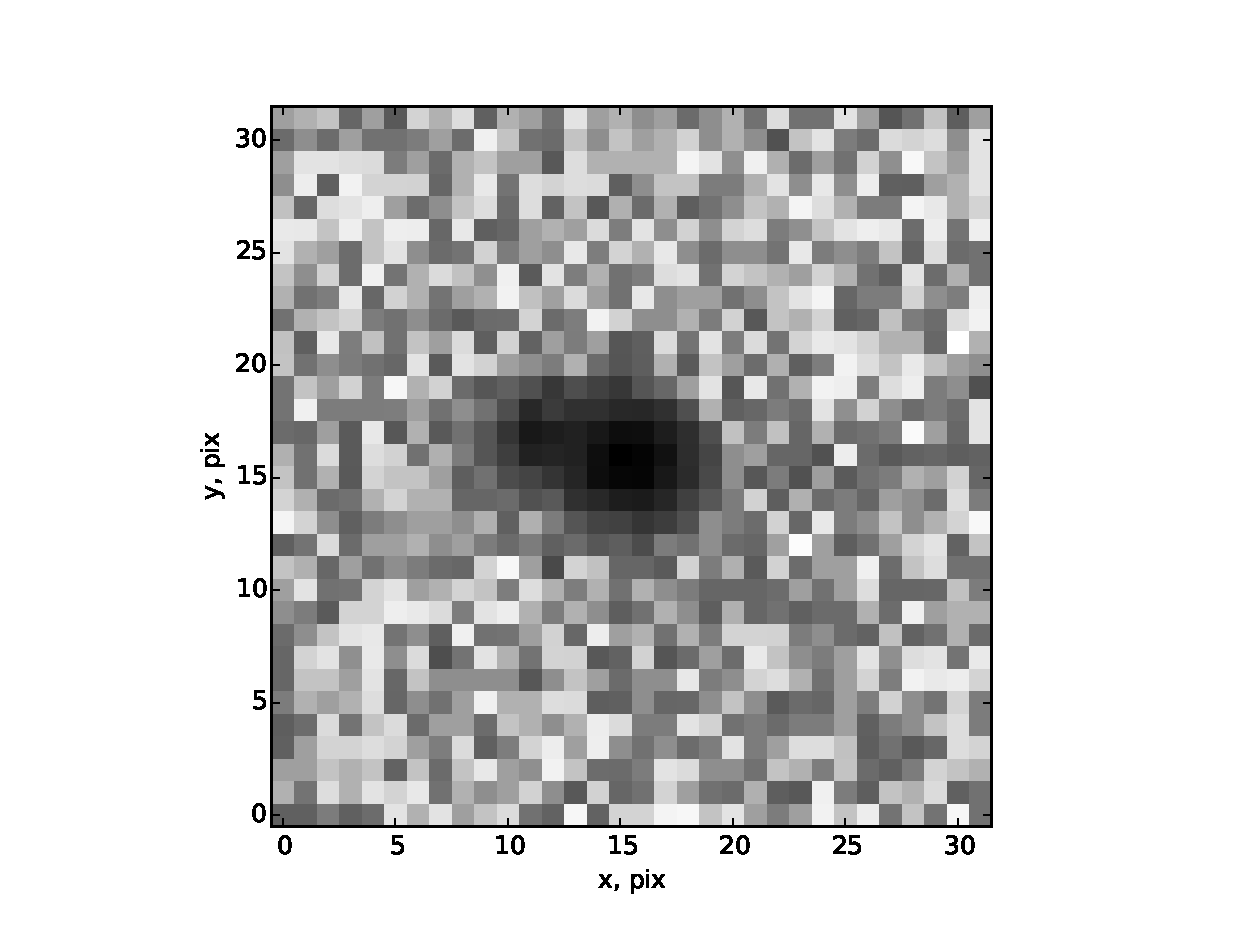
\includegraphics[width=0.7\columnwidth]{J0740+1706}
\column{0.5\textwidth}	
	\includegraphics[width=0.7\columnwidth]{J0740+1706-kernel}
\end{columns}
\end{center}
{\scriptsize 
	Слева: изображение звезды J0740+1706. Справа: PSF, построенная на основе медианных значений шейплет-коэффициентов звезд фона и оценки шума изображения. $e_{t} =0.349\pm0.031$,  $A_{t} = 0.597\pm0.035$. PSF: $e_{b} =0.084\pm0.060$,   $A_{b} =0.122\pm0.032$. $S_e=3.9$, $S_A=10.0$.
}
\end{frame}


\begin{frame}
\frametitle{Эллиптичность и асимметрия\\{\small результаты}}
\begin{itemize}
\item 144 звезды из 702 исследованных (<<duplicate source>>) на изображениях SDSS содержали значительные величины эллиптичности и/или асимметрии,
\item для 9 из 144 нашлись признаки двойственности и на кадрах <<Сатурна>> (разница эпох наблюдений $\approx$ 10 лет),
\item 6 из 144 оказались в WDS,
\item Список $\Delta\mu$-двойных доступен в \href{http://vizier.u-strasbg.fr/viz-bin/VizieR?-source=J/PAZh/44/124}{CDS}.
\end{itemize}
\end{frame}

\begin{frame}
\frametitle{Эллиптичность и асимметрия\\{\small верификация}}
\begin{center}
\begin{columns}
\column{0.5\textwidth}
	\includegraphics[width=0.8\columnwidth]{cmd}
\column{0.5\textwidth}	
	\includegraphics[width=0.8\columnwidth]{cmd-asy}
\end{columns}
\end{center}
{\footnotesize 
	Для 41 исследованного объекта есть $\pi_{trg}$, что позволило нанести их на диаграмму <<цвет -- абсолютная зв. величина>>.\\ Слева: системы, детектированные по обоим признакам.\\ Справа: системы со значительной асимметрией.
}
\end{frame}


%%%%%%%%%%%%%%%%%%%%%%%%%%%%%%%%%%%%%%%%%%%%----------Спекл----------------------------%%%%%%%%%%%%%%%%%%%%%%%%%%%%%%%%%%%%%%%%%%%%%%%%%%%%%%



\begin{frame}
\frametitle{Движение фотоцентра J1158+4239.}
\begin{columns}
\column{0.6\textwidth}
	\begin{center}
	\includegraphics[width=1.1\columnwidth]{16fig2}
	\end{center}
\column{0.4\textwidth}
	{\scriptsize 
		\begin{itemize}
		\item[] 1955 --- POSS1
		\item[] 1984 --- GSC1
		\item[] 1990 и 1991 --- POSS2
		\item[] 1996 --- GSC2
		\item[] 2003 --- SDSS
		\item[] 2012 - PNA
		\end{itemize}
		%1955 --- POSS1,\\[10pt] 1984 --- GSC1,\\[10pt] 1990 и 1991 --- POSS2,\\[10pt] 1996 --- GSC2,\\[10pt] 2003 --- SDSS,\\[10pt] 2012 - PNA. 
	}
\end{columns}
\begin{center}
{\scriptsize $\mu_{all}(\alpha)=-326.4\pm 1.7$~mas/yr, $\mu_{all}(\delta)=50.1\pm 7.1$~mas/yr, $\mu_{mean}(\alpha)=-336.9\pm 6.4$~mas/yr, $\mu_{mean}(\delta)=84.7\pm 6.3$~mas/yr, $\mu_{inst}(\alpha)=-303.7\pm 8.5$~mas/yr, $\mu_{inst}(\delta)=21.1\pm 7.9$~mas/yr,\\ F = 6.99.}
\end{center}
\end{frame}

\begin{frame}
\frametitle{Спекл-интерферометрия}
\begin{itemize}
\item[] БТА САО РАН:
\item[] $d=6$~м., EMCCD-камера Andor iXon Ultra
\item[] 
\item[] КГО ГАИШ МГУ:
\item[] $d=2.5$~м., спекл-поляриметр (Сафонов и др., 2016)
\end{itemize}
\end{frame}


\begin{frame}
\frametitle{Спекл-интерферометрия J1158+4239}
\begin{center}
\begin{columns}
\column{0.5\textwidth}
	\includegraphics[width=0.8\columnwidth]{j1158plus4239_speckle_image}
\column{0.5\textwidth}	
	\includegraphics[width=0.8\columnwidth]{j1158plus4239_reconstructed_oct2015}
\end{columns}
\end{center}
{\footnotesize 
	Восстановленное изображение, полученное на БТА САО РАН. $\rho = 286.5\pm1.2$~mas, $\theta=230.24  \pm 0.16^{\circ}$ на эпоху B2015.88248. Разность блеска звезд пары составила $\Delta m = 0.55\pm 0.03$ (фильтр: центральная длина волны - 800~нм, полуширина - 100~нм) и $\Delta m = 0.9\pm 0.1$ (фильтр $R$)
}
\end{frame}

%%%%%%%%%%%%%%%%%%%%%%%%%%%%%%%%%%%%%%%%%%%%%%%%%%%%%%%%%%%%%%%%%%%%%%%%%%%%%%%%%%%%%%%%%%%%%%%%%%%%%%%%%%%%%%%%%%%%%%%%%%%%%%%%%%%%%%%%%%%%%%%%%%%%%%%%%%%%%%
%%%%%%%%%%%%%%%%%%%%%%%%%%%%%%%%%%%%%%%%%%%%%%%%%%%%%%%%%%%%%%%%%%%%%%%%%%%%%%%%%%%%%%%%%%%%%%%%%%%%%%%%%%%%%%%%%%%%%%%%%%%%%%%%%%%%%%%%%%%%%%%%%%%%%%%%%%%%%%


\begin{frame}%{\tiny  по спекл-наблюдениям БТА САО РАН}
\frametitle{Предварительная орбита J1158+4239}
\begin{columns}
 \column{0.5\textwidth}
 \includegraphics[width=1.1\columnwidth]{orbitJ1158+4239}
 \column{0.5\textwidth}
	\includegraphics[width=1.1\columnwidth]{orbitJ1158+4239_1}
\end{columns}
{\footnotesize 
	$a = 1.180~arcsec,~e=0.917,~T=2020.6591,$ $P=89.484~yr,~\omega=257.028^{\circ},~\Omega=60.539^{\circ},~i=85.9^{\circ}$
}
\end{frame}



\begin{frame}%{\tiny Звезды пулковской программы, разрешенные на БТА}
\frametitle{Звезды пулковской программы, разрешенные на БТА}
\begin{columns}
 \column{0.5\textwidth}{J1135+0414}
 \includegraphics[width=1.1\columnwidth]{j1135plus0414_acf_center.jpg}
 \column{0.5\textwidth}{J1147+6050}
	\includegraphics[width=1.1\columnwidth]{j1147plus6050_acf_center.jpg}
\end{columns}
\end{frame}



\begin{frame}%{\tiny Звезды пулковской программы, разрешенные на БТА}
\frametitle{Звезды пулковской программы, разрешенные на БТА}
\begin{columns}
 \column{0.5\textwidth}{J1601+3714}
 \includegraphics[width=1.1\columnwidth]{j1601plus3714_acf}
 \column{0.5\textwidth}{J0259+3636}
	\includegraphics[width=1.1\columnwidth]{J0259+3636}
\end{columns}
\end{frame}


\begin{frame}
\frametitle{$\Delta\mu$-двойные с данными Gaia}
\begin{center}
	\includegraphics[width=0.8\textwidth]{FvsD}
\end{center}
{\footnotesize
	Предвариельные данные расчета F с $\mu_{Gaia DR2}$.  В Gaia представлены 684 звезды Пулковской программы.
}
\end{frame}


\begin{frame}
\frametitle{Результаты работы}
{\footnotesize
\begin{enumerate}
 \item Наблюдения на Нормальном астрографе и телескопе <<Сатурн>>;
 \item Для обработки полученных наблюдений был исследован и адаптирован метод shapelet-разложения;
 \item Было создано специализированное программное обеспечения на C++ и Python;
 \item На основе анализа собственных движений 1308 быстрых звезд было выявлен 121 кандидат в $\Delta\mu$-двойные;
 \item Были проведены дополнительные спекл-интерферометрические исследования 7 программных звез, для пяти из которых были подтверждены статусы двойных;
 \item В результате анализа форм изображений 702 звезд (отмеченных в Gaia DR2 флагом <<duplicate source>>) было выявлено ещё 138 кандидатов в двойные.
\end{enumerate}
}
\end{frame}


\begin{frame}
\frametitle{Статьи, опубликованные по теме диссертации}
{\footnotesize
\begin{enumerate}
 \item M. Y. Khovritchev, A. M. Kulikova <<$\Delta\mu$–binaries among stars with large proper motions>> Astronomy Letters. –– 2015. –– Dec. –– Vol. 41, no. 12. –– P. 833––847.;
 \item M. Y. Khovrichev et al. <<Detection of the binarity of the star J1158+4239>> Astronomy Letters. –– 2016. –– Oct. –– Vol. 42, no. 10. –– P. 686––692.;
 \item M. Y. Khovrichev et al. <<Searching for Binary Systems Among Nearby Dwarfs Based on Pulkovo Observations and SDSS Data>> Astronomy Letters. ––
2018. –– Feb. –– Vol. 44, no. 2. –– P. 103––118..
\end{enumerate}
}
\end{frame}

%\begin{frame}{Выводы}
%\frametitle{}
%\begin{itemize}
%\item Поиск маломассивных двойных систем -- актуальная наблюдательная задача (уточнение MLR и тест моделей звездообразования).
%\item В ЛАЗА ГАО РАН реализованы два способа поиска ($\Delta\mu$-двойные и анализ формы изображений на ПЗС-кадрах).
%\item Обнаружено 259 звезд-кандидатов в двойные системы. 
%\end{itemize}
%\end{frame}



%\begin{frame}{Выводы}
%\frametitle{}
%\begin{itemize}
%\item Для дальнейших исследований организованы наблюдения наиболее ярких звезд пулковской программы на БТА САО РАН (14 объектов).
%\item Спекл-наблюдения проведены для семи звезд программы. Подтверждены пять двойных систем. J1158+4239 наблюдается с 2015 года. Получена предварительная орбита. 
%\end{itemize}
%\end{frame}



\begin{frame}
Спасибо за внимание!
\end{frame}